% IMPORTANT: Please write various parts in different files, and then include
% them into this document.
% If you have a file called intro.tex then write: \include{intro}
% This is to avoid nasty merge conflicts, as well as to keep it tidy,
% modular, etc

\documentclass[11pt,a4paper,twoside]{book}

\usepackage{etex} % for fixing error: no room for a new \dimension

% Make bibliography appear in table of contents
\usepackage[nottoc,numbib]{tocbibind}

\usepackage{amsmath,amssymb,calc,ifthen,capt-of}

% \usepackage{subfig}%

\usepackage[ampersand]{easylist}

\usepackage[table,usenames,dvipsnames]{xcolor} % for coloured cells in tables

% \usepackage{auto-pst-pdf} % convert ps to pdf ... you need this if you compile with pdflatex
\usepackage{epsf}

% Allows us to click on links and references!
% http://tex.stackexchange.com/questions/73862/how-can-i-make-a-clickable-table-of-contents
\usepackage{hyperref}
\hypersetup{
    colorlinks,
    citecolor=blue,
    filecolor=black,
    linkcolor=blue,
    urlcolor=blue
}

% Nice package for plotting graphs
% See excellent guide:
% http://www.tug.org/TUGboat/tb31-1/tb97wright-pgfplots.pdf
\usepackage{pgfplots}
\usetikzlibrary{plotmarks}
\usepackage{amsmath,graphicx}
\usepackage{epstopdf}
\usepackage{caption}
\usepackage{subcaption}
\usepackage{float}
\usepackage[table]{xcolor}

\usepackage{mathtools}
\DeclarePairedDelimiter\ceil{\lceil}{\rceil}
\DeclarePairedDelimiter\floor{\lfloor}{\rfloor}
\usepackage{arydshln} % for horiz dotted line in table
\usepackage{pdfpages} % for importing pdf images

\usepackage{multicol} % double-colum list

\usepackage{listings} % for listing source code

\usepackage[toc,page]{appendix}

\usepackage{scalefnt} %^ scale font for neurological brain images

\pgfplotsset{compat = newest}

% highlight - useful for TODOs and similar
\usepackage{color}
%  \newcommand{\hilight}[1]{\colorbox{yellow}{#1}}
\newcommand{\hilight}[1]{}

\newcommand{\HRule}{\rule{\linewidth}{0.5mm}}

\usepackage{array,booktabs}

\usepackage{pifont}% for xmark http://ctan.org/pkg/pifont

% margin size
\usepackage[margin=1in,headheight=14pt]{geometry}

% \usepackage{algpseudocode} % for writing pseudocode & algorithms
\usepackage[linesnumbered]{algorithm2e}
\newcommand\mycommfont[1]{\footnotesize\ttfamily\textcolor{blue}{#1}}
\SetCommentSty{mycommfont}

\usepackage{enumitem} % for nested enumerate numbers 1 1.1 1.1.1
\usepackage{pgfgantt} % for grantt charts
\usepackage{rotating}
\usepackage[graphicx]{realboxes}

\usepackage{pdflscape}

\newganttchartelement*{mymilestone}{
mymilestone/.style={
shape=isosceles triangle,
inner sep=0pt,
draw=cyan,
top color=white,
bottom color=cyan!50
},
mymilestone incomplete/.style={
/pgfgantt/mymilestone,
draw=yellow,
bottom color=yellow!50
},
mymilestone label font=\slshape,
mymilestone left shift=0pt,
mymilestone right shift=0pt
}

\newgantttimeslotformat{stardate}{%
\def\decomposestardate##1.##2\relax{%
\def\stardateyear{##1}\def\stardateday{##2}%
}%
\decomposestardate#1\relax%
\pgfcalendardatetojulian{\stardateyear-01-01}{#2}%
\advance#2 by-1\relax%
\advance#2 by\stardateday\relax%
}

\usepackage{tikz}
\usetikzlibrary{arrows,positioning, shapes.symbols,shapes.callouts,patterns,shapes,chains,calc,backgrounds,fadings}
\tikzstyle{state}=[circle,thick,draw=black, align=center, minimum size=2.1cm,
inner sep=0]
\tikzstyle{vertex}=[circle,thick,draw=black]
\tikzstyle{vertex2}=[circle,thick,draw=black,minimum size=0.3cm]
\tikzstyle{vertex3}=[circle,thick,draw=white,minimum size=0.3cm,fill=white]
\tikzstyle{terminal}=[rectangle,thick,draw=black]
\tikzstyle{edge} = [draw,thick]
\tikzstyle{lo} = [edge,dotted]
\tikzstyle{hi} = [edge]
\tikzstyle{trans} = [edge,->]
\tikzstyle{image}=[circle,thick,draw=black]


\usepackage[section]{placeins} % prevents placing floats before a section

\usepackage{color}

\usepackage{silence} % silence warning that page 
\WarningFilter{latex}{Text page 55 contains only floats}

\definecolor{mygreen}{rgb}{0,0.6,0}
\definecolor{mygray}{rgb}{0.5,0.5,0.5}
\definecolor{mymauve}{rgb}{0.58,0,0.82}

\lstset{ %
  backgroundcolor=\color{white},   % choose the background color; you must add \usepackage{color} or \usepackage{xcolor}
  basicstyle=\ttfamily,        	    % the size of the fonts that are used for the code
  breakatwhitespace=false,         % sets if automatic breaks should only happen at whitespace
  breaklines=true,                 % sets automatic line breaking
  captionpos=b,                    % sets the caption-position to bottom
  commentstyle=\color{mymauve},    % comment style
  deletekeywords={...},            % if you want to delete keywords from the given language
  escapeinside={\%*}{*)},          % if you want to add LaTeX within your code
  extendedchars=true,              % lets you use non-ASCII characters; for 8-bits encodings only, does not work with UTF-8
  frame=single,                    % adds a frame around the code
  keepspaces=true,                 % keeps spaces in text, useful for keeping indentation of code (possibly needs columns=flexible)
  keywordstyle=\color{blue},       % keyword style
  language=C++,                    % the language of the code
  morekeywords={*,...},            % if you want to add more keywords to the set
  numbers=left,                    % where to put the line-numbers; possible values are (none, left, right)
  numbersep=5pt,                   % how far the line-numbers are from the code
  numberstyle=\tiny\color{mygray}, % the style that is used for the line-numbers
  rulecolor=\color{black},         % if not set, the frame-color may be changed on line-breaks within not-black text (e.g. comments (green here))
  showspaces=false,                % show spaces everywhere adding particular underscores; it overrides 'showstringspaces'
  showstringspaces=false,          % underline spaces within strings only
  showtabs=false,                  % show tabs within strings adding particular underscores
  stepnumber=2,                    % the step between two line-numbers. If it's 1, each line will be numbered
  stringstyle=\color{mymauve},     % string literal style
  tabsize=2,                       % sets default tabsize to 2 spaces
  title=\lstname                   % show the filename of files included with \lstinputlisting; also try caption instead of title
}



% % Left bar
\usepackage{framed}
\usepackage{amsthm}
\usepackage{thmtools}


\definecolor{lightgray}{gray}{0.00}
\renewenvironment{leftbar}[1][\hsize]{%
  \def\FrameCommand{%
    {\hspace{0pt}\color{lightgray}\vrule width 3pt}%
    \hspace{5pt}%
    %\fboxsep=\FrameSep\colorbox{lightgray}%
  }%
  \MakeFramed{\hsize#1\advance\hsize-\width\FrameRestore}%
}
{
  \endMakeFramed%
}
\setlength{\FrameSep}{0pt}

% Custom environments
% \theoremstyle{definition}
% \declaretheorem[shaded={bgcolor={gray}{0.93},margin=5pt}]{definition}
% \declaretheorem[name=Definition]{rawdefinition}
% \theoremstyle{definition}
% \declaretheorem{proposition}
% \theoremstyle{definition}
% \declaretheorem{lemma}
% \declaretheorem{corollary}

% \newtheorem{rawdefinition}{Proof}
% 
% \newtheoremstyle{named}{1em}{1em}{\itshape}{}{\bfseries}{}{\newline}{#3 }
% \theoremstyle{named}
% \newtheorem*{namedtheorem}{Theorem}


\newenvironment{myalgo}[1][]{%
  \begin{leftbar}%
  \vspace{-11pt}%
  \subsubsection{#1}
}
{
  \end{leftbar}%

}

\newenvironment{algotwo}[1][]{%
  \begin{leftbar}%
  \vspace{-11pt}%
  \subsubsection{#1}
  \begin{algorithm}
}
{
  \end{algorithm}
  \end{leftbar}%

}


\usepackage{tabularx, booktabs} % make width of table columns evenly distributed (see http://tex.stackexchange.com/questions/60601/evenly-distributing-column-widths)
\newcolumntype{Y}{>{\centering\arraybackslash}X}


% % Definition with left bar
% \newenvironment{mydef}[1][]{%
%   \begin{rawdefinition}[#1]%
%   \vspace{-11pt}%
%   \begin{leftbar}%
% }
% {
%   \end{leftbar}%
%   \vspace{-11pt}%
%   \end{rawdefinition}%
% }

\DeclareMathOperator*{\argmin}{arg\,min}
\DeclareMathOperator*{\argmax}{arg\,max}

% fancy headers and footers from Petr 

\usepackage{fancyhdr}

\newcommand{\FrontPageStyle}{\pagestyle{empty}}
\newcommand{\MainPageStyle}{\pagestyle{main}}

\fancypagestyle{plain}{%
  \fancyhf{}%
  \renewcommand{\headrulewidth}{0pt}%
  \renewcommand{\footrulewidth}{0pt}%
}

\fancypagestyle{main}{%
  \fancyhf{}%
  \fancyhead[RE]{\nouppercase{\leftmark}}%
  \fancyhead[LO]{\nouppercase{\rightmark}}%
  \fancyhead[LE,RO]{\thepage}
}



\begin{document}
\belowdisplayskip=12pt plus 3pt minus 9pt
\belowdisplayshortskip=7pt plus 3pt minus 4pt

% for fancyhdr
\FrontPageStyle{}

\begin{titlepage}
\begin{center}

% % Upper part of the page. The '~' is needed because \\
% % only works if a paragraph has started.
% 
\includegraphics[width=0.3\textwidth]{./images/ucl-logo2}~\\[1cm]
% 
% \textsc{\LARGE University College London}\\[1.5cm]
% 
% \textsc{\Large MRes Project}\\[0.5cm]

% Title
\HRule \\[0.4cm]
{ \Large Disease Progression Analysis of typical Alzheimer's Disease and Posterior Cortical Atrophy using Data-Driven Models\\[0.4cm] }

\HRule \\[1.5cm]

% Author and supervisor
\begin{minipage}{0.4\textwidth}
\begin{flushleft} \large
\emph{Author:}\\
Razvan V. \textsc{Marinescu}
\end{flushleft}
\end{minipage}
\begin{minipage}{0.4\textwidth}
\begin{flushright} \large
\emph{Supervisors:} \\
Prof. Daniel C. \textsc{Alexander}\\
Dr. Sebastian \textsc{Crutch}
\end{flushright}
\end{minipage}

% \vfill
% 
% A thesis submitted in fulfilment of the requirements\\ for the degree of Master of Research\\ in the\\ Center for Doctoral Training in Medical Imaging \\[0.5cm] University College London
% 
% \vfill
% 
% Word count: 18,847 (as measured by texcount)
% 
% \vfill

% Bottom of the page
% {\large \today}

\end{center}
\end{titlepage}
% \maketitle{}


\chapter*{Abstract}

In this work we study disease progression models, which are mathematical models used to study the evolution of neurodegenerative diseases such as Alzheimer's disease and to stage patients along the disease time course. We improve existing models such as the Event-Based Model (EBM) or the Differential Equation Model (DEM) and evaluate their performance using a few evaluation metrics. We also develop a new disease progression model that works with vertexwise data such as cortical thickness. This vertexwise model reveals patterns of atrophy to a high spatial detail, without being constrained to a-priori defined regions-of-interest (ROIs). We apply these models to study the progression of two distinct neurodegenerative disorders: typical Alzheimer's disease (AD) and Posterior Cortical Atrophy (PCA).


% \chapter*{Acknowledgements}
% \thispagestyle{empty}
% 
% I would like to thank:
% \begin{itemize}
%   \item Professor Daniel C. Alexander, for his constant support, guidance and feedback throughout the year
%   \item Dr. Sebastian Crutch for his clinical advice and tutorials on posterior cortical atrophy and other types of dementia
%   \item Alex Young, for detailed explanations regarding the event-based model and useful suggestions
%   \item Tim Shakespeare, for helping me with DRC data collection and explanations about various cognitive tests
%   \item Neil Oxtoby, for useful suggestions regarding event-based model validation
% \end{itemize}

\clearpage

\cleardoublepage{}
\MainPageStyle{}

\tableofcontents

% \listoffigures

% \listoftables


\definecolor{blue3}{HTML}{86B7FC} % med blue
\definecolor{blue1}{HTML}{B5F1FF} % light blue
\definecolor{blue2}{HTML}{E0F9FF} % very light blue

\newcommand{\pxgs}{\begin{equation}
  p(X|S) = \prod_{j=1}^J \left[ \sum_{k=0}^N p(k) \left( \prod_{i=1}^k p\left(x_{s(i),j} | E_{s(i)} \right) \prod_{i=k+1}^N p\left(x_{s(i),j} | \neg E_{s(i)}\right) \right) \right]
  \end{equation}}

\newcolumntype{C}[1]{>{\centering\let\newline\\\arraybackslash\hspace{0pt}}m{#1}}

\setlength{\tabcolsep}{0.2em}
  
\chapter{Introduction}
\label{chapter:intro}
% AD: symptoms, diagnosis, causes, treatment

\section{Alzheimer's Disease}

Alzheimer's disease (AD) is a chronic progressive neurodegenerative disorder that accounts for 60\% to 70\% of all cases of dementia worldwide \cite{Burns2009,world2013dementia}. It's symptoms include cognitive dysfunction such as memory loss and language difficulties and psychiatric symptoms such as depression, hallucinations, delusions and agitation. People suffering from Alzheimer's disease also have difficulty performing daily tasks such as driving or shopping. The symptoms of Alzheimer's disease progress from mild symptoms such as memory loss to very severe dementia \cite{Burns2009}. Diagnosis is usually based on the person's medical history, information from relatives and behavioural observations. Medical imaging modalities such as computed tomography (CT) or magnetic resonance imaging (MRI) can be used to aid diagnosis and exclude other cerebral pathologies. 

The causes of AD are currently unknown, although genetic and environmental risk factors have been found \cite{Burns2009}. Amyloid plaques and neurofibrillary tangles are the main histological features of Alzheimer's disease. Genetic risk factors include a specific isoform of alipoprotein (APOE4). So far there exists no effective treatment that stops or reverses neurodegeneration. 

In 2010 it was estimated that up to 35 million people worldwide suffered from AD \cite{world2013dementia}. Bullock et al. \cite{bullock2004future} estimated that around 5\% of the population older than 65 years is affected by AD. The prevalence doubles approximately every 5 years beyond age 65 \cite{klafki2006therapeutic,cummings2004alzheimers} and some studies suggest that more than half of the population older than 85 years might be suffering from AD \cite{klafki2006therapeutic,forsyth1998overview}.

% PCA
\subsection{Posterior Cortical Atrophy}

Posterior cortical atrophy (PCA), also called Benson's syndrome \cite{benson1988posterior} is a subtype of Alzheimer's disease that causes atrophy in the posterior part of the cortex, resulting in disruptions of the visual and motor systems. Early symptoms include blurred vision, inability to read, difficulty with depth perception and navigating through space \cite{crutch2012posterior,borruat2013posterior}. More severe symptoms emerge as neurodegeneration spreads, including inability to recognise familiar faces and objects and visual hallucinations. If the anterior part of the brain is also affected, symptoms similar to those from Alzheimer's disease may occur, such as memory loss.  As with typical Alzheimer's disease, the cause of PCA is still unknown and there is no fully accepted diagnostic criteria \cite{borruat2013posterior}.

\section{Disease progression models}
% 
During the progression of Alzheimer's disease, many biomarkers based on Magnetic Resonance Imaging (MRI) such as cortical thickness become abnormal at different points in the progression. Finding out the precise temporal evolution of these biomarkers is crucial for patient staging in clinical trials. However, the analysis of disease progression is limited by several factors: short number of follow-up visits available, different disease onset and progression speed for every subject and heterogeneity in the cohort analysed. 

% hypothetical models + models that require a priori clinical categories
A hypothetical model of disease progression has been proposed by \cite{jack2010hypothetical}, describing the trajectory of key biomarkers along the progression of Alzheimer's disease. The model suggests that amyloid-beta and tau biomarkers become abnormal long before symptoms appear, followed by brain atrophy measures and cognitive decline. Motivated by this idea, several models such as \cite{bateman2012clinical} or \cite{schmidt2015multi} have been proposed that reconstruct biomarker trajectories and can be used to stage subjects. However, these models make use of \emph{a priori} clinical categories, which are noisy, biased and can limit the temporal resolution of the model. This motivates the use of fully data-driven approaches that do not use \emph{a priori} clinical stages. 

% models that estimate trajectories of a small set of biomk
A multitude of data-driven disease progression models (DPMs) have been proposed in recent years. On such model is the Event-Based Model \cite{fonteijn2012event}, which models the progression of disease as a sequence of discrete events, representing underlying biomarkers switching from a normal to abnormal state. Another model, the Differential Equation Model (DEM), reconstructs a continuous trajectory of biomarker measurements from change in short-term follow-up data, which represent samples of the slope at different points along the trajectory. Other models such as the Disease Progression Score (DPS) \cite{jedynak2012} or self-modelling regression approaches \cite{donohue2014estimating} have been developed, that build continuous trajectories by "stitching" together short-term follow-up data. Models estimating linear or logistic trajectories by means of Riemannian manifold techniques have also been recently shown \cite{schiratti2015mixed}.

\section{Problem Statement}

% aims of DPMs
The data-driven disease progression models have several aims. First of all, they try to accurately reconstruct multimodal biomarker trajectories across the temporal domain. Secondly, they optimally place subject visits along this temporal axis and can even model progression speeds or higher order moments for every subject individually. Other things they might try to model include correlations between biomarker measurements or distinct trajectories for different subgroups in the population, which accounts for the disease heterogeneity. 

% motivations of DPMs
There are several reasons for using data-driven DPMs. First of all, they can provide a better understanding of the disease process by constructing a very detailed picture of the temporal dynamics of biomarkers. Compared to previous methods, they don't rely on a-priori staging (e.g. "mild", "moderate", "severe") of patients, which are usually crude, inaccurate and biased. Secondly, DPMs are valuable for clinical trials, where we need tools that can accurately stage subjects. Without accurate staging, drug trials might find no differences between the placebo group and the drug group. Third, these tools can be deployed in the clinic to provide personalised prognostic information to patients. 

\section{Project goals}

Our project has three main aims:
\begin{enumerate}
 % develop better models
 \item Develop better disease progression models that can be used for accurate and robust modelling of the evolution of dementia and staging of subjects in clinical trials. Apart from improving existing models, we are also interested in developing novel methods that can uncover new insights into the disease process. 
% study differences in AD subtypes: (tAD vs PCA)
 \item Evaluate the performance of these models on real and synthetic datasets. This also includes finding new performance metrics that can be used to evaluate the models. 
 \item Use these models for understanding the differences in the progression of two distinct AD subtypes: typical AD and Posterior Cortical Atrophy. This will help with differential diagnosis, clinical management of PCA patients and the design of research studies. For this analysis, we use a dataset from the Dementia Research Center (DRC), UK which contains Controls, PCA and tAD subjects. 
\end{enumerate}

\section{Contributions}

The key contributions of our work are summarised below:
\begin{enumerate}
 \item Improved the fitting of the Event-Based Model by simultaneously estimating the abnormality sequence and event distribution parameters using two approaches: a blocked MCMC approach and an Expectation-Maximisation approach. This work contributes to aim 1 and is presented in section \ref{sec:ebmImprovements}. 
 \item Improved the fitting of the Differential Equation Model by devising ways to align the biomarker trajectories along the temporal axis. This work contributes to aim 1 and is presented in section \ref{sec:demImprovements}. 
 \item Evaluated the performance of two main classes of models: the Event-Based Model and the Differential Equation Model. We also proposed new metrics for evaluating the performance of these disease progression models. This work contributes towards aim 2 and is presented in chapter \ref{chapter:perf}. 
 \item Developed a disease progression model that uses vertex-wise data such as cortical thickness as input. The model combines unsupervised learning and disease progression modelling to identify clusters of vertices on the cortical surface, with no spatial constraints, that show a similar trajectory of atrophy over a particular patient cohort. This contributes towards aim 1 and is presented in chapter \ref{chapter:voxelwise}.
 \item Used the Event-Based Model, Differential Equation Model and the vertexwise approach from contribution 2 to compare the differences in the progression of two distinct AD subtypes: typical AD and PCA. These results contribute towards aim 3. The EBM results are presented in chapter \ref{chapter:ebm}, the differential equation results are presented in chapter \ref{chapter:diffeq} while the results with the vertexwise model are presented in chapter \ref{chapter:voxelwise}.
\end{enumerate}

\section{Report Structure}

The report has the following structure:
\begin{itemize}
 \item Chapter \ref{chapter:background} contains background information on Alzheimer's disease, Posterior Cortical Atrophy and disease progression models. 
 \item Chapter \ref{chapter:methods_project_data} contains information about the datasets analysed and the subject demographics. 
 \item Chapter \ref{chapter:perf} presents the performance evaluation of the EBM and DEM, as well as the improved EBM fitting procedures.
 \item Chapter \ref{chapter:ebm} presents results with the Event-Based Model on modelling the progression of PCA and tAD as well as PCA subgroups.
 \item Chapter \ref{chapter:diffeq} presents a results but using the Differential Equation Model instead, which can give extra information such as rate and extent of atrophy.
 \item Chapter \ref{chapter:voxelwise} presents the  temporal clustering model that used vertexwise thickness data.
 \item Chapter \ref{chapter:plan} we propose the future work plan for the rest of the PhD period.
 \end{itemize}





\chapter{Background}
\label{chapter:background}

\section{Alzheimer's disease}
\label{sec:AD}

%neurodegenerative diseases
Neurodegenerative diseases such as Alzheimer's disease (AD) result in progressive degeneration and death of neuron cells and affect more than 35 million people worldwide \cite{querfurth2010mechanisms}. Other neurodegenerative diseases include Parkinson's disease, Huntington's disease, Amyotrophic lateral sclerosis and Lewy bodies dementia. However, Alzheimer's disease is by far the most common type of dementia, accounting for 60\% to 70\% of the total cases of dementia \cite{Burns2009,world2013dementia}.

% AD, symptoms, age as risk
Alzheimer's disease is a progressive neurodegenerative disease that usually affects people over 65 years of age \cite{Burns2009,world2013dementia}. Its early symptoms include short-term memory loss, but as the disease advances other symptoms appear such as problems with language, disorientation, mood swings, loss of motivation and behavioural issues \cite{Burns2009,world2013dementia}. The average life expectancy after clinical diagnosis is between three to nine years, although the speed of progression can vary \cite{querfurth2010mechanisms}. The principal risk factor of AD is age, with incidence rates doubling every 5 years after 65 years of age \cite{querfurth2010mechanisms,todd2013survival}. 

% causes
Its causes are poorly understood and around 70\% of the risk is thought to be genetic, with many risk genes involved such as APOE, GSK3$\beta$, DYRK1A and many others \cite{Ballard2011alzheimers}. Other risk factors include head injuries, depression and hypertension \cite{Burns2009}. Pathologically, Alzheimer's disease is characterised by the presence of amyloid plaques and neurofibrillary tangles in the brain tissue \cite{braak1991neuropathological}. In 1991, Hardy et al. postulated that amyloid-$\beta$ deposits are a central cause in the development of AD, followed by tau phosphorylation and tangle formation and neuronal death \cite{hardy1991amyloid}. This was supported by the discovery of a pathogenic mutation in the amyloid precursor protein (APP) gene on chromosome 21 and by the occurrence of AD in Down syndrome. On the other hand, the tau hypothesis suggests that abnormalities related to the tau proteins initiate the disease cascade \cite{mudher2002alzheimer}. In this case, tau binding to microtubules is disrupted by phosphorylation which results in free tau that aggregates into neurofibrillary tangles. This ends up destroying the cell's cytoskeleton which collapses the neuron's transport system, ultimately resulting in neuronal death. 

% treatment
There are no effective treatments available to stop or reverse neuronal degeneration in AD \cite{Burns2009}. Nevertheless, there exists some medication that can temporarily reduce some symptoms or slow down the progression in some people. Among these, most of them are acetylcholinesterase inhibitors: tacrine, rivastigmine, galantamine and donepezil \cite{grossberg2003management}. Psychosocial interventions are used to complement pharmaceutical treatment, but they don't usually focus on AD but on dementia in general.

% imaging modalities
Over the last decades, various biomarkers have been developed that monitor the extent of neuronal atrophy of the brain in vivo: CSF amyloid-$\beta_{1-42}$ \cite{blennow2003csf} and amyloid PET imaging using the Pittsburgh compound B \cite{klunk2004imaging} measure amyloid plaque deposits; CSF total tau and phosphorylated tau \cite{blennow2003csf} measure neurofibrillary tangles and neuroaxonal damage; fluorodeoxyglucose (FDG) PET \cite{herholz2012use} measures metabolic activity in the brain; MRI cortical volumes, thickness and atrophy rate measured using the Boundary Shift Integral \cite{freeborough1997boundary} detect shrinkage of individual brain areas that is caused by neurodegeneration. Lastly, cognitive test scores such as the Mini-Mental State Examination (MMSE) \cite{mckhann1984clinical} are used to assess memory and cognitive performance. Characterising the trajectories of these biomarkers can help us better understand the dynamics of the disease, explain its causes and perform better differential diagnosis.


% %TODO write more on AD
% \subsection{Tau pathology}
% %TODO write more on AD
% \subsection{Neurodegeneration}
% %TODO write more on AD

\subsection{Progression of AD}
%TODO write more on AD

% disease progression in AD
Several studies have been done so far on Alzheimer's disease progression \cite{jack2010hypothetical, ridha2006tracking,fox1999correlation, scahill2002mapping, braak1991neuropathological,schott2003assessing}. It is currently believed that in AD amyloid-beta and tau proteins become abnormal first, long before symptoms occur, followed by cognitive decline such as memory loss and brain structural atrophy \cite{jack2010hypothetical,jack2013tracking}.  Neuropathological staging of AD brains showed that the earliest change in brain structure are in the medial temporal lobe, particularly in the entorhinal cortex and hippocampus \cite{braak1991neuropathological}. Afterwards, in medium stages amyloid deposits are found in almost all isocortical areas apart from primary sensory areas and motor field \cite{braak1991neuropathological}. In late stages, atrophy gets worse and spreads even further to other areas including the sensory and motor fields \cite{braak1991neuropathological}. As a result of early hippocampal and entorhinal atrophy, many volumetric MRI studies focus on these regions and show that even in mild AD the entorhinal area and hippocampus shrink by 20-25\% compared to controls \cite{jack1997medial,lehericy1994amygdalohippocampal,juottonen1999comparative,bobinski1999histological}. Results by Schott et al. \cite{schott2003assessing} and Ridha et al. \cite{ridha2006tracking} show that atrophy of the medial temporal lobe precedes the clinical onset of AD by approximately 3.5 years \cite{schott2003assessing}. 

% \subsubsection{Braak staging}
% %TODO


\section{Posterior Cortical Atrophy}
\label{sec:pca}

% general, symptoms
Posterior cortical atrophy (PCA) is an early-onset subtype of Alzheimer's disease that affects the posterior past of the brain, resulting in disruption of the visual cortex. The syndrome was first reported by Benson et al. \cite{benson1988posterior} in 1988 to describe five patients with fairly homogeneous but otherwise unclassified symptoms.  The most common symptoms include inability to read, blurred vision, light sensitivity, trouble navigating through space and issues with depth perception \cite{crutch2012posterior,borruat2013posterior}. Additional symptoms also include apraxia (disorder of movement planning), visual agnosia (object recognition deficit) and agraphia (loss of writing ability) \cite{benson1988posterior,goethals2001posterior}. These symptoms get worse as the disease progresses, with patients becoming unable to recognise familiar people and objects and difficulty navigating familiar places. Some studies \cite{andrade2010visual,andrade2012visuospatial,andrade2013visuospatial} reported visual hemineglect (difficulty seeing one half of the visual field) to be frequent in PCA patients, especially if asymmetrical atrophy takes place in the occipital areas. 

% diagnosis, neuroimaging
PCA patients face difficulties in diagnosis due to the young age at onset and the fact that there are no fully accepted diagnostic criteria. Patients are sometimes misdiagnosed with depression, anxiety or even malingering in early stages of the disease \cite{crutch2012posterior}. They are often initially referred to opticians and ophthalmologists in the belief that ocular abnormalities are causing their visual deficits, often leading to unnecessary medical procedures such as cataract surgery. Neuroimaging modalities such as magnetic resonance imaging (MRI), positron emission tomography (PET) or single photon emission computed tomography (SPECT) can aid diagnosis of PCA \cite{goldstein2011posterior}. 

% causes
The causes of PCA are still unknown, due to the rarity of the disease, gradual onset of symptoms and no fully accepted diagnostic criteria \cite{borruat2013posterior,crutch2012posterior}. The progressive neurodegeneration that characterises PCA is often attributed to Alzheimer's disease, but alternative causes including dementia with Lewy bodies, corticobasal degeneration and prion disease have also been identified \cite{crutch2012posterior}. Genetic factors that underlie PCA are also not well understood \cite{crutch2012posterior,borruat2013posterior}. Empirical findings suggest that there are no significant differences in the number of patients with a positive family history of PCA and typical AD \cite{crutch2012posterior}. Some studies also report no differences in alipoprotein E (APOE) genotypes between PCA and typical AD \cite{mendez2002posterior, tang2004clinical,rosenbloom2011distinct}. 

% treatment
There is no known efficient treatment of PCA that will reverse or stop neurodegeneration \cite{borruat2013posterior}. Patients with PCA are usually treated with the same medication as for AD, namely cholinesterase inhibitors: tacrine, rivastigmine, galantamine and donepezil \cite{borruat2013posterior}. However, there are no studies analysing the efficiency of these drugs in PCA patients \cite{borruat2013posterior}. A few non-pharmacological therapies have also been attempted recently in some patients that included psycho-educative programs \cite{videaud2012impact} or a combination of speech therapy, occupational therapy and physiotherapy \cite{weill2012physical}.

% progression
As opposed to AD, PCA has a distinct progression pattern. Studies by Hof et al. \cite{hof1997atypical} and Tang-Wei et al. \cite{tang2004clinical} show a greater concentration of senile plaques and neurofibrillary tangles in the occipital and parietal lobes and at the occipito-temporal junction. In later stages of the disease neurodegeneration spreads to anterior areas of the brain, and as a result symptoms similar to Alzheimer's disease may occur, such as memory loss.

\section{Disease Progression Models}
\label{sec:disease_prog_models}

% what is a disease progression model?
A disease progression model describes the evolution of a neurodegenerative disease, which is characterised by a set of pathological changes and symptoms that occur in the brain. Although the underlying molecular mechanisms that cause these changes are not fully understood, biomarker measurements can be used to track the state of the patient and of various anatomical structures. A disease progression model therefore characterises the temporal trajectory of these biomarkers as they go from a normal to an abnormal state. Most models will be able to provide information on the ordering of the biomarkers as they become abnormal and the biomarker rate of decline. 

% Hypothetical model of disease progression by Jack
A hypothetical model of disease progression has been proposed by Jack et al. \cite{jack2010hypothetical,jack2013tracking}, which describes the trajectory of several key biomarkers during the progression of Alzheimer's disease (fig. \ref{fig:biomk_cascade}). The model suggests that amyloid-$\beta$ and tau protein biomarkers become abnormal long before the onset of any dementia symptoms. Afterwards, during the mild cognitive impairment (MCI) phase,  cognitive functions such as memory become abnormal along with brain structure measured using MRI. These biomarkers continue to be affected in the dementia stage, while A$\beta$ and tau seem to reach a plateau at this point. This hypothesised model of disease progression is shaping the current field of AD research \cite{donohue2014estimating}.

% simple models that regress group patients in clinical symptomatic stages or regress against one variable (years from onset)
Some of the simplest disease progression model are based on symptomatic staging of patients into a small number of groups, e.g. "pre-symptomatic", "mild", "moderate" and "severe" \cite{fonteijn2012event}. They then describe the differences in biomarker measurements among these groups. Scahill et al. \cite{scahill2002mapping} devised such a method that finds changes in brain structure using voxel-based analysis of serial nonlinear-registered MRI images. Other models based on symptomatic staging are those of Dickerson et al., 2009 \cite{dickerson2009cortical} and Thomson et al. 2001 \cite{thompson2001cortical}, 2003 \cite{thompson2003dynamics}. One key limitation of these methods is that the clinical assessment is usually subjective and biased, which limits the temporal resolution of the disease progression models. This limitation is one of the main factors motivating the development of data-driven models described below. Another method by Bateman et al. \cite{bateman2012clinical} uses estimated years from onset to conduct cross-sectional analyses of baseline data in order to determine the relative order and magnitude of pathophysiological changes. However, this method can only be applied to dominantly inherited AD, due to the need to estimate the years from onset using data from parents.

% Disease progression - EBM
A range of data-driven models of disease progression have also been proposed, which do not need prior knowledge of the disease stages of subjects. One such model is the \emph{event-based model}  \cite{fonteijn2012event}, which describes disease progression as a sequence of discrete events, where each event corresponds to a biomarker becoming abnormal. The model finds the optimal ordering in which biomarkers become abnormal given the data. It has so far been used to model neurodegeneration in familial AD \cite{fonteijn2012event}, Huntington's disease \cite{fonteijn2012event} and sporadic AD \cite{young2014data}. Other discrete event models include those based on Hidden Markov Models \cite{jackson2003multistate, guihenneuc2000modeling}. The advantage of the EBM is the computational simplicity of the formulation. However, it is unable to model the time between events or the rate of biomarker decline, which limits its utility for prognosis. 

% Differential equation models
Another class of disease progression models are the \emph{differential equation models} \cite{villemagne2013amyloid,oxtoby2014learning,ashford2001modeling,yang2010quantifying,sabuncu2011dynamics,jack2013brain}. These can be used to reconstruct an average biomarker trajectory which is continuous in contrast with the discrete event-based model trajectories. The models use follow-up biomarker measurements to provide sample gradients of the biomarker trajectory and integrate a differential equation to determine the average trajectory for the entire cohort. These models have been used in a variety of settings: finding the time it takes for amyloid accumulation to become abnormal in amyloid-PET images \cite{jack2013brain}, calculate the rates of amyloid $\beta$ deposition, cerebral atrophy and cognitive decline \cite{villemagne2013amyloid}. Moreover, \emph{stochastic differential equation models} can also express the deviation from the average trajectory and have been used to analyse MRI brain volumes \cite{oxtoby2014learning}. The advantage of these models is that they can compute the rate of biomarker decline, which is very useful for prognosis at an individual level. On the other hand, there is no guarantee of correspondence across disease stage and prognosis estimates between different biomarkers \cite{Young2015data}. 

% Continuous traj models: dononue, jedynak, TODO: add schiratti
\emph{Self-modelling regression} approaches can also estimate biomarker trajectories by fitting sets of curves under the assumption of a common shape throughout the population \cite{donohue2014estimating}. These approaches have been used to determine the dynamics of regional brain volumes, cognitive tests, PET-based biomarkers and CSF amyloid-beta and tau values \cite{donohue2014estimating}. Jedynak et al. \cite{jedynak2012computational} used similar biomarkers to derive a \emph{disease progression score} and applied it to the Alzheimer's Disease Neuroimaging Initiative (ADNI) dataset. The main advantage of these models is that they provide a complete picture of the disease which is useful for clinical understanding \cite{Young2015data}. Disadvantages include risk of overfitting due to the large number of parameters that need to be estimated.

\begin{figure}
 \centering
 \includegraphics[scale=0.7]{../code/toyEBMs/biomkProg.pdf}
 \caption[Biomarker cascade by Jack et al. \cite{jack2010hypothetical}]{Dynamic biomarkers of the AD cascade as hypothesised by Jack et al. \cite{jack2010hypothetical}. A$\beta$ and tau are thought to become abnormal before the onset of any dementia symptoms, while brain structure, memory and clinical function are thought to become abnormal later, during MCI and dementia stages. Reprinted from \cite{jack2010hypothetical}.}
 \label{fig:biomk_cascade}
\end{figure}


\section{The Event-Based Model}
\label{sec:ebm}

\begin{figure}
  \centering
  \includegraphics[scale = 0.7]{../code/toyEBMs/biomkProgWithSnapshots.pdf}
  \caption[Informative and uninformative snapshots in biomarker progression]{Two hypothetical biomarker progressions along with three different snapshots, that may come from the same subject or from different subjects. The left-most and the right-most snapshots have measurements that are both either low or high, so this does not give any information regarding which biomarker becomes abnormal first. However, the middle snapshot is informative because the measurement for biomarker 1 is high while the measurement for biomarker 2 is low, which suggests that biomarker 1 becomes abnormal first.}
\end{figure}

\begin{figure}
\centering
  \begin{tikzpicture}[scale=0.97, every node/.style={scale=0.98}]
    \node[inner sep=0pt] (progWithPoints) at (-5,0) {\includegraphics[scale=0.43]{../code/toyEBMs/biomkProgWithPoints.pdf}};
    \node[inner sep=0pt] (mixModel) at (3,0) {\includegraphics[scale=0.4]{../code/toyEBMs/mixModelHist.pdf}};
    \draw[loosely dotted,line width=0.60mm, red] (2.0,0) -- (-1.8,0.8);
    \draw[loosely dotted,line width=0.60mm, blue] (3.4,1.5) -- (-1.6,-1.5);
  \end{tikzpicture}
  \caption[Event-based model - biomarker data diagram]{The left figure shows biomarker measurements for controls and patients along with the underlying hypothetical (true) progression curve. The right figure shows the mixture model for the two groups of subjects. Note that there is overlap between the biomarker values. The Gaussian fit for the control groups represents $p(x|\neg E)$, while the fit for the patients group represents $p(x|E)$.}
\end{figure}

 
The event-based model was introduced by Fonteijn et al. \cite{fonteijn2012event} in 2012 and describes the disease as a sequence of discrete events. Each event represents a change in the patient state, such as the onset of a new symptom (e.g. 'patient shows a drop in cognitive performance') or measurement of tissue pathology (e.g. 'lumbar puncture shows reduced amyloid beta'). The aim of the model is to find the ordering in which events occur given a dataset of biomarker measurements. In section \ref{sec:ebm_theory} we present the theory behind the EBM, in section \ref{sec:model_est} we present the MCMC and greedy ascent methods that are used to estimate the abnormality sequence, in section \ref{sec:mix_models} we show how to fit the mixture model parameters and in section \ref{sec:staging} we show how to stage the subjects using the EBM. 

\subsection{Theory}
\label{sec:ebm_theory}

The event-based model consists of a series of events $E_1, E_2, \dots , E_N$ and an ordering $S = [s(1), \dots, s(N)]$ which is a permutation of the integers $1,\dots, N$ creating the event ordering $E_{s(1)}, E_{s(2)},\dots, E_{s(N)}$. The set of events is specified a-priori.  Moreover, the model uses a dataset $X$ which contains a set of $X_j$ measurements for each subject $j$. Each set $X_j = \{x_{1j}, x_{2j}, \dots, x_{Nj}\}$ where $x_{ij}$ represents the value of biomarker $i$ in subject $j$ and is informative of event $E_i$ in subject $j$. 

The event-based model makes two key assumptions: first, measurements decrease monotonically as the disease progresses and second, the event ordering is the same across all patients. The first assumption fits with the hypothetical model presented by Jack et al. \cite{jack2010hypothetical} in fig. \ref{fig:biomk_cascade}. Therefore, a patient for whom event $E_i$ has occurred cannot revert to a state where event $E_i$ did not occur. This assumption is essential because it ensures snapshots are informative about the event ordering \cite{fonteijn2012event}. The second assumption is necessary to be able to aggregate information about the event ordering from the entire set of subjects. 

The aim of the event-based model is to find the probability density function  $p(S|X)$ of an event ordering given the biomarker data. One starts by fitting a model for the likelihood function $p(x_{ij}|E_i)$ the likelihood of measuring $x_{ij}$ given event $E_i$ occurred. A similar fit is obtained for $p(x_{ij}|\neg E_i)$, the likelihood of measuring $x_{ij}$ given event $E_i$ has not occurred. More information about mixture model fitting can be found in section \ref{sec:mix_models}. If a subject $j$ is at stage $k$ in the disease progression, events $E_{s(1)},\dots, E_{s(k)}$ have occurred while events $E_{s(k+1)},\dots, E_{s(N)}$ have not occurred. We can therefore define the likelihood of the data from subject $j$ given ordering $S$ as:

\begin{equation}
\label{eq:ebm1}
 p(X_j | S, k) = \prod_{i=1}^k p\left(x_{s(i),j} | E_{s(i)} \right) \prod_{i=k+1}^N p\left(x_{s(i),j} | \neg E_{s(i)}\right)
\end{equation}
 
where measurements $x_{ij}$ are assumed to be independent. Since the subject could potentially be at any stage $k$ in the progression, we integrate over $k$:

\begin{equation}
\label{eq:ebm2}
  p(X_j | S) = \sum_{k=0}^N p(k)p(X_j|S,k) 
\end{equation}

where $p(k)$ is the prior probability of the subject being at position $k$ in the sequence. A uniform prior is usually assumed here. Further assuming independence of measurements across patients we get:


\begin{equation}
\label{eq:ebm3}
 p(X|S) = \prod_{j=1}^J p(X_j | S)
\end{equation}

Combining equations \ref{eq:ebm1},\ref{eq:ebm2}, \ref{eq:ebm3} we get the total likelihood:

\begin{equation}
\label{eq:ebm4}
 p(X|S) = \prod_{j=1}^J \left[ \sum_{k=0}^N p(k) \left( \prod_{i=1}^k p\left(x_{s(i),j} | E_{s(i)} \right) \prod_{i=k+1}^N p\left(x_{s(i),j} | \neg E_{s(i)}\right) \right) \right]
\end{equation}



\newcommand{\nodeRad}{0.4cm}

\begin{figure}
\centering
\begin{tikzpicture}[scale = 0.8]
  \tikzstyle{every node}=[font=\small]

  \node (samples) at (-2.5,4) {\textbf{MCMC samples}};
  \draw (-5,3) circle [radius=\nodeRad] node (E2) {E2};
  \draw (-3.5,3) circle [radius=\nodeRad] node (E1) {E1};  
  \draw (-2,3) circle [radius=\nodeRad] node (E4) {E4};
  \draw (-0.5,3) circle [radius=\nodeRad] node (E3) {E3};
  
  \draw (-5,2) circle [radius=\nodeRad] node (E1m) {E1};
  \draw (-3.5,2) circle [radius=\nodeRad] node (E2m) {E2};  
  \draw (-2,2) circle [radius=\nodeRad] node (E4m) {E4};
  \draw (-0.5,2) circle [radius=\nodeRad] node (E3m) {E3};
  
  \draw (-5,0) circle [radius=\nodeRad] node (E2s) {E2};
  \draw (-3.5,0) circle [radius=\nodeRad] node (E1s) {E1};  
  \draw (-2,0) circle [radius=\nodeRad] node (E3s) {E3};
  \draw (-0.5,0) circle [radius=\nodeRad] node (E4s) {E4};
  
  \node (1) at (-5.7,3) {1};
  \node (2) at (-5.7,2) {2};
  \node (T) at (-5.7,0) {T};
  
  \draw[loosely dotted, line width=0.3mm] (2) -- (T);
  
  
  \draw[->,line width=0.3mm] (E2) -- (E1);
  \draw[->,line width=0.3mm] (E1) -- (E4);
  \draw[->,line width=0.3mm] (E4) -- (E3);
  
  \draw[->,line width=0.3mm] (E1m) -- (E2m);
  \draw[->,line width=0.3mm] (E2m) -- (E4m);
  \draw[->,line width=0.3mm] (E4m) -- (E3m);
  
  \draw[->,line width=0.3mm] (E2s) -- (E1s);
  \draw[->,line width=0.3mm] (E1s) -- (E3s);
  \draw[->,line width=0.3mm] (E3s) -- (E4s);
  
  % characteristic ordering 
  
  \node (ordering) at (-2.5,-2) {\textbf{Maximum Likelihood Ordering}};
  \draw (-5,-3) circle [radius=\nodeRad] node (E2c) {E2};
  \draw (-3.5,-3) circle [radius=\nodeRad] node (E1c) {E1};  
  \draw (-2,-3) circle [radius=\nodeRad] node (E4c) {E4};
  \draw (-0.5,-3) circle [radius=\nodeRad] node (E3c) {E3};

  
  \draw[->,line width=0.3mm] (E2c) -- (E1c);
  \draw[->,line width=0.3mm] (E1c) -- (E4c);
  \draw[->,line width=0.3mm] (E4c) -- (E3c);
  
  \node (pic) at (5,0) {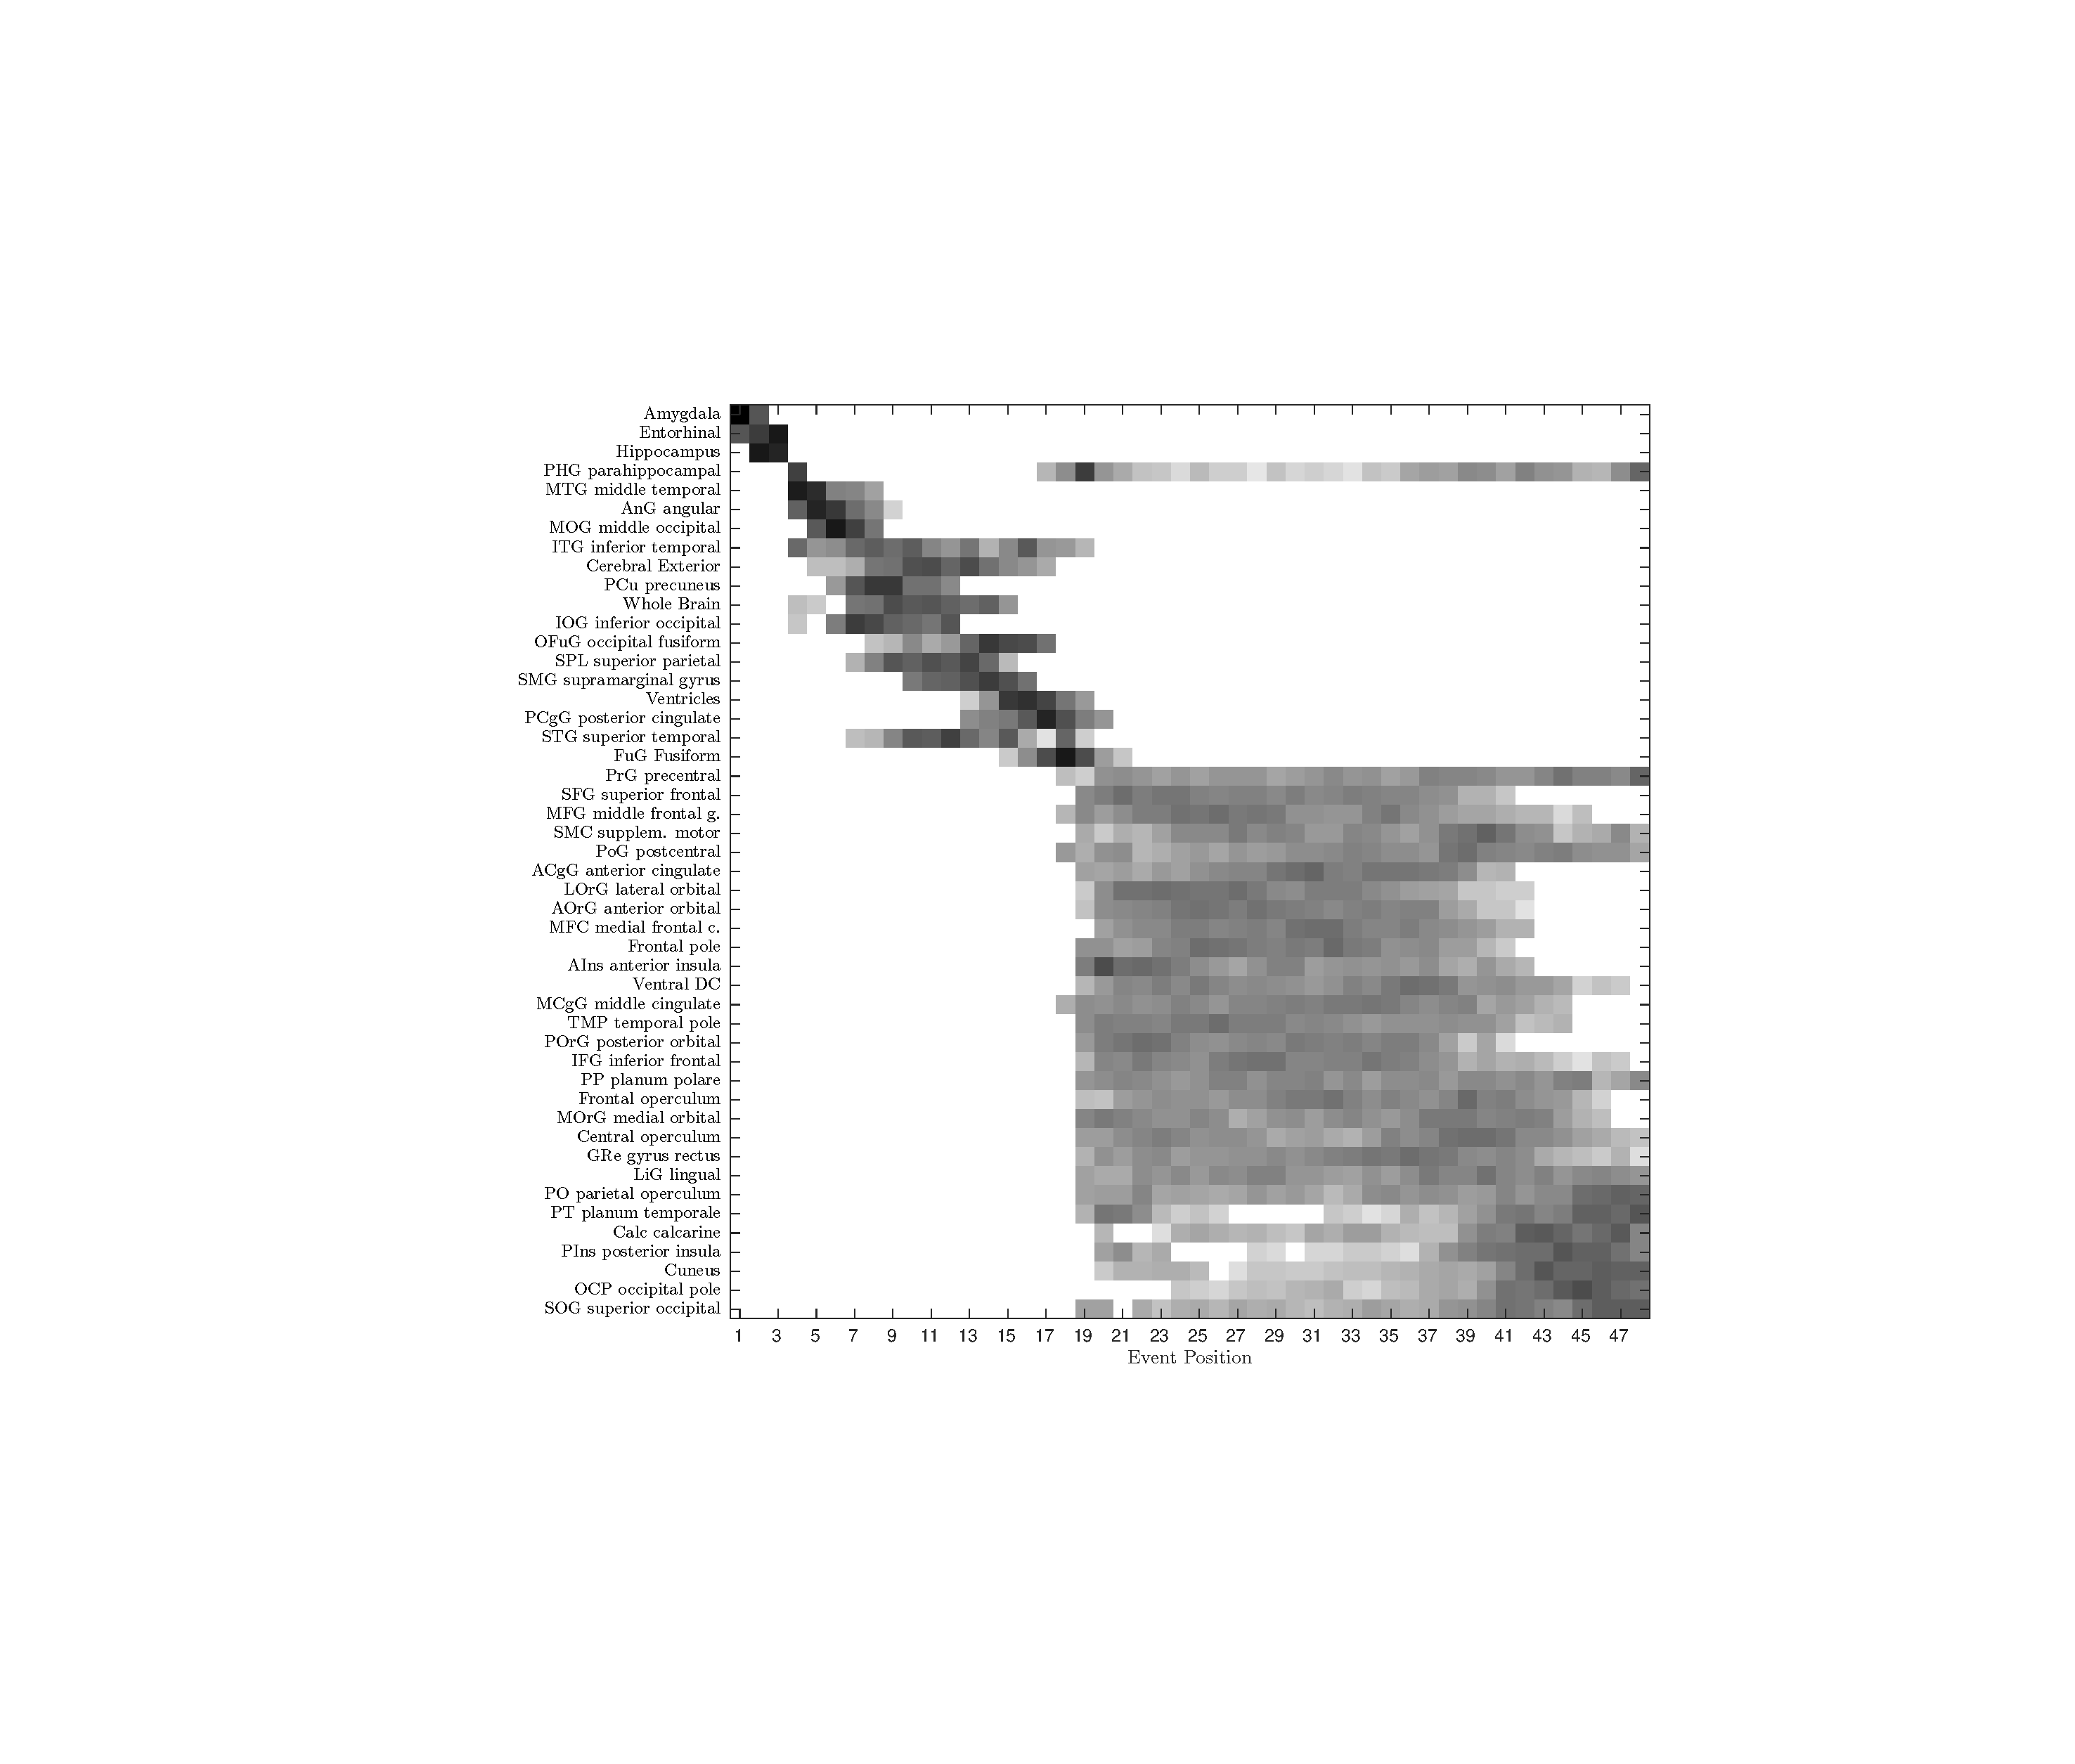
\includegraphics[scale=0.4]{../code/toyEBMs/figures/small5/posVarianceMatrix.pdf}};
  
  \draw (ordering.east) -| (1.5,0.3) -- (2.5,0.3);
  \draw (samples.east) -| (5.7,3);
  
  \draw (4,2.7) |- (7,3) -- (7,2.7);
  \draw (2.7,2) -| (2.5,-1.2) -- (2.7,-1.2);
  
\end{tikzpicture}
\caption[Event-based model - MCMC sampling diagram]{MCMC sampling and positional variance computation. MCMC sampling finds a series of $T$ samples, which are then used to derive the \emph{characteristic ordering}, where events are ordered according to their average position in the MCMC samples. Entries $M(i,j)$ in the positional variance matrix stores the relative number of times each event appeared in each position in the sequence. The events in the positional variance matrix are ordered according to the characteristic ordering.}
\end{figure}


\subsection{Event Sequence Estimation}
\label{sec:model_est}

Applying Bayes' theorem  we can get the posterior on the sequence:

\begin{equation}
 p(S|X) = \frac{p(S)p(X|S)}{p(X)}
\end{equation}

As the marginal distribution $p(X)$ is analytically intractable, one can use a Markov-chain Monte Carlo (MCMC) algorithm to sample from the posterior $p(S|X)$. A detailed description on how the MCMC algorithm works is given is section \ref{sec:MCMC}. One assumes flat priors on the sequence $S$ as any sequence could be equally likely.

In the MCMC phase, at each iteration the sequence $S$ can be perturbed by swapping two randomly chosen events. This perturbation rule has been used by Fonteijn et al. \cite{fonteijn2012event}. However, another perturbation method used by Young et al. \cite{young2014data} randomly selects a source and target event and places the source event after the target event, sliding the other biomarkers accordingly. See figure \ref{fig:backgr_mcmc_perturb} for a representation of the two perturbation rules. The resulting sequence $S^{new}$ is accepted with probability $p = min(1, a)$ where $ a = p(X|S^{new})/p(X|S)$. Otherwise the old sequence is stored and the process is repeated. As MCMC depends on accurate initialisation, one also runs a greedy ascent algorithm in order to find the sequence with the highest likelihood. The greedy ascent is very similar to the MCMC phase, the only difference being that $a$ is set to 1 if $p(X|S^{new}) > p(X|S)$ and to zero otherwise. Depending on the number of biomarkers, the greedy ascent is run for a few thousand iterations and repeated 10 times, with different random permutations of integers $1,\dots,N$ as the starting position. The maximum likelihood sequence obtained from greedy ascent is then used to initialise MCMC sampling, which usually runs for at least 100,000 iterations, again depending on problem size.

The resulting MCMC-sampled sequences are usually plotted in a positional variance matrix $M$, which is a compact way to represent uncertainty in the event ordering. Each element $M(i,j)$ represents the proportion of times event $E_{s(i)}$ appeared on position $j$ in the sampled sequences, given some \emph{master sequence} $S$. $S$ is usually set to be the maximum likelihood sequence or the \emph{characteristic ordering}, which is given by the average position of the events in the MCMC samples \cite{fonteijn2012event}. The characteristic sequence is particularly useful in plotting positional variance matrices from cross-validation or bootstrapping.

\begin{figure}
\centering
\begin{subfigure}[b]{0.45\textwidth}
 \centering
 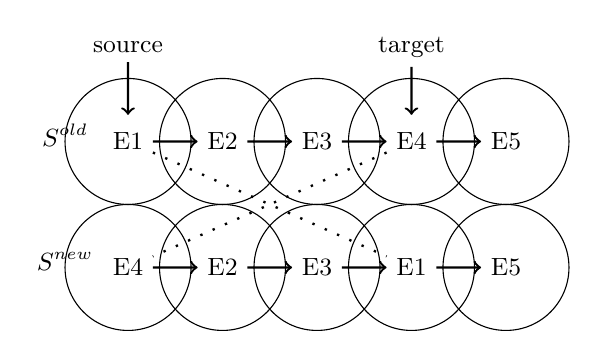
\begin{tikzpicture}[scale=0.8]
  \tikzstyle{every node}=[font=\small]


  \draw (-5,3) circle [radius=\nodeRad] node (E1) {E1};
  \draw (-3.5,3) circle [radius=\nodeRad] node (E2) {E2};  
  \draw (-2,3) circle [radius=\nodeRad] node (E3) {E3};
  \draw (-0.5,3) circle [radius=\nodeRad] node (E4) {E4};
  \draw (1,3) circle [radius=\nodeRad] node (E5) {E5};  
  \node (descold) at (-6,3.1) {$S^{old}$};
  \node (src) at (-5,4.5) {source};
  \node (trg) at (-0.5,4.5) {target};
  
  \draw[->,line width=0.3mm] (E1) -- (E2);
  \draw[->,line width=0.3mm] (E2) -- (E3);
  \draw[->,line width=0.3mm] (E3) -- (E4);
  \draw[->,line width=0.3mm] (E4) -- (E5);
  \draw[->,line width=0.3mm,shorten >=3pt] (src) -- (E1);
  \draw[->,line width=0.3mm,shorten >=3pt] (trg) -- (E4);  
  
  \draw (-5,1) circle [radius=\nodeRad] node (E4b) {E4};
  \draw (-3.5,1) circle [radius=\nodeRad] node (E2b) {E2};  
  \draw (-2,1) circle [radius=\nodeRad] node (E3b) {E3};
  \draw (-0.5,1) circle [radius=\nodeRad] node (E1b) {E1};
  \draw (1,1) circle [radius=\nodeRad] node (E5b) {E5};
  \node (descnew) at (-6,1.1) {$S^{new}$};
  
  \draw[->,line width=0.3mm] (E4b) -- (E2b);
  \draw[->,line width=0.3mm] (E2b) -- (E3b);
  \draw[->,line width=0.3mm] (E3b) -- (E1b);
  \draw[->,line width=0.3mm] (E1b) -- (E5b);
  
  \draw[loosely dotted, line width=0.3mm] (E1) -- (E1b);
  \draw[loosely dotted, line width=0.3mm] (E4) -- (E4b);  
 
  
\end{tikzpicture}
\caption{Fonteijn et al. \cite{fonteijn2012event}}
\end{subfigure}
%   ~
\begin{subfigure}[b]{0.45\textwidth}
 \centering
 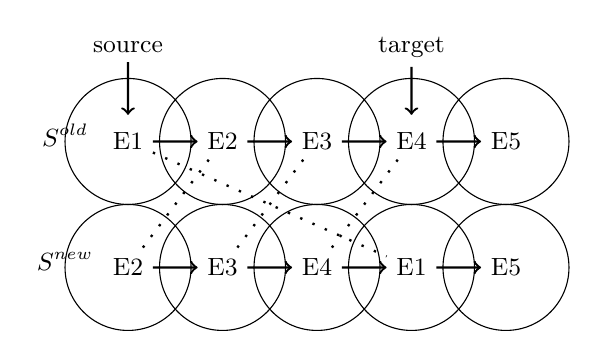
\begin{tikzpicture}[scale=0.8]
  \tikzstyle{every node}=[font=\small]


  \draw (-5,3) circle [radius=\nodeRad] node (E1) {E1};
  \draw (-3.5,3) circle [radius=\nodeRad] node (E2) {E2};  
  \draw (-2,3) circle [radius=\nodeRad] node (E3) {E3};
  \draw (-0.5,3) circle [radius=\nodeRad] node (E4) {E4};
  \draw (1,3) circle [radius=\nodeRad] node (E5) {E5};  
  \node (descold) at (-6,3.1) {$S^{old}$};
  \node (src) at (-5,4.5) {source};
  \node (trg) at (-0.5,4.5) {target};
  
  \draw[->,line width=0.3mm] (E1) -- (E2);
  \draw[->,line width=0.3mm] (E2) -- (E3);
  \draw[->,line width=0.3mm] (E3) -- (E4);
  \draw[->,line width=0.3mm] (E4) -- (E5);
  \draw[->,line width=0.3mm,shorten >=3pt] (src) -- (E1);
  \draw[->,line width=0.3mm,shorten >=3pt] (trg) -- (E4);  
  
  \draw (-5,1) circle [radius=\nodeRad] node (E2b) {E2};
  \draw (-3.5,1) circle [radius=\nodeRad] node (E3b) {E3};  
  \draw (-2,1) circle [radius=\nodeRad] node (E4b) {E4};
  \draw (-0.5,1) circle [radius=\nodeRad] node (E1b) {E1};
  \draw (1,1) circle [radius=\nodeRad] node (E5b) {E5};
  \node (descnew) at (-6,1.1) {$S^{new}$};
  
  \draw[->,line width=0.3mm] (E2b) -- (E3b);
  \draw[->,line width=0.3mm] (E3b) -- (E4b);
  \draw[->,line width=0.3mm] (E4b) -- (E1b);
  \draw[->,line width=0.3mm] (E1b) -- (E5b);
  
  \draw[loosely dotted, line width=0.3mm] (E1) -- (E1b);
  \draw[loosely dotted, line width=0.3mm] (E2) -- (E2b);
  \draw[loosely dotted, line width=0.3mm] (E3) -- (E3b);
  \draw[loosely dotted, line width=0.3mm] (E4) -- (E4b);  
 
  
\end{tikzpicture}
\caption{Young et al. \cite{young2014data}}
\end{subfigure}

\caption[MCMC perturbation rules]{MCMC perturbation rules used by (a) Fonteijn et al. \cite{fonteijn2012event} and (b) Young et al. \cite{young2014data}. Both methods assume randomly selected source and target events. The method by Fonteijn et al. only swaps the source event (E1) with the target event (E4). On the other hand, the perturbation used by Young et al. moves a source event after a target event and slides the other biomarkers accordingly.}
\label{fig:backgr_mcmc_perturb}
\end{figure}

\subsection{MCMC sampling - Metropolis Hastings}
\label{sec:MCMC}

%TODO: picture with proposal and sampling distribution

In order to sample the event ordering, one can use the Metropolis Hastings algorithm, which is a Markov chain Monte Carlo sampling  method. The original Metropolis algorithm was proposed by Metropolis et al. in 1953 \cite{metropolis1953equation}. W. K. Hastings extended it to a more general case in 1970 \cite{hastings1970monte}. 

Suppose we have a function $f(x)$ which is proportional to a probability distribution $p(x)$, which we need to take samples from. It is often the case in practice that the normalisation factor is not known because it is extremely difficult to compute it. The Metropolis Hastings algorithm works by producing a sequence of samples $X_0,X_1,\dots,X_n$ where each sample $X_{t+1}$ is generated from $X_t$ using a proposal distribution $Q(X_{t+1}|X_t)$. At each iteration, a candidate sample $X_{cand}$ is generated from the proposal distribution $Q(X_{t+1}|X_t)$. A probability ratio $a$ is calculated as follows:

\begin{equation}
 a = \frac{f(X_{cand})}{f(X_{t})} \frac{Q(X_t|X_{cand})}{Q(X_{cand}|X_t)}
\end{equation}
Finally, the sample $X_{cand}$ is accepted with probability $\min(1, a)$. Note that in most cases the \emph{proposal distribution} is symmetric, i.e. $Q(X_t|X_{cand}) = Q(X_{cand}|X_t)$, in which case the ratio $a$ becomes:

$$a = \frac{f(X_{cand})}{f(X_{t})}$$

\begin{myalgo}[Metropolis-Hastings algorithm]
 \begin{enumerate}[label*=\arabic*.]
  \item Choose a starting point $X_1$
  \item for $t=2$ to $T$
  \begin{enumerate}[label*=\arabic*.]
    \item Draw a candidate sample $X^{cand}$ from the proposal distribution $Q(X|X^t)$
    \item Compute the acceptance ratio $a$ as follows:
       $$a = \frac{f(X_{cand})}{f(X_{t})} \frac{Q(X_t|X_{cand})}{Q(X_{cand}|X_t)}$$
    \item Draw a random number $r$ from the unit interval $[0,1]$
    \item Accept the candidate sample $X^{cand}$ only if $a \ge r$. That is:
       $$ X^{t+1} = \begin{cases} \hfill X^{cand} &\mbox{if } a \ge r \\ 
					      X^t & \mbox{ otherwise }\end{cases}$$
    
  \end{enumerate}
  
 \end{enumerate}

\end{myalgo}


\subsection{Mixture Models For Data Likelihood}
\label{sec:mix_models}

In equation \ref{eq:ebm1} we need to model the distributions $p\left(x_{i,j} | E_{i} \right)$ and $p\left(x_{i,j} | \neg E_{i}\right)$ using the measurements in $X$. However, the fact that a subject is a control or patient does not give any information whether event $E_{i}$ has occurred. Therefore, it is necessary to use a mixture model, whose components will correspond to $p\left(x_{i,j} | E_{i} \right)$ and $p\left(x_{i,j} | \neg E_{i}\right)$ respectively. The particular choice of the model depends on the data that is being modelled. Fonteijn et al. \cite{fonteijn2012event} used a Gaussian distribution for $p\left(x_{i,j} | \neg E_{i}\right)$ and a uniform distribution for $p\left(x_{i,j} | E_{i} \right)$. On the other hand, Young et al. \cite{young2014data} used two Gaussian distributions for both distributions and applied some constraints on their mean and variance. The models are fit using numerical optimisation or Expectation-Maximisation (EM).

\subsection{Patient Staging and Diagnosis Prediction}
\label{sec:staging}

After the maximum likelihood sequence has been found using the greedy ascent method described in section \ref{sec:model_est}, each subject can be assigned a stage $k$ as follows:

\begin{equation}
\label{eq:staging}
 k = \argmax_k p(k) p(X_j | S, k) = p(k) \prod_{i=1}^k p\left(x_{s(i),j} | E_{s(i)} \right) \prod_{i=k+1}^N p\left(x_{s(i),j} | \neg E_{s(i)}\right) 
\end{equation}
 

As before, the prior $p(k)$ is assumed to be uniform. It should be noted that stages range from zero to $N$, the number of events. If a subject is at stage $k$ it means that all events up to and including $k$ have occurred while the events after $k$ have not occurred. 

One can use patient stages to classify subjects into controls and AD, or any other available subgroups, using a simple method by Young et al. \cite{young2014data}. Given a threshold stage $t$, one can predict all subjects having a stage less than or equal to $t$ to be controls and all subjects with stages greater than $t$ to be patients. The optimal threshold is the one which maximises the balanced accuracy, defined as follows:

\begin{equation}
 Accuracy = \frac{TP + TN}{TP + FP + FN + TN}
\end{equation}
where $TP$, $FP$, $FN$, $TN$ represent the number of true positive, false positive, false negative and true negative subjects respectively. After the optimal threshold is found, one can also compute the sensitivity and specificity defined as follows:

\begin{equation}
 Sensitivity = \frac{TP}{TP + FN}
\end{equation}

\begin{equation}
 Specificity = \frac{TN}{TN + FP}
\end{equation}



\subsection{Advantages and Limitations}

% Advantages
The event-based model by Fonteijn et al. \cite{fonteijn2012event} has several advantages. It is a data-driven progression model which does not use a-priori defined clinical stages, which can often be biased and limit the temporal resolution of the model. Moreover, it does not require longitudinal data, which makes it very useful for analysing rare types of dementia for which comprehensive longitudinal datasets do not exist. The Bayesian framework in which it is formulated also allows it to estimate uncertainty in the abnormality sequence. The model can also easily combine data from different modalities.  

% Limitations
The current model has several limitations. The trajectory parameters are modelled as step functions, which is a strong assumption given the continuous nature of almost every MRI and CSF biomarker commonly used in the field. Secondly, in the fitting process the parameters and sequence are assumed independent and therefore fitted separately. Third, the model assumes all biomarker measurements are independent with each other and also across different visits of the same subject.  Finally, the model also assumes that all subjects follow the same progression sequence, which is not the case in heterogeneous datasets such as ADNI.


\section{Differential Equation Model}
\label{sec:dem}

The differential equation model (DEM) \cite{ashford2001modeling,yang2011quantifying,sabuncu2011dynamics,villemagne2013amyloid} constructs the biomarker trajectories from the change in biomarker values between different visits. In many datasets such as ADNI, the biomarker scores $s$ are observed for each subject over a few visits. By determining how these scores change ($\Delta s$) over time ($t$) during a specified time interval $\Delta t$, the temporal rate of progression ($\Delta s/\Delta t$) can be modelled as a function of the mean biomarker value $f(s)$ \cite{ashford2001modeling}:

\begin{equation}
\label{eq:dem_1}
 \frac{\Delta s}{\Delta t} \approx f(s)
\end{equation}

The model given by $f(s)$ can be for example linear, polynomial or non-parametric models such as Gaussian Processes (GP). We then perform a line integral along $f(s)$ to recover $s(t)$. More explicitly, if we take the limit as $\Delta \xrightarrow{} 0$ from Eq. \ref{eq:dem_1}, we get that:

\begin{equation}
\label{eq:dem2}
lim_{\Delta t \xrightarrow{}  0} \frac{\Delta s}{\Delta t} = \frac{\delta s}{\delta t} = f(s)
\end{equation}

Solving this numerically is done using the Euler method. We set an initial $(t_0,s_0)$ and small increment step $\delta t$ and finding the next pair $(t_1, s_1)$ as follows:

\newcommand\numberthis{\addtocounter{equation}{1}\tag{\theequation}}

\begin{align*}
 t_1 &= t_0 + \delta t \\
 s_1 &= s_0 + f(s_0) \delta t \numberthis \label{eq:dem3}
\end{align*}

This is the repeated until the full curve defined by $(t_0, s_0), (t_0, s_0), \dots, (t_n, s_n)$ is reconstructed. The process is repeated independently for the other biomarkers. 

\subsection{Advantages and Limitations}

The differential equation model has several advantages. It is a fully data-driven method that does not require a-priori defined clinical categories. In contrast to the event-based model, it can estimate non-parametric biomarker trajectories which makes minimal assumptions on the shape of the biomarker trajectories, with the only real constraint being monotonicity. 

The model has several limitations. First of all, the biomarker trajectories are fit independently, which requires alignment on the temporal axis after they are recovered. Secondly, in this formulation the model does not allow to directly estimate uncertainty in the trajectory values along the y-axis. The only option for estimating uncertainty is by integrating posterior samples of the differential model and then aligning them all on the temporal axis. A third limitation is that the model is very sensitive to noise in the biomarker measurements. 


\section{The Disease Progression Score model}
\label{sec:dps}

The disease progression score (DPS) model was proposed by Jedynak et al. \cite{jedynak2012computational}. It is based on three main assumptions:
\begin{itemize}
 \item Subjects follow a common disease progression but they have a different age on onset and progression speed.
 \item Each biomarker trajectory is a monotonic curve that follows a sigmoidal shape
 \item The speed of progression of each subject is the same across the entire disease time-course.
\end{itemize}

The model estimates the optimal shape of the biomarker trajectories while estimating a disease progression score for each subject, which is the stage along the disease time course. The disease progression score $s_{ij}$ for subject $i$ at visit $j$ is defined as a linear transformation of age $t_{ij}$:

\begin{equation}
\label{eq:dps}
 s_{ij} = \alpha_i t_{ij} + \beta_i
\end{equation}
% sigmoidal functions
where $\alpha_i$ and $\beta_i$ represent the speed of progression and time shift (i.e. disease onset) of subject $i$. 

The DPS model assumes that biomarker measurements are independent and follow a sigmoidal trajectory $f(s)$ given the disease progression score $s$. The sigmoidal function for biomarker $k$ is parametrised as $\theta_k = [a_k,b_k,c_k,d_k]$ where:

\begin{equation}
 f(s;\theta_k) = \frac{a_k}{1+exp(-b_k(s-c_k))} + d_k
\end{equation}
where $d_k$ is the minimum value, $d_k+a_k$ is the maximum value, $a_kb_k/4$ is the maximum slope and $c_k$ is the inflexion point. Previous work has shown that sigmoidal curves provide a better fit for biomarker data compared to linear models \cite{sabuncu2011dynamics,caroli2010dynamics}. The value $y_{ijk}$ of biomarker $k$ from subject $i$ at visit $j$ is a normally distributed random variable:
\begin{equation}
 p(y_{ijk} | \alpha_i, \beta_i, \theta_k, \sigma_k) = N(y_{ijk} | f(\alpha_i t_{ij} + \beta_i; \theta_k), \sigma_k )
\end{equation}
We further define $I$ to be the set of all triplets $(i,j,k)$ for which measurements are available. Assuming independence across all measurements we get the following model likelihood:
\begin{equation}
 p(y | \alpha, \beta, \theta, \sigma) = \prod_{(i,j,k) \in I} p(y_{ijk} | \alpha_i, \beta_i, \theta_k, \sigma_k)
\end{equation}
where $y = [y_{ijk}]$ for $(i,j,k) \in I$. Vectors $\alpha = [\alpha_1, \dots, \alpha_S]$ and $\beta = [\beta_1, \dots, \beta_S]$, where $S$ is the number of subjects, denote the stacked parameters for the subject shifts. Vectors $\theta = [\theta_1, \dots, \theta_K]$ and $\sigma = [\sigma_1, \dots, \sigma_K]$, with $K$ being the number of biomarkers, represent the stacked parameters for the sigmoidal trajectories and measurement noise specific to each biomarker.

The parameters of the model are therefore $\Theta = [\alpha, \beta, \theta, \sigma]$ and the log-likelihood function associated with it is:
\begin{equation}
 l(\alpha, \beta, \theta, \sigma) = \sum_{(i,j,k) \in I} log \sigma_k + \frac{1}{2 \sigma_k ^2} \left( y_{ijk} - f(\alpha_i t_{ij})\right)
\end{equation}

\subsection{Model fitting}

Model fitting is done by alternating between optimising the sigmoidal parameters $\sigma$ and the subject specific parameters $\alpha, \beta$ using the method of least squares. Figure \ref{fig:algo_dps} show the fitting procedure. In line \ref{alg:init}, we initialise $\alpha_i = 1$, $\beta_i = 0$ for every $i$. On lines \ref{alg:theta} and \ref{alg:sigma} the optimal parameters for every biomarker trajectory are computed. On line \ref{alg:alpha} the subject specific shifts and progression speeds are found. Sometimes unfeasible parameters can be retrieved, so on line \ref{alg:identif} the parameters are mapped into the feasible space. In order to make the model identifiable, parameters $\alpha_i$ and $\beta_i$ are rescaled for every subject on line \ref{alg:rescale} so that the disease progression scores of healthy controls have a mean $\mu_N$ of 0 and a standard deviation $\sigma_N$ of 1.

\begin{algorithm}
%  \KwData{this text}
%  \KwResult{how to write algorithm with \LaTeX2e }
 Initialise $\alpha^{(0)}$, $\beta^{(0)}$\;\label{alg:init}
 \For{$l=1$ to $L$}{
    \For{$k=1$ to $K$}{
      $\theta_k^{(1)} = \argmin_{\theta_k} \sum_{(i,j) \in I_k} (y_{ijk} - f(\alpha_i^{(0)} t_{ij} + \beta_i^{(0)} | \theta_k))^2$\label{alg:theta}\\
      $\sigma_k^{(1)^2} = \frac{1}{|I_k-2I-4|} \sum_{(i,j) \in I_k} (y_{ijk} - f(\alpha_i^{(0)} t_{ij} + \beta_i^{(0)} | \theta_k))^2$\label{alg:sigma}
    }
    \For{$i=1$ to $I$}{
      $\alpha_i^{(1)}, \beta_i^{(1)} = \argmin_{\alpha_i, \beta_i}  \sum_{(j,k) \in I_i} \frac{1}{\sigma_k^{(1)^2}}(y_{ijk} - f(\alpha_i t_{ij} + \beta_i | \theta_k^{(1)}))^2$\label{alg:alpha}
    }
    $\alpha^{(0)}=\alpha^{(1)}, \beta^{(0)}=\beta^{(1)}$\label{alg:update}
 }

  \For{$k=1$ to $K$}{
    \If{$b_k < 0$}{
      $a_k^{(1)} = -a_k^{(1)}, b_k^{(1)} = -b_k^{(1)}, d_k^{(1)} = d_k^{(1)}+a_k^{(1)}$\label{alg:identif}\\
    }
  }
  
  \For{$i=1$ to $I$}{
    $\alpha_i = \frac{\alpha_i}{\sigma_N}, \beta_i = \frac{\beta_i - \mu_N}{\sigma_N}$\label{alg:rescale}
  }
 \caption{The optimisation procedure for the disease progression score by \cite{jedynak2012computational}.}
 \label{fig:algo_dps}
\end{algorithm}


\subsection{Advantages and Limitations}

The model by Jedynak et al. \cite{jedynak2012computational} has several advantages. As opposed to the differential equation model, the model automatically aligns the biomarker trajectories on the temporal axis. Furthermore, compared to the event-based model by \cite{fonteijn2012event}, the biomarker trajectories are modelled as sigmoidal trajectories instead of step functions and each subject has an associated time shift and progression speed. 

The model has several limitations. The main limitation of this model is that the trajectories are assumed to be sigmoidal, which is not necessarily the case for many biomarkers in ADNI (e.g. MRI volumes or cortical thickness) that don't show any signs of plateauing. Furthermore, each subject is assumed to follow the same progression pattern, which is not true in many heterogeneous datasets such as ADNI.

\section{The Self-Modelling Regression model}
\label{sec:semor}

Self-modelling regression (SEMOR) is a method that fits several curves under the assumption of a common shape \cite{donohue2014estimating}. This approach has been used by Donohue et al. \cite{donohue2014estimating} to estimate non-parametric biomarker trajectories with linear subject-specific effects. We assume that $Y_{ij}$ is the measurement of biomarker $j$ in subject $i$, $g_j$ is a continuously differentiable monotone function, $\gamma_i \sim N(0, \sigma_{\gamma}^2)$ is the time shift for subject $i$. The model is defined as follows:
\begin{equation}
 \label{eq:semor1}
 Y_{ij}(t) = g_j(t +\gamma_i)+\alpha_{0ij} + \alpha_{1ij}t+\epsilon_{ij}(t)
\end{equation}
where $\alpha_{0ij}, \alpha_{1ij} \sim N(0, \Sigma_j)$ model a linear perturbation of the non-parametric trajectory $g_j$ for subject $i$ and biomarker $j$, $t$ is the time and $\epsilon_{ij}(t) \sim N(0, \sigma_j)$ is the measurement noise.  

\subsection{Parameter fitting}

Fitting the model is done by iteratively estimating each set of parameters $(g_j, \gamma_i, \alpha)$ until convergence of the Residual Sum of Squares (RSS). The algorithm makes use of the following residuals:
\begin{equation}
\begin{cases}
  R_{ij}^g(t) = Y_{ij}(t) - \alpha_{0ij} - \alpha_{1ij}t & \qquad E\left[ R_{ij}^g(t) | g_j, t, \gamma_i \right] = g_j(t+\gamma_i)\\
  R_{ij}^{\alpha}(t) = Y_{ij}(t) - g_j(t+\gamma_i) & \qquad E\left[ R_{ij}^{\alpha}(t) | \alpha_{0ij}, \alpha_{1ij}, t \right] = \alpha_{0ij} + \alpha_{1ij}t\\
  R_{ij}^{\gamma}(t) = t-g_j^{-1}(Y_{ij}(t)) & \qquad E\left[ R_{ij}^{\gamma}(t) | \gamma_i \right] \approx g_j^{-1}(g_j(t+\gamma_i))-t = \gamma_i\\  
\end{cases}  
\end{equation}

Using the above residuals, the model is fit by initialising $\gamma_i$ and iterating the following steps\cite{donohue2014estimating}:
\begin{enumerate}
 \item Given $\gamma_i$, estimate $g_j$ by setting $\alpha_{0ij} = \alpha_{1ij} = 0$ and iterating the following subroutine:
 \begin{enumerate}
  \item Estimate $g_j$ by a monotone curve fit on $R_{ij}^g(t)$
  \item Estimate $\alpha_{0ij}, \alpha_{1ij}$ using the linear mixed model of $R_{ij}^{\alpha}(t)$. Repeat steps a and b until convergence of each $RSS_j = \sum_{it} \left[ Y_{ij}(t)-g_j(t+\gamma_i)-\alpha_{0ij}-\alpha_{1ij}t \right]^2 $
 \end{enumerate}
 
 \item Given the estimated $g_j$, set $\alpha_{0ij} = \alpha_{1ij} = \epsilon_{ij}(t) = 0$ and estimate each $\gamma_i$ with the average of $R_{ij}$ over all $j$ and $t$. Steps 1 and 2 are repeated until convergence of the total $RSS = \sum_{ijt} \left[ Y_{ij}(t)-g_j(t+\gamma_i)-\alpha_{0ij}-\alpha_{1ij}t \right]^2 $

\end{enumerate}

\subsection{Advantages and limitations}

The model have many advantages. It robustly models the average trajectory using a non-parametric model, in contrast with previous approaches \cite{jedynak2012computational}. Moreover, it also models unique trajectories for each subject as linear deviations from the average trajectories using a mixed effects model. Each subject also has it's own temporal shift. 

One limitation of the model is that it does not model different progression speeds for each individual. Also, estimating all the subject-specific parameters $(\alpha_{0ij}, \alpha_{1ij}, \gamma_i)$ requires suitable priors and many longitudinal measurements, which might not be available in some datasets. Moreover, it also assumes that biomarker measurements are independent, which makes it unsuitable for modelling large sets of correlated biomarkers such as vertex-wise cortical thickness measures or voxel-wise amyloid burden. 

\section{The Manifold-based mixed effects model}
\label{sec:manifold}

The manifold-based mixed effects model was introduced by Schiratti et al. in 2015 \cite{schiratti2015mixed}. The model generalises a previous linear mixed effects model by \cite{datar2012mixed} to account for time shifts and describes it in a Riemannian manifold setting. Let us assume we observe $p$ individuals, each having $n_i$ observations obtained at times $t_{i,1} < \dots < t_{i,n_i}$, each having $y_i,1, \dots, y_{i,n_i}$ biomarker measurements. For a point $p_0 \in M$, $v_0 \in T_{p_0}M$ we define $\gamma_{p_0,t_0,v_0} = Exp_{t_0,p_0}(\alpha_iv_0)(.)$ as the geodesic which passes through point $p_0$ at time $t_0$ with velocity $v_0$. We also consider $t_{i,j}$ and $y_{i,j}$ as the age and measurement for one biomarker in subject $i$ at visit $j$. This gives us the following model:

\begin{equation}
\label{eq:manifold1}
 y_{i,j} = Exp_{t_0+\tau_i,p_0}(\alpha_iv_0)(t_i,j) + \epsilon_{i,j}
\end{equation}
where
\begin{equation}
\label{eq:manifold2}
\begin{cases}
  \alpha_i = exp(\nu_i)\\
  \nu_i \sim \bigotimes_{i=1}^p N(0, \sigma_{\nu}^2)\\  
  \tau_i \sim \bigotimes_{i=1}^p N(0, \sigma_{\tau}^2)\\  
  \epsilon_{i,j} \sim \bigotimes_{i,j} N(0, \sigma^2)\\  
\end{cases}
\end{equation}
The model assumes that each $\eta_i$ and $\tau_i$ are independent. The parameters of the model are $\theta = [p_0, t_0, v_0, \sigma_{\eta}, \sigma_{\tau}, \sigma]$. The model above can be re-written as:
\begin{align*}
  y_{i,j} &= \gamma_{p_0,t_0,v_0}(\alpha_iv_0(t_{i,j}-t_0-\tau_i))+\epsilon_{i,j}\\
          &= \gamma_i(t_{i,j})+\epsilon_{i,j} \numberthis \label{eq:manifold3}
\end{align*}
where $\gamma_i$ is the subject specific trajectory that is modelled as an affine reparametrisation of the average trajectory $\gamma_{p_0,t_0,v_0}$. The model described here is univariate. However, an extension of he model has been published by Schiratti et al. \cite{schiratti2015learning} which extends this framework to a multivariate analysis. 

\subsection{The straight lines model}

If we assign the canonical (i.e. Euclidean) metric to the manifold $M=\mathbb{R}$, we get the "straight lines" model:
\begin{equation}
 y_{i,j} = p_0 + \alpha_i v_0(t_{i,j}-t_0-\tau_i)+\epsilon_{i,j}
\end{equation}

\subsection{The logistic curve model}

Some biomarkers such as Mini-Mental State Examination or other cognitive tests are bounded in a specific interval that can be mapped to (0,1). In order to give the (0,1) interval a Riemannian manifold structure we need to equip it with a Riemannian metric. For all points $p_0 \in M$ we define $g_0$ to be the inner product $g_{p_0}(u,v) = uM(p_0)v$ where $M(p_0) = \frac{1}{p_0^2(1-p_0)^2)}$. This results in the geodesics of $M$ to be logistic curves of the form $t \rightarrow (1+a\ \text{exp}(-rt))^{-1} $ \cite{schiratti2015mixed}. Therefore, the model from Eq. \ref{eq:manifold1} writes:
\begin{equation}
 y_{i,j} = \left[ 1+\left(\frac{1}{p_0}-1\right)\text{exp}\left( -\frac{\alpha_iv_0}{p_0(1-p_0)}(t_{i,j}-t_0-\tau_i)\right) \right]^{-1}+\epsilon_{i,j}
\end{equation}

\subsection{Advantages and limitations}

The model has several strengths and weaknesses. The main strength lies in the flexible Riemannian manifold framework, that allows one to create different models depending on how the inner product is defined. Moreover, the model estimates subject specific trajectories $\gamma_i$, time shifts $\tau_i$ and progression speeds $\alpha_i$. However, one of the limitations of the model is that it assumes a parametric form of the biomarker trajectories (i.e. sigmoidal). 

\section{The voxelwise disease progression model}
\label{sec:bilgel_voxelwise}

A voxelwise disease progression model has been introduced in 2016 by Bilgel et al. \cite{bilgel2016multivariate}. This model allows the discovery of patterns of atrophy that are not confined to a given region of interest (ROI). Since the input data is represented by voxel-wise measurements such as amyloid burden, a spatial correlation function is used to model correlation between voxel values. The model is built on the framework of the disease progression score by Jedynak et al. \cite{jedynak2012computational}. 

Let us assume that $t_{ij}$ represent the age for subject $i$ at visit $j$. The progression score $s_{ij}$ for subject $i$ at visit $j$ is an affine transformation of age $t_{ij}$:

\begin{equation}
 \begin{cases}
 s_{ij} = \alpha_i t_{ij} + \beta_i = \textbf{q}_{ij}^T\textbf{u}_i\\
 \textbf{u}_i \sim N_2(\textbf{m}, V(\boldsymbol{\nu}))
\end{cases}
\end{equation}
where $\alpha_i$, $\beta_i$ are the progression speed and time shift of subject $i$, $\textbf{q}_{ij} = [t_{ij}, 1]^T$ and $\textbf{u}_{i} = [\alpha_i, \beta_i]^T$. The prior covariance matrix $V$ is modelled as a 2 $\times$ 2 positive definite matrix that has a Log-Cholesky parametrisation given by $\boldsymbol{\nu}$. More precisely, if we consider a matrix $U$ such that $V = UU^T$ and $U = \begin{bmatrix}
    U_{11} & U_{12} \\
    0 & U_{22}\\
\end{bmatrix}$, then $\boldsymbol{\nu} = [logU_{11}, logU_{12}, logU_{22}]$

Furthermore, let us denote by $\textbf{y}_{ij}$ the $K \times 1$ vector of biomarker measurements for subject $i$ at visit $j$. The longitudinal trajectories corresponding to these measurements are modelled as follows:

\begin{equation}
 \begin{cases}
  \textbf{y}_{ij} = \textbf{a}s_{ij}+\textbf{b}+\epsilon_{ij}\\
  \epsilon_{ij} \sim N_K(0,R(\boldsymbol{\lambda},\boldsymbol{\rho}))
 \end{cases}
\end{equation}
where $\textbf{a} = [a_1, \dots, a_K]^T$, $\textbf{b} = [b_1, \dots, b_K]^T$ are the coefficients of the linear model and $\epsilon_{ij}$ is the measurement noise that is independent and identically distributed across different subjects and visits. The matrix $R(\boldsymbol{\lambda},\boldsymbol{\rho})$ is the spatial covariance that is assumed to have the form $R = \Lambda C \Lambda$, where $\Lambda$ is a diagonal matrix with diagonal elements $\boldsymbol{\lambda}$ and $C$ is a correlation matrix that is parametrised by $\boldsymbol{\rho}$ \cite{bilgel2016multivariate}. This ensures that the matrix $R(\boldsymbol{\lambda},\boldsymbol{\rho})$ is positive definite. In order to model correlation among voxel measurements, the elements $C_{kk'}$ of matrix $C$ must be a function of the distance $d \equiv d(k,k')$ between voxels $k$ and $k'$. Several such options exist:
\begin{itemize}
 \item Exponential: $C_{kk'} = \text{exp}(-d/\rho)$
 \item Gaussian: $C_{kk'} = \text{exp}(-(d/\rho)^2)$
 \item Exponential: $C_{kk'} = \left(1+(d/\rho)^2\right)^{-1}$
 \item Spherical: $C_{kk'} = \left( 1 - \frac{3}{2}\frac{d}{\rho} + \frac{1}{2}\left(\frac{d}{\rho}\right)^{3} \right)$ if $d<\rho$
\end{itemize}
The model parameters are therefore $\boldsymbol{\theta} = [\textbf{m},\boldsymbol{\nu},\textbf{a},\textbf{b},\boldsymbol{\lambda},\boldsymbol{\rho}]$. The model is a mixed effects model where $\textbf{a}$, $\textbf{b}$ are the fixed effects and $\textbf{u}_i$ are the random effects. 

\subsection{Model fitting}

The model is fit using the Expectation-Maximisation (EM), described below. The complete data log-likelihood is:
\begin{align*}
 & l(\textbf{y}, \textbf{u}; \boldsymbol{\theta}) = \sum_i l(\textbf{y}_i, \textbf{u}_i; \boldsymbol{\theta}) =\\
 & -\frac{1}{2}\sum_{i,j}log|2\pi R|-\frac{1}{2}\sum_{i,j}\left(\textbf{y}_{ij}-Z_{ij}\textbf{u}_i-\textbf{b}\right)^T \\
 & -\frac{1}{2}\sum_{i} log|2\pi V|-\frac{1}{2}\sum_{i}(\textbf{u}_i-\textbf{m})^T V^{-1}(\textbf{u}_i-\textbf{m})
 \numberthis \label{eq:bilgel3}
\end{align*}

\subsubsection{E-step}

Let $(\textbf{y}, \textbf{u})$ be the complete data and $\boldsymbol{\theta}' = [\textbf{m}',\boldsymbol{\nu}',\textbf{a}',\textbf{b}',\boldsymbol{\lambda}',\boldsymbol{\rho}']$ be the parameters estimated at the previous EM iteration. Bilgel et al. \cite{bilgel2016multivariate} show that the E-step integral $Q(\boldsymbol{\theta}, \boldsymbol{\theta}')$ is proportional to $\sum_i \int \Phi(\tilde{\textbf{u}_i};\hat{\textbf{u}}'_i, \Sigma_i') l(\textbf{y}_i, \tilde{\textbf{u}}_i; \boldsymbol{\theta})d\tilde{\textbf{u}}_i$, where $\Phi$ is a multivariate normal probability density function with mean:

\begin{equation}
 \hat{\textbf{u}}'_i = \left( \sum_{j} Z'^T_{ij} R'^{-1} Z'_{ij} + V'^{-1}\right)^{-1}\left( \sum_{j} Z'^T_{ij} R'^{-1} (\textbf{y}_{ij}-\textbf{b}') + V'^{-1}\textbf{m}' \right)
\end{equation}
and covariance matrix $\Sigma'_{i}=\left( \sum_{j} Z'^T_{ij} R'^{-1} Z'_{ij} + V'^{-1}\right)^{-1}$. Evaluating the integral gives the following final form:

\begin{align*}
 & Q(\boldsymbol{\theta}, \boldsymbol{\theta}') = -\frac{1}{2} \sum_{ij}log|R| - \frac{1}{2}\sum_{ij}\left( \textbf{y}_{ij} - Z_{ij}\hat{\textbf{u}}'_i -\textbf{b}\right) - \frac{1}{2}\sum_{ij}Tr\left( Z^T_{ij} R^{-1} Z_{ij}\Sigma_i' \right) - \\
 & \frac{1}{2}\sum_{i}log|V| - \frac{1}{2}\sum_{i}\left( \hat{\textbf{u}}'_i - \textbf{m} \right)^T V^{-1} \left( \hat{\textbf{u}}'_i - \textbf{m} \right) - \frac{1}{2}\sum_i Tr\left( V^{-1} \Sigma_i'\right) \numberthis \label{eq:bilgel_e-step}
\end{align*}


\subsubsection{M-step}

At the M-step we need to find $\boldsymbol{\theta} = \argmax_{\boldsymbol{\theta}}Q(\boldsymbol{\theta}, \boldsymbol{\theta}')$. The full derivations are given in \cite{bilgel2016multivariate}, yielding the following updates:

\begin{equation}
\label{eq:bilgel_mstep1}
 \textbf{a} = \frac{\left( \sum_i \nu_i \right) \left( \sum_{ij} \textbf{y}_{ij}s'_{ij} \right) - \left( \sum_{ij} \textbf{y}_{ij} \right) \left( \sum_{ij}s'_{ij} \right)}{\left( \sum_i \nu_i \right) \left( \sum_{ij} \textbf{q}_{ij}^T \Sigma_i' \textbf{q}_{ij} + s_{ij}'^2 \right) - \left( \sum_{ij}s'_{ij} \right)^2}
\end{equation}

\begin{equation}
\label{eq:bilgel_mstep2}
 \textbf{b} = \frac{\left( \sum_{ij} \textbf{y}_{ij} \right) \left( \sum_{ij} \textbf{q}_{ij}^T \Sigma_i' \textbf{q}_{ij} + s_{ij}'^2 \right) - \left( \sum_{ij} \textbf{y}_{ij}s'_{ij} \right) \left( \sum_{ij} s'_{ij} \right)}{\left( \sum_i \nu_i \right) \left( \sum_{ij} \textbf{q}_{ij}^T \Sigma_i' \textbf{q}_{ij} + s_{ij}'^2 \right) - \left( \sum_{ij}s'_{ij} \right)^2}
\end{equation}

\begin{equation}
 \textbf{m} = \frac{1}{n}\sum_i \hat{\textbf{u}}'_i
\end{equation}

\begin{equation}
 \boldsymbol{\nu} = \argmax_{\boldsymbol{\nu}} Q(\boldsymbol{\theta}, \boldsymbol{\theta}')
\end{equation}

\begin{equation}
 \boldsymbol{\lambda}, \boldsymbol{\rho} = \argmax_{\boldsymbol{\lambda}, \boldsymbol{\rho}} Q(\boldsymbol{\theta}, \boldsymbol{\theta}')
\end{equation}

\subsection{Advantages and limitations}

The model by Bilgel et al. \cite{bilgel2016multivariate} has several advantages. First of all, it is specifically tailored for dealing with voxelwise measurements such as amyloid load by modelling the spatial correlations. Secondly, like the disease progression score by Jedynak et al. \cite{jedynak2012computational}, it estimates subject specific temporal shifts and progression speeds. 

The model has several limitations. First of all, the biomarker trajectories are assumed to be linear, which is a strong assumption especially for early many biomarkers such as amyloid, which start to plateau when subjects are in the MCI stages. Moreover, while it is necessary to incorporate a spatial correlation function due to the nature of the data, this has the effect of "blurring out" the image and is not suitable for some voxels that are close-by and undergo different trajectories. 

\section{The Network Diffusion Model}
\label{sec:diffusion_raj}

The network diffusion model was introduced by Raj et al. in 2012 \cite{raj2012network} and later extended in 2015 \cite{raj2015network}. The model is inspired by evidence that Alzheimer's disease atrophy spreading process occurs along vulnerable pathways in a prion-like manner rather than by spatial proximity \cite{villain2010sequential,englund1988white,kuczynski2010white}. The model works by simulating a diffusion process driven by concentration gradients along a connectivity graph that is obtained from tractography data of healthy controls. 

The diffusion process is modelled on a hypothetical brain network $G = \{V,E\}$ whose nodes $v_i \in V$ represent the gray matter structure of region $i$ and edges $(i,j)$ having weight $c_{ij}$ represent fibre connections between regions $i$ and $j$. Structures $v_i$ are obtained from parcellated regions-of-interest while the connection strength $c_{ij}$ is measured using tractography \cite{behrens2007probabilistic}. If we denote the disease factor in region $i$ as $x_i$, then the flow of the disease from a region $i$ to another region $j$ in a short time interval $\delta t$ is $\beta(x_i - x_j)c_{ij}\delta t$, where $\beta$ is a diffusivity constant controlling the diffussion speed. As $\delta t \to 0$, this results in the following first-order differential equation:
\begin{equation}
\label{eq:raj1}
 \frac{dx_j}{dt} = \beta c_{ij}(x_i - x_j)
\end{equation}
Now let us denote by $\textbf{x}(t) = \{x(v,t), v \in V \}$ the disease factor at time $t$ in every node of the network. Eq. \ref{eq:raj1} will then translate into the "network heat equation" \cite{kondor2002diffusion}:

\begin{equation}
\label{eq:raj2}
 \frac{d\textbf{x}(t)}{dt} = \beta H \textbf{x}(t)
\end{equation}
where $H$ is the Laplacian matrix of $G$ defined as:

\begin{equation}
\label{eq:raj3}
 H(i,j) = \begin{cases} 
 \sum_{j' \neq i} c_{ij'} & \mbox{for } i = j \\ 
 -c_{ij} & \mbox{otherwise} \\ 
\end{cases} 
\end{equation}
We model the cortical atrophy in region $k$ as the accumulation of the disease process:
\begin{equation}
\label{eq:raj4}
 \phi_k(t) = \int_0^t x_k(\tau)d\tau
\end{equation}
Extending this to the whole brain gives 
\begin{equation}
 \boldsymbol{\Phi(t)} = \int_0^t \textbf{x}(\tau)d\tau
\end{equation}
The solution to the above equation is given by:
\begin{equation}
 \textbf{x}(t) = \text{exp}(-\beta H t) \textbf{x}_0
\end{equation}
where $\textbf{x}_0$ is the initial disease concentration, where the term $\text{exp}(-\beta H t)$ acts as a smoothing operator. Performing eigenvalue decomposition on $H = U\Lambda U^{\dagger}$, where $U = [\textbf{u}_1,\dots,\textbf{u}_N]$ is the matrix of eigenmodes, allows to express $\textbf{x}(t)$ as:
\begin{equation}
 \textbf{x}(t) = U \text{exp}(-\Lambda \beta t) U^{\dagger} \textbf{x}_0 = \sum_{i=1}^N \left( \text{exp}(-\beta \lambda_i t) \textbf{u}_i^{\dagger} \textbf{x}_0 \right) \textbf{u}_i
\end{equation}
The time evolution of atrophy can then be described as:
\begin{equation} 
 \boldsymbol{\Phi}(t) = \int_0^t \sum_{i=1}^N \left( \text{exp}(-\beta \lambda_i t) \textbf{u}_i^{\dagger} \textbf{x}_0 \right) \textbf{u}_i\ dt = \sum_{i=1}^N \frac{1}{\beta \lambda_i} \left( 1-\text{exp}(-\beta \lambda_i t)\right) \textbf{u}_i^{\dagger} \textbf{x}_0 \textbf{u}_i 
\end{equation}
Raj et al. \cite{raj2012network} present evidence to suggest that the eigenmodes $\textbf{}_i$ with the highest corresponding eigenvalues $\lambda_i$ represent the areas that are normally affected by normal ageing, AD and behavioural variant frontotemporal dementia (bvFTD) respectively. They suggest that these areas are selectively vulnerable to these types of dementia, in line with previous findings in the literature \cite{seeley2009neurodegenerative,zhou2010divergent}. 

\subsection{Advantages and Limitations}

The diffusion model by Raj et al. \cite{raj2012network} has several advantages. In contrast with the models presented above, it is able to model the propagation of atrophy along white matter tracts, which can be used to test the prion hypothesis. Secondly, this approach allows one to test for hypothesis of network-based atrophy spread such as nodal stress, transneuronal spread, trophic failure, and shared vulnerability \cite{zhou2012predicting}.

The model has several limitations. The model assumes static networks, even though the network dynamically evolves during the time course of the disease. The model also assumes a parametric form of the biomarker trajectories, either exponential or sigmoidal.  

\section{Discriminative models}
\label{sec:backgr_svm}

Discriminative models such as Support Vector Machines (SVM) can also be used to model the progression of the disease. A Support Vector Machine is a non-probabilistic binary linear classifier that was originally developed by Vladimir N. Vapnik and Alexey Ya. Chervonenkis \cite{vapnik2006estimation}. They can perform non-linear classification by mapping the input data into higher-dimensional feature spaces using the \emph{kernel trick} and finding the hyperplane that optimally separates the data. They have been successfully used for differential diagnosis of different types of dementia using post-mortem confirmed subjects \cite{kloppel2008automatic}. Other uses of SVMs on medical images and other high-dimensional data have also been shown \cite{lao2004morphological,fan2005classification,mourao2005classifying,kawasaki2007multivariate}.

A different type of discriminative model is the random forest \cite{ho1995random,breiman2001random}. These work by building a multitude of decision trees on training data, using them to make predictions on the test data and performing majority voting on the predictions of individual trees to select the final labels. Random forests have been demonstrated in medical imaging for diagnosis classification \cite{gray2013random}, image quality transfer \cite{alexander2014image} or myocardium segmentation \cite{lempitsky2009random}. 

\subsection{Advantages and Limitations}

Discriminative models such as SVMs or random forests have several advantages. They work for a wide variety of problems, datasets and underlying models and are generally robust to high-dimensional data. Some of them such as random forests are also resistant to overfitting.

These discriminative models also have several fundamental limitations. First of all, they require labelled data, in the form of a-priori defined clinical categories or stages, which are usually coarse, inaccurate and biased. These limit the temporal resolution of the model. Moreover, it is also harder to interpret what these models learn from the data, which limits their use for understanding the disease process.

\begin{landscape}


\definecolor{orange0}{rgb}{1, 0, 0}
\definecolor{orange1}{rgb}{0.66, 0.33, 0}
\definecolor{orange2}{rgb}{0.33, 0.66, 0}
\definecolor{orange3}{rgb}{0, 0.7, 0}

\definecolor{green1}{rgb}{0, 0.6, 0}
\definecolor{red1}{rgb}{0.6, 0, 0}
\newcommand{\xmark}{\ding{55}}%

\newcommand{\myyes}{\textcolor{green1}{\Large{\checkmark}}}
\newcommand{\myno}{\textcolor{red1}{\Large{\xmark}}}
% \newcommand{}{×}

\begin{table}
\centering
\footnotesize
\renewcommand{\arraystretch}{1.5}% Spread rows out...
\begin{tabular}{>{\centering\arraybackslash}p{3.5 cm} | >{\centering\arraybackslash}p{2.5 cm} | >{\centering\arraybackslash}p{1.5 cm} | >{\centering\arraybackslash}p{1.5 cm} | >{\centering\arraybackslash}p{2.5 cm} | >{\centering\arraybackslash}p{2.5 cm} | >{\centering\arraybackslash}p{3 cm} | >{\centering\arraybackslash}p{3.5 cm}}
 Model & Trajectory shape & \multicolumn{2}{c|}{Subject Staging} & Handles Missing Data & Subject-specific trajectories & Models Biomarker Correlation & Main Limitation \\
 & & onset & speed & & & & \\
 \hline
 Discriminative Models & \textcolor{gray}{N/A} & \myno & \myno  & \myyes & \myno  & \myno & biased categories\\
  \hline
 Event-based Model & step-function & \myyes & \myno & \myno & \myno & \myno & no notion of time\\
  \hline
 Differential Equation Model & non-parametric & \myno * & \myno * & \myyes & \myno & \myno  & trajectories not aligned\\
  \hline
 Disease Progression Score & sigmoid & \myyes & \myyes & \myyes & \myno & \myno & sigmoidal trajectory assumption \\
  \hline
 Self-Modelling Regression & non-parametric & \myyes & \myyes & \myno & \myyes & \myno & requires large datasets \\
  \hline
 Manifold Model & linear, sigmoid & \myyes & \myyes & \myno & \myyes & \myno & sigmoidal trajectory assumption \\
  \hline
 Voxelwise Model & linear & \myyes & \myyes & \myyes & \myno & \myyes & linear trajectory assumption\\
  \hline
 Network diffusion Model & exponential, sigmoidal & \myno * & \myno *& \myno & \myno & \myyes & assumes static connectome\\

\end{tabular}
\caption{Comparison of features of various disease progression models. Models with * cannot be used for subject staging in their basic formulation, but extensions to the model can enable them to estimate subject-specific disease onset and progression speed.}
\label{tab:compDPMs}
\end{table}
\end{landscape}

\chapter{Project Data}
\label{chapter:methods_project_data}

For this project we used two main datasets: (1) the Alzheimer's Disease Neuroimaging Initiative (ADNI) and (2) the Dementia Research Center, UK (DRC) dataset. In sections \ref{sec:data_adni} and \ref{sec:data_drc} we present the subject demographics and how the data has been acquired and pre-processed. 

\section{ADNI dataset}
\label{sec:data_adni}

The ADNI dataset is a multisite, longitudinal study that assesses clinical, imaging, genetic and biospecimen biomarkers through the process of normal ageing to mild cognitive impairment (MCI) and dementia (AD) \cite{jack2008alzheimer}. Magnetic resonance imaging (MRI), (18F)-fluorodeoxyglucose positron emission tomography (FDG PET), urine serum and cerebrospinal fluid (CSF) data is acquired along with cognitive test information at multiple time points. At 55 participating sites in North America, the data was collected from 200 elderly cognitively normal, 400 MCI and 200 AD subjects. All subjects were scanned with 1.5T MRI at each time point and half of these were also scanned with FDG PET \cite{jack2008alzheimer}.  The main aims of the ADNI project was to make the data openly available to the scientific community, develop technical standards for imaging in longitudinal studies, find out optimal methods for image acquisition and analysis and validate imaging biomarkers by correlating them with cognitive tests. 

The ADNI dataset used for this project is the same one used by Young et al. in 2014 \cite{young2014data}. It was downloaded from LONI (www.loni.ucla.edu/ADNI/) on 5 February 2013 and included 285 subjects that had 1.5T MRI scans at baseline and 1 year, a CSF examination at baseline and cognitive tests at baseline which included the Mini-Mental State Examination (MMSE) \cite{mckhann1984clinical}, the Alzheimer's Disease Assessment Scale-Cognitive Subscale (ADAS-COG) \cite{rosen1984new} which omits item 13 (ADAS13) and the Rey Auditory Verbal Learning Test (RAVLT) \cite{rey1958examen}. FDG-PET and amyloid PET were not included in the dataset used by Young et al. \cite{young2014data}. CSF measures of amyloid beta, tau and total tau were performed centrally, and CSF tau and total tau were log transformed, to improve normality \cite{young2014data}. For the longitudinal analysis, imaging we used clinical and CSF data at 12- and 24-months follow-up periods. We also used the clinical diagnosis at all available timepoints up to 72 months. Demographics of the population analysed is included in table \ref{tab:adni_demographics}.

\rowcolors{1}{blue2}{white}
\begin{table}
\centering
\begin{tabular}{ c |C{1.7cm} | C{1.7cm} | C{2.5cm} | C{2.5cm} | C{1.7cm}} 
& \textbf{Number of Subjects} & \textbf{Gender} \hspace{1cm} M/F & \textbf{Age} \hspace{1cm} (years, mean $\pm$ SD) & \textbf{Education} (years, mean $\pm$ SD) & \textbf{APOE} \hspace{1cm} +/-\\
\textbf{Controls} & 92 & 48/44 (52\%) & 75 $\pm$ 5 & 15.6 $\pm$ 2.9 & 22/70 (24\%)\\ 
\textbf{MCI} & 129 & 82/47 (64\%) & 73 $\pm$ 7 & 15.9 $\pm$ 3 & 72/57 (56\%)\\ 
\textbf{AD} & 64 & 34/30 (53\%) & 75 $\pm$ 8 & 15 $\pm$ 3 & 45/19 (70\%)\\ 
\end{tabular}
\caption[Baseline population demographics for ADNI data]{Baseline population demographics for the ADNI cohort.}
\label{tab:adni_demographics}
\end{table}

\subsection{Image preprocessing}

The MRI acquisition protocols have already been detailed by Jack et al. in 2008 \cite{jack2008alzheimer}. In the dataset used for this project, cross-sectional brain regions of interest (ROIs) such as the hippocampus, entorhinal cortex, middle temporal gyrus, fusiform gyrus, ventricles and the whole brain, as well as total intracranial volume (TIV) were calculated at baseline and followup by Young et al.  \cite{young2014data} using Freesufer 4.3, a freely available brain imaging software (\url{http://www.freesurfer.net/}). All regional volumes were normalised by the total intracranial volume of each subject. The Boundary Shift Integral (BSI) \cite{freeborough1997boundary} was used to measure volume change between 0 and 12 months. The KN-BSI method by Leung et al. \cite{leung2010robust} was used to measure change in brain volume while the MAPS-HBSI method \cite{leung2010automated} was used to measure the hippocampal volume change. 

\section{DRC dataset}
\label{sec:data_drc}

The Dementia Research Center, UK provided us with a dataset of imaging data and cognitive test scores which contains healthy subjects along with subjects diagnosed with Alzheimer's disease (AD) and Posterior Cortical Atrophy (PCA). A total of 89 controls, 70 PCA and 65 AD subjects have been scanned with 1.5T/3T MRI at baseline. Some of them had follow-up scans for up to ten different timepoints. A total of 510 MRI scans have been acquired from these subjects at different timepoints. Demographic information about the DRC cohort is given in table \ref{tab:drc_demographics}.

\rowcolors{1}{blue2}{white}
\begin{table}
\centering
\begin{tabular}{ c |C{1.7cm} | C{1.7cm} | C{2.5cm} | C{2.5cm} | C{2.5cm}} 
& \textbf{Number of Subjects} & \textbf{Gender} \hspace{1cm} M/F & \textbf{Age at baseline} \hspace{1cm} (years, mean $\pm$ SD) & \textbf{Years from onset} (years, mean $\pm$ SD) & \textbf{Number of scans} (mean $\pm$ SD)\\
\textbf{Controls} & 89 & 33/56 & 60.5 $\pm$ 11 & - & 2.2 $\pm$ 1.3\\ 
\textbf{PCA} & 70 & 27/43 & 63.0 $\pm$ 7 & 4.4 $\pm$ 2.8 & 2.4 $\pm$ 1.4\\ 
\textbf{AD} & 65 & 34/31 & 66.3 $\pm$ 8 & 4.8 $\pm$ 2.6 & 2.1 $\pm$ 1.3\\ 
\end{tabular}
\caption[Baseline population demographics for DRC data]{Baseline population demographics for the DRC cohort.}
\label{tab:drc_demographics}
\end{table}


In order to perform tissue segmentation and parcellation, we used the Geodesic Information Flows (GIF) algorithm by Cardoso et al. \cite{cardoso2015geodesic} which is available for download at \url{http://cmictig.cs.ucl.ac.uk/niftyweb/}. The atlas that has been used for segmentation is the Neuromorphometrics atlas, which produced 146 different brain ROIs across the left and right hemisphere. The brain volumes have been corrected for total intracranial volume (TIV), age and gender using a linear regression approach. Left and right brain regions were averaged into one region. 


\chapter{Performance Evaluation}
\label{chapter:perf}

\section{Introduction}

% validation of DPMs
% DPMs have limitations/overfitting -> need to test them -> but no ground truth -> aim is to eval. perf. w/o ground truth -> perf. metrics -> test them on EBM and DEM -> impact
Data-driven disease progression models such as the Event-Based Model (section \ref{sec:ebm}), the Differential Equation Model (section \ref{sec:dem}) or the Disease Progression Score (DPS) (section \ref{sec:dps}) make several assumptions about the biomarker data and have inherent limitations, so it is therefore important to evaluate their performance. However, this is complicated by the fact that for most datasets analysed we don't know the ground truth on the shape and alignment of the biomarker trajectories or on the stages of subjects. Such ground truth information would only be available in synthetic datasets, where it is straightforward to validate the models as shown in the work of \cite{young2015simulation}. The ability to evaluate disease progression models will help find models and types of fitting algorithms that work best on different biomarker datasets, offer a correct picture of how the disease evolves and can accurately stage patients, which is vital in clinical trials. We are not aware of any previous work that has been done on performance evaluation of data-driven disease progression models. We searched on Google Scholar for the following keywords: "disease", "progression", "model", "performance", "evaluation" but we did not find anything relevant. 

In this chapter we suggest ways to evaluate the performance of disease progression models on real datasets such as ADNI or DRC where we don't have accurate ground truth information about biomarker trajectories or subject stages. We seek to evaluate two classes of models: the event-based model and the differential equation model. For each of these models, we devise improvements in the fitting procedures and compare them against the standard fitting methods. In section \ref{sec:ebmImprovements} we present improvements in the Event-Based Model while in section \ref{sec:demImprovements} we present improvements in the Differential Equation Model. Afterwards, in section \ref{sec:perfEvalMethds} we propose some performance metrics that can be used to evaluate the performance of these disease progression models. 

\section{EBM improvements}
\label{sec:ebmImprovements}

In this section we outline two improvements in the fitting of the event-based model: a simultaneous blocked MCMC sampling of the distribution parameters and event ordering (section \ref{sec:simultSampling}), an Expectation-Maximisation approach (section \ref{sec:ebmEM}). Furthermore, we also present an improvement in temporal alignment of the DEM trajectories in section \ref{sec:demOptim}). 

\subsection{EBM - Simultaneous Sampling}
\label{sec:simultSampling}

In this section we present an improvement in the fitting of the event-based model that uses simultaneous MCMC sampling of the distribution parameters and event sequence. So far in the work of \cite{fonteijn2012event} or \cite{young2014data}, the event based model has been fit by first estimating the parameters of the $p(x|E)$ and $p(x|\neg E)$ distributions, and then estimating the maximum likelihood sequence. This was under the assumption at the sequence and the parameters of the normal and abnormal distributions are independent. However, this is not the case because choosing different distributions (which define the "soft" abnormality threshold) for a single biomarker might change it's position in the sequence and potentially the position of other biomarkers too. We therefore propose a new \emph{Simultaneous Sampling} method that optimises both the distribution parameters and the ordering at the same time by sampling them using a blocked Markov Chain Monte Carlo (MCMC) method. 

Let us define a set of events $E_1, E_2, \dots , E_N$ and an ordering $S = [S(1), \dots, S(N)]$ which is a permutation of the integers $1,\dots, N$ creating the event ordering $E_{S(1)}, E_{S(2)},\dots, E_{S(N)}$. The likelihood of dataset $X$ given the ordering $S$ is given by:

\begin{equation}
\label{ap:ebmMain}
 p(X|S) = \prod_{i=1}^P \left[ \sum_{k=0}^N p(k) \left( \prod_{j=1}^k p\left(x_{i,S(j)} | E_{S(j)} \right) \prod_{j=k+1}^N p\left(x_{i,S(j)} | \neg E_{S(j)}\right) \right) \right]
\end{equation}
where $x_{ij}$ represents the value from subject $i$ for biomarker $j$ and is informative of event $E_j$ in subject $i$, $P$ is the number of subjects and $N$ is the number of biomarkers. Let us further assume the biomarker distributions are normally distributed, i.e. $p(x|E_j) \sim N(\mu^a_j, \sigma^a_j)$ and $p(x|\neg E_j) \sim N(\mu^n_j, \sigma^n_j)$ where $\mu^a_j$ and $\sigma^a_j$ model the distribution of abnormal values for biomarker $j$ (i.e. event $E_j$ occurred), while $\mu^n_j$ and $\sigma^n_j$ model the distribution of normal values for biomarker $j$ (event $E_j$ did not occur). Thus, the full set of parameters that need to be modelled is $\theta = \left[ [\mu^n_j, \sigma^n_j, \mu^a_j, \sigma^a_j]^{j=1 \dots N}, S \right]$. Therefore, the likelihood in equation \ref{ap:ebmMain} can be explicitly written as:

\begin{equation}
\label{ap:ebmExplicit}
 p(X|S, [\mu^n_j, \sigma^n_j, \mu^a_j, \sigma^a_j]^{j=1 \dots N}) = \prod_{i=1}^P \left[ \sum_{k=0}^N p(k) \left( \prod_{j=1}^k p\left(x_{i,S(i)} | \mu^a_{S(j)}, \sigma^a_{S(j)} \right) \prod_{j=k+1}^N p\left(x_{i,S(j)} | \mu^n_{S(j)}, \sigma^n_{S(j)} \right) \right) \right]
\end{equation}

In order to maximise this likelihood, one can perform MCMC or Gibbs sampling and get the sample $\theta$ with the highest likelihood. However, this can take a very long time to converge due to the large dimensionality and the dependence between parameters. We therefore propose a blocked MCMC sampling approach, where at each step we only propose parameters for biomarker $j$, i.e. $[\mu^n_j, \sigma^n_j, \mu^a_j, \sigma^a_j]$ along with a new sequence $S_j^{new}$ where only event $E_j$ changed its position. The distribution parameters for the other biomarkers and the ordering of the other events $i \neq j$ are kept the same. The proposed sample $\theta^{new}$ is then accepted or rejected according to the normal Metropolis rule. At next iteration, we sample parameters for the next biomarker and so on until convergence. This blocked approach works well because there is strong dependence between parameters corresponding to the same biomarker and between the position of the corresponding event in the sequence. 

The covariance matrix of the proposal distribution is estimated by taking 100 bootstraps of the dataset and computing the covariance of $[\mu^c, \sigma^c, \mu^p, \sigma^p]$, where $\mu^c$, $\sigma^c$ are the mean and standard deviation of the control group while $\mu^p$, $\sigma^p$ are the mean and standard deviation of the patient group. While we have used Gaussian distributions for $p(x|E)$ and $p(x|\neg E)$, one can actually use any other mixture of parametric distributions.

%TODO: add algorithm with step-by-step instructions

\subsection{EBM - Expectation Maximisation}
\label{sec:ebmEM}

\newcommand\independent{\protect\mathpalette{\protect\independenT}{\perp}}
\def\independenT#1#2{\mathrel{\rlap{$#1#2$}\mkern2mu{#1#2}}}

In this section we present how the event-based model can be fit using Expectation Maximisation (EM). EM works well in this scenario because each stage of the subjects is a latent variable that can be estimated in the E-step, while the distribution parameters and the optimal sequence can be estimated in the M-step. The motivation for using EM is the same as for the simultaneous sampling approach: we can fit the data better by not assuming that the distribution parameters and the event sequence are independent.

Let us assume that $p(x|E)$ and $p(x|\neg E)$ follow normal distributions, where $p(x|E_k) \sim N(\mu^a_k, \sigma^a_k)$ and $p(x|\neg E_k) \sim N(\mu^n_k, \sigma^n_k)$. Our vector of parameters is then $\theta = [[\mu_k^n, \sigma_k^n, \mu_k^a, \sigma_k^a]^{k=1..N}, S ]$ where $S$ is the event ordering. Moreover, we define $Z = [Z_1, Z_2, \dots, Z_P]$ a vector of (latent) discrete random variables representing the stage of each subject which can take values $0 \dots N$, where $N$ is the number of biomarkers. The dataset is denoted by $X$ where $x_{ij}$ represents the data from subject $i$ for biomarker $j$ while $X_i = [x_{i1}, \dots, x_{iN}]$ is a vector of biomarker data for subject $i$. 

\subsubsection{E-step}

In the E-step of the EM framework we aim to compute the following quantity:
$$Q(\theta | \theta^{old}) = \mathbb{E}_{Z|X,\theta^{old}}[log p(X,Z|\theta)] = $$
Assuming a uniform prior on $Z$, i.e. $\log p(Z = z) = C$ and expanding $Z$ we get: 
$$ Q(\theta | \theta^{old}) = C + \sum_{z_1 = 0}^N \dots \sum_{z_P = 0}^N p(Z = z|X, \theta^{old}) log\ p(X|Z_1 = z_1, \dots, Z_P = z_P, \theta)$$
Further assuming that the data from each subject is conditionally independent, .i.e $X_i \independent X_j|\theta$ and $X_i \independent Z_j|\theta$ for $i \neq j$ we get:
$$ Q(\theta | \theta^{old}) = C + \sum_{z_1, \dots, z_P}  p(Z = z_1, \dots, z_P |X, \theta^{old})\ log\left[ \prod_{i=1}^{P} p(X_i|Z_i = z_i, \theta) \right]$$
where $P$ is the number of patients. After further expansion of $p(X_i|Z_i = z_i, \theta)$, moving the log inside the products and removing the constant $C$ we get:
$$ \sum_{z_1, \dots, z_P}  p(Z = z_1, \dots, z_P |X, \theta^{old})\ \sum_{i=1}^{P} \left[ \sum_{j=1}^{z_i} log\ p(x_{ij}|E_{S(j)}) + \sum_{j=z_i + 1}^N log\ p(x_{ij}| \neg E_{S(j)}) \right]$$
Replacing $p(x|E)$ and $p(x|\neg E)$ with the pdf of a Gaussian distribution we get:
\begin{equation} 
\label{eq:eStep}
\sum_{z_1, \dots, z_P}  p(Z = z_1, \dots, z_P |X, \theta^{old})\ \sum_{i=1}^{P} \left[ \sum_{j=1}^{z_i} log\ N(x_{ij}|\mu_{S(j)}^a, \sigma_{S(j)}^a) + \sum_{j=z_i + 1}^N log\ N(x_{ij}|\mu_{S(j)}^n, \sigma_{S(j)}^n) \right] \\
\end{equation}

\subsubsection{M-step}

In the M-step we aim to find the arguments $\theta^*$ that maximise the expected log-likelihood of the complete data $\theta^* = \argmax_{\theta} Q(\theta | \theta^{old})$. As the function is differentiable with respect to all parameters apart from $S$ (which is discrete), we can find the maximum by solving $\nabla_{\theta}Q(\theta|\theta_{old}) = 0$. We next show the derivation for parameter $\mu_k^n$, which is the solution of  $\frac{d}{d\mu_k^n}Q(\theta | \theta^{old}) = 0 $. Using the result from equation \ref{eq:eStep} and moving the derivation operator inside the sums we get:
\begin{align*}
  \sum_{z_1, \dots, z_P}  p(Z = z_1, \dots, z_P |X, \theta^{old}) \sum_{i=1}^{P} \left[ \sum_{j=1}^{z_i}  \frac{d}{d\mu_k^n}log\ N(x_{ij}|\mu_{S(j)}^a, \sigma_{S(j)}^a) + \sum_{j=z_i + 1}^N \frac{d}{d\mu_k^n}log\ N(x_{ij}|\mu_{S(j)}^n, \sigma_{S(j)}^n) \right] = 0
\end{align*}
The derivative term cancels all likelihood terms apart from the one where $S(j) = k$:
$$ \sum_{z_1 = 0}^N \dots \sum_{z_P = 0}^N p(Z_1 = z_1, \dots, Z_P = z_P|X, \theta^{old})\ \sum_{i=1}^{P} \left[ \sum_{j=z_i + 1}^N \mathbb{I}[S(j) = k] \frac{d}{d\mu_k^n}log\ N(x_{ij}|\mu_k^n, \sigma_k^n) \right] = 0$$
which can be rewritten as:
$$ \sum_{z_1 = 0}^N \dots \sum_{z_P = 0}^N p(Z_1 = z_1, \dots, Z_P = z_P|X, \theta^{old})\ \sum_{i=1}^{P} \left[ \frac{d}{d\mu_k^n}log\ N(x_{ik}|\mu_k^n, \sigma_k^n) \sum_{j=z_i + 1}^N \mathbb{I}[j = S^{-1}(k)] \right] = 0$$
$$ \sum_{z_1 = 0}^N \dots \sum_{z_P = 0}^N p(Z_1 = z_1, \dots, Z_P = z_P|X, \theta^{old})\ \sum_{i=1}^{P} \left[ \frac{d}{d\mu_k^n}log\ N(x_{ik}|\mu_k^n, \sigma_k^n) \mathbb{I}[S^{-1}(k) > z_i] \right] = 0$$
Further rearranging the sum terms we get:
$$ \sum_{i=1}^{P} \frac{d}{d\mu_k^n}log\ N(x_{ik}|\mu_k^n, \sigma_k^n) \sum_{z_i = 0}^N \mathbb{I}[S^{-1}(k) > z_i] \sum_{z_j \ne z_i} p(Z_1 = z_1, \dots, Z_P = z_P|X, \theta^{old})\ = 0$$

$$ \sum_{i=1}^{P} \frac{d}{d\mu_k^n}log\ N(x_{ik}|\mu_k^n, \sigma_k^n) \sum_{z_i = 0}^N \mathbb{I}[S^{-1}(k) > z_i]\ p(Z_i = z_i | X, \theta^{old})\ = 0$$

$$ \sum_{i=1}^{P} \frac{d}{d\mu_k^n}log\ N(x_{ik}|\mu_k^n, \sigma_k^n) \ p(S^{-1}(k) > Z_i | X, \theta^{old})\ = 0$$
Inserting the formula for the Gaussian pdf we get:
$$ \sum_{i=1}^{P} \frac{d}{d\mu_k^n}\frac{(x_{ik} - \mu_k^n)^2}{2(\sigma_k^n)^2} \ p(S^{-1}(k) > Z_i | X, \theta^{old})\ = 0$$
which results in the update rule for $\mu_k^n$, the mean of $p(x|\neg E_k)$
$$ \mu_k^n = \sum_{i=1}^P x_{ik} w_i^n$$\\
where
$$w_i^n = \frac{p(S^{-1}(k) > Z_i | X, \theta^{old})}{\sum_{i=1}^P \ p(S^{-1}(k) > Z_i | X, \theta^{old})}$$
Using a similar approach we get the update rules for $\sigma_k^n$, $\mu_k^a$, $\sigma_k^a$:
$$ \sigma_k^n = \sqrt{\sum_{i=1}^P w_i^n (x_{ik} - \mu_k^n)^2}$$\\
$$ \mu_k^a = \sum_{i=1}^P x_{ik} w_i^a$$\\
$$ \sigma_k^a = \sqrt{\sum_{i=1}^P w_i^a (x_{ik} - \mu_k^a)^2}$$\\
where
$$w_i^a = \frac{p(S^{-1}(k) \leq Z_i | X, \theta^{old})}{\sum_{i=1}^P \ p(S^{-1}(k) \leq Z_i | X, \theta^{old})}$$

Solving for $S$ in the M-step is unfortunately intractable, so we use MCMC sampling where at each step of the sampling process we propose a new sequence $S^{new}$, find the optimal distribution parameters for each biomarker given $S^{new}$ using the EM update rules and then evaluate the likelihood $Q(\theta | \theta^{old})$. The sequence and parameters that maximise the likelihood are chosen and the EM proceeds to a new iteration. Although this approach might not guarantee that we truly find the optimal parameters, it still results in an increase of $Q(\theta | \theta^{old})$. This approach, called generalised EM, guarantees that the method will still converge to a local maxima. We also use the mean and standard deviation of the control and patient populations as a starting point for EM. 

\section{DEM improvements}
\label{sec:demImprovements}

\subsection{Trajectory alignment}
\label{sec:demTrajAlignSimple}

% alignment of the trajectories
The DEM model presented in background section \ref{sec:dem} fits a model for each biomarker independently. However, the reconstructed trajectories are not aligned on the temporal axis. One simple way to align them is to set, for each biomarker, time $t=0$ correspond to the average biomarker value of one of the diagnostic groups. More precisely, for each biomarker we set $f_b(0) = x_b$ where $f_b$ is the trajectory of biomarker $b$ and $x_b$ is the average value of biomarker $b$ for one diagnostic group (e.g. AD, MCI). There are two limitations with this approach: (1) the disease onset can be much earlier than the baseline visit and (2) patients are at different stages in the disease at the baseline visit. An improved alignment method is presented in section \ref{sec:demOptim}.

\subsection{Optimised trajectory alignment}
\label{sec:demOptim}

In this section we present a data-driven Bayesian model that takes trajectories obtained from the differential equation model (DEM) and aligns them on the same temporal axis. Let us denote by $X$ our dataset where $x_{pb}$ is the measurement of biomarker $b$ in patient $p$, $Z_p$ is the discrete stage of patient $p$ and $f_b$ is the shape of the trajectory for biomarker $b$. For every biomarker $b$, we aim to estimate a temporal shift $t_b$ of the trajectory and a measurement noise $\sigma_b$. The log likelihood for the data $X_p$ from patient $p$ who is at stage $z_p$ can be expressed as:

$$p(X_p| f_1,\dots, f_B, t_1, \dots, t_B, \sigma_1, \dots , \sigma_B, z_p ) = \prod_{b=1}^{B}  N(x_{pb}|f_b(z_p-t_b), \sigma_b)$$
Multiplying by the prior on $z_p$ and summing over all the possible values of $z_p$ we get the marginal:
$$p(X_p| f_1,\dots, f_B, t_1, \dots, t_B, \sigma_1, \dots , \sigma_B) = \sum_{z_p} p(Z_p = z_p) \prod_{b=1}^{B}  N(x_{pb}|f_b(z_p-t_b), \sigma_b)$$
Assuming the data from each subject is independent, we get the full likelihood:
$$ p(X| f_1,\dots, f_B, t_1, \dots, t_B, \sigma_1, \dots , \sigma_B) = \prod_{p=1}^{P} \sum_{z_p} p(Z_p = z_p) \prod_{b=1}^{B}  N(x_{pb}|f_b(z_p-t_b), \sigma_b)$$

This likelihood can be optimised with any method of choice such as MCMC sampling or gradient methods. In this work, we chose an iterative approach where, given an initial estimate of the trajectory shifts $t$ we find the optimal levels of measurement noise $\sigma$,  then optimise for the trajectory shifts and so on. For the datasets analysed, this approach converges after around 30-40 iterations.

\subsection{Avoiding Singularities}
\label{sec:demSingularity}

% integration details - segment selection for integration
Due to noise in the biomarker measurements, the mean of $f(s)$ can cross the $Y=0$ axis which results in the integrated trajectory having a horizontal asymptote and then changing its direction. In order to avoid this we limit the integration of the line only on the segment that is in the $Y<0$ half-space, where $Y$ is the rate of biomarker change. This is the same as constraining the biomarker trajectories to be monotonically decreasing, an assumption that is consistent with the nature of most neurodegenerative diseases. If there exist two or more segments in the $Y<0$ half-space, we choose the largest one that overlaps with the range of biomarker values of the patient data. 

\section{Performance Evaluation Methods}
\label{sec:perfEvalMethds}

In this section we present a few ways that we used to evaluate the performance of disease progression models. In section \ref{sec:stagingConsist} we present metrics which test staging consistency, i.e. that follow-up stages are greater or equal to baseline stages. We then generalise this concept in section \ref{sec:timeLapse} to test the accuracy of models in predicting the time lapse between two visits of a subject. Finally, in section \ref{sec:diagBasedMetrics} we present metrics that test the performance on predicting clinical diagnosis or conversion status.

\subsection{Staging consistency}
\label{sec:stagingConsist}

The staging consistency metrics test whether stages at a follow-up visit are greater than or equal to the stages at baseline. Let us consider a set of random variables $z_t^i$ representing the stage of subject $i$ at timepoint $t$, where $i \in [1 \dots N], t \in [1 \dots T_i]$, $N$ being the number of subjects and $T_i$ the number of time points for subject $i$. For most disease progression models we can find the posterior $p(z_t^i|X_i, \theta)$, which we will call the staging probabilities. Moreover, let $M^i_t = \argmax_s p(z_t^i = s)$ be the maximum likelihood stage for subject $i$ at time point $t$. This allows us to introduce the first performance metric, which we will call the \emph{hard staging consistency} $C_h$, as follows:

\begin{equation}
 C_h = \frac{1}{-N +\sum_{i=1}^N T_i} \sum_{i=1}^N \sum_{t=2}^{T_i} \mathbb{I}[M^i_t > M^i_{t-1}] 
\end{equation}

$C_h$ simply counts the proportion of stages from consecutive visits of every subject where the stage at the later visit must be greater than the stage at the earlier visit. The element $-N +\sum_{i=1}^N T_i$ is a normalising constant that represents the number of pairs of consecutive visits from all subjects and time points in the dataset. The $C_h$ metric ranges from 0 (no consistent pairs of stages) to 1 (all pairs of stages are consistent).

% \subsubsection{Staging consistency}
% soft staging consistency - pFUgrBL
The main limitation of the \emph{hard staging consistency} is that it only uses the maximum likelihood stages. We are however interested in defining a soft version of this metric that would use all the values in the distribution of $z_t^i$. Therefore, we define the \emph{soft staging consistency} $C_s^i(t_1,t_2)$ for subject $i$ given two time points $t_1$ and $t_2$ as:

\begin{equation}
C_s^i(t_1,t_2) = p(z^i_{t_1} \leq z^i_{t_2}) = \sum_{s \in S} p(z^i_{t_2} = s) p(z^i_{t_1} \leq s) 
\end{equation}
where $S$ is the set of possible stages in the disease progression model. We then define the \emph{soft staging consistency} for the whole population as the mean of subject-specific consistencies for consecutive timepoints:

\begin{equation}
C_s = \frac{1}{-N +\sum_{i=1}^N T_i} \sum_{i=1}^N \sum_{t=2}^{T_i} C_s^i(t_1,t_2) 
\end{equation}

It should be noted that the soft staging consistency would yield the same result as the hard staging consistency if the staging probabilities were expressed as Dirac delta functions, with all the likelihood being assigned to the maximum likelihood stage. However, most of the time there is uncertainty in the staging, and this uncertainty is penalised automatically by this metric. $C_s$ also ranges from 0 (inconsistency between pairs of predicted stages) to 1 (consistency and usually very small uncertainty in predicted stages).
%TODO: add picture with 2 distributions showing hashed region

% time-difference consistency
\subsection{Time-lapse prediction}
\label{sec:timeLapse}

Time-lapse prediction is a generalisation of the staging consistency, where the disease progression model needs to predict how much time passed between two visits of the same subject, which is the compared against the true time elapsed. As previously described, the soft and hard staging consistency metrics penalise if a follow-up stage is smaller than a baseline stage. However, we are also interested in a \emph{time-lapse} metric that tests how well a model predicts the interval of time that passed between a baseline and follow-up visit. We can define the \emph{hard time-lapse} metric $D_h$ as follows:

\begin{equation}
D_h = \frac{1}{-N +\sum_{i=1}^N T_i} \sum_{i=1}^N \sum_{t=2}^{T_i} \left| \tau(M^i_t) - \tau(M^i_{t-1}) - (a^i_t - a^i_{t-1}) \right|
\end{equation}
where $a^i_t$ is the age of subject $i$ at timepoint $t$, $M^i_t$ is the maximum likelihood stage for subject $i$ at timepoint $t$ and $\tau(M^i_t)$ is the estimated time from onset associated with stage $M^i_t$. The equivalent \emph{soft time-lapse} metric $D_s$ is defined as:
\begin{equation}
D_s = \frac{1}{-N +\sum_{i=1}^N T_i} \sum_{i=1}^N \sum_{t=2}^{T_i} \left| \mathbb{E}[\tau(z^i_t) - \tau(z^i_{t-1})] - (a^i_t - a^i_{t-1}) \right|
\end{equation}

This metric therefore requires the model to be able to estimate a time from onset for every stage. This is not directly available for the event-based model, as we don't explicitly model the function $\tau$. However, for the differential equation model $\tau$ is readily available. We have therefore only applied these consistency metrics to the differential equation model.

\subsection{Diagnosis and conversion prediction}
\label{sec:diagBasedMetrics}

% direct diagnosis prediction - optimal threshold
The accuracy of prediction of clinical diagnosis or conversion prediction can also be used to evaluate the performance of disease progression models. In order to avoid circularity, the model should not use cognitive tests that are used for setting the diagnosis. Diagnosis prediction can be done by finding the optimal threshold stage which separates two classes of subjects (e.g. Controls vs AD or MCI vs AD) using their predicted stages. For a new subject, one can then stage the subject and then assign a diagnosis depending on which side of the threshold it is. The threshold is usually chosen as the one that maximised a chosen metric such as balanced accuracy. The method above can also be used to predict conversion from one symptomatic group to another by finding the optimal staging threshold that separates converters from stable subjects. In order to avoid overfitting, N-fold cross-validation should be used, where the training data is used for model fitting and for finding the optimal threshold, while the testing data is used for measuring the predictive accuracy. 

\subsection{Differential diagnosis}
\label{sec:diff_diagnosis_ebm}
% 
% differential diagnosis
Disease progression models such as the EBM or the DEM can also be evaluated on the accuracy in differential diagnosis, which requires building a different disease progression model for each disease. We propose to perform differential diagnosis in the following manner: for every disease we train a disease progression model $M_d$ on their corresponding dataset. Then, given the biomarker data $X_j$ of a new patient, we compute the likelihood of the data given the model as:
\begin{equation}
 p(X_j|M_d) = \sum_{s \in S} p(X_j|M_d, \theta, z_j = s)p(z_j = s)
\end{equation}
where $z^j$ is the stage of subject $j$ and $S$ is the set of all possible stages. We also set the prior on $z_j$ to be uniform. Finally, we assign a new disease $d_j$ to subject $j$ as $d_j = \argmax_d p(X_j|M_d)$.

\section{Experiments}

% fitting methods tested
We evaluated two classes of disease progression models: the event-based model and the differential equation model. We tested three methods of fitting the EBM: (a) the \emph{standard} EBM fitting method described in background section \ref{sec:ebm}, (b) the \emph{simultaneous MCMC sampling} approach described in section \ref{sec:simultSampling} and (c) the \emph{Expectation-Maximisation} (EM) approach (section \ref{sec:ebmEM}). For the DEM model we used two methods of aligning the obtained trajectories: (a) the standard method that aligns the trajectories using the average biomarker value of patients at baseline and (b) the optimised method described in section \ref{sec:demOptim}. 

Each model has been tested on the staging consistency, time-lapse prediction on the DRC and ADNI datasets. On the DRC dataset, we also evaluated the models with respect to diagnosis prediction, while on ADNI we tested them on conversion prediction. We also tested a Support Vector Machine (SVM) on the differential diagnosis tasks using the same biomarker data. We performed 10-fold cross-validation on all experiments. 

\section{Results}
\label{sec:perfResults}

\subsection{DRC}
\label{sec:perfDRCresults}

% staging - PCA cohort
In table \ref{tab:drcStagingResPCA} we show the staging-based metrics for the PCA cohort. Each entry shows the mean and standard deviation of the metric calculated over the 10 folds. Similar results are shown for the AD cohort in table \ref{tab:drcStagingResAD}. In table \ref{tab:drcDiagRes} we show the results of differential diagnosis in the DRC cohort. In each entry we show the mean and standard deviation of the balanced accuracy across the cross-validation folds.

% staging metrics - PCA
\begin{table}[ht]
\centering
 \begin{tabular}{c | c | c | c | c}
  Model & \multicolumn{2}{c |}{Staging Consistency} & \multicolumn{2}{c}{Time-lapse}\\
  & Hard & Soft & Hard & Soft\\
  
  \hline
  EBM - Standard & 0.88 $\pm$ 0.12 & 0.66 $\pm$ 0.09 & - & -\\ 
  EBM - Simultaneous Sampling & 0.96 $\pm$ 0.06 & 0.70 $\pm$ 0.06  & - & -\\
  EBM - EM & 0.95 $\pm$ 0.10 & 0.68 $\pm$ 0.11 & - & -\\
  DEM - Standard Alignment & 0.94 $\pm$ 0.06 & 0.95 $\pm$ 0.05 & 0.54 $\pm$ 0.31 & 0.52 $\pm$ 0.29\\
  DEM - Optimised Alignment & 0.95 $\pm$ 0.05 & 0.95 $\pm$ 0.04 & 0.56 $\pm$ 0.28 & 0.52 $\pm$ 0.27\\
  
 \end{tabular}
 \caption{Staging metrics on the DRC data using the PCA cohort. The mean and standard deviations are calculated for each testing set in 10-fold cross-validation.}
 \label{tab:drcStagingResPCA}
\end{table}

% staging metrics - AD
\begin{table}[ht]
\centering
 \begin{tabular}{c | c | c | c | c}
  Model & \multicolumn{2}{c |}{Staging Consistency} & \multicolumn{2}{c}{Time-lapse}\\
  & Hard & Soft & Hard & Soft\\
  
  \hline
  EBM - Standard & 0.91 $\pm$ 0.16 & 0.71 $\pm$ 0.07 & - & -\\
  EBM - Simultaneous Sampling & 0.96 $\pm$ 0.07 & 0.76 $\pm$ 0.10 & - & -\\
  EBM - EM & 0.99 $\pm$ 0.01 & 0.72 $\pm$ 0.07 & - & -\\
  DEM - Standard Alignment & 0.87 $\pm$ 0.10 & 0.88 $\pm$ 0.08 & 0.72 $\pm$ 0.91 & 0.67 $\pm$ 0.92\\
  DEM - Optimised Alignment & 0.87 $\pm$ 0.10 & 0.88 $\pm$ 0.08 & 0.74 $\pm$ 0.92 & 0.69 $\pm$ 0.92\\
  
 \end{tabular}
 \caption{Staging metrics on the DRC data using the AD cohort. The mean and standard deviations are calculated for each testing set in 10-fold cross-validation.}
 \label{tab:drcStagingResAD}
\end{table}

% diagnosis  
\begin{table}[H]
\centering
 \begin{tabular}{c | c c c}
  Model & PCA vs AD &  Controls vs PCA & Controls vs AD\\
  
  \hline
  EBM - Standard & 0.72 $\pm$ 0.13 & 0.95 $\pm$ 0.05 & 0.90 $\pm$ 0.06\\
  EBM - Simultaneous Sampling & 0.79 $\pm$ 0.09 & 0.94 $\pm$ 0.06 & 0.90 $\pm$ 0.05\\
  EBM - EM & 0.80 $\pm$ 0.07 & 0.95 $\pm$ 0.05 & 0.87 $\pm$ 0.05\\
  DEM - Standard Alignment & 0.81 $\pm$ 0.07 & 0.95 $\pm$ 0.05 & 0.90 $\pm$ 0.11\\
  DEM - Optimised Alignment & 0.82 $\pm$ 0.09 & 0.93 $\pm$ 0.06 & 0.88 $\pm$ 0.14\\
  Support Vector Machine & 0.79 $\pm$ 0.14 & 0.91 $\pm$ 0.06 & 0.88 $\pm$ 0.07\\
  
 \end{tabular}
 \caption{Diagnosis prediction on DRC data. Each entry shows the mean and standard deviation of the balanced accuracy across the cross-validation folds. }
 \label{tab:drcDiagRes}
\end{table}

\subsection{ADNI}
\label{sec:perfADNIresults}

In table \ref{tab:adniStagingRes} we show the staging-based performance results of the progression models on the ADNI dataset. As with the DRC results, for each metric we show its mean and standard deviation over the 10 cross-validation folds. In table \ref{tab:adniConvPredRes} we also evaluated the models on how well they predict conversion from MCI to AD at 12-months, 24-months and 36-months from baseline visit. We did not compute results for prediction of conversion status in controls due to small and very imbalanced datasets.

% staging metrics
\begin{table}[H]
\centering
 \begin{tabular}{c | c c | c c}
  Model & \multicolumn{2}{c |}{Staging Consistency} & \multicolumn{2}{c}{Time-lapse}\\
  & Hard & Soft & Hard & Soft\\
  
  \hline
  EBM - Standard & 0.83 $\pm$ 0.07 & 0.76 $\pm$ 0.05 & - & -\\ 
  EBM - Simultaneous Sampling & 0.84 $\pm$ 0.05 & 0.76 $\pm$ 0.06 & - & -\\
  EBM - EM & 0.84 $\pm$ 0.08 & 0.74 $\pm$ 0.06 & - & -\\
  DEM - Standard Alignment & 0.87 $\pm$ 0.05 & 0.83 $\pm$ 0.08 & 0.85 $\pm$ 0.17 & 0.85 $\pm$ 0.16\\
  DEM - Optimised Alignment & 0.87 $\pm$ 0.05 & 0.84 $\pm$ 0.07 & 0.86 $\pm$ 0.15 & 0.86 $\pm$ 0.16\\

  
 \end{tabular}
 \caption{Staging metrics on ADNI data}
 \label{tab:adniStagingRes}
\end{table}

% prediction of conversion

\begin{table}[H]
\centering
 \begin{tabularx}{0.75\textwidth}{c | Y Y Y}
  Model & \multicolumn{3}{c}{Duration between baseline and follow-up}\\
  
  & 12 months & 24 months & 36 months\\
  
  \hline

  EBM - Standard & 0.69 $\pm$ 0.14 & 0.64 $\pm$ 0.11 & 0.72 $\pm$ 0.15\\
  EBM - Simultaneous Sampling & 0.66 $\pm$ 0.14 & 0.63 $\pm$ 0.10 & 0.74 $\pm$ 0.14\\
  EBM - EM & 0.69 $\pm$ 0.15 & 0.63 $\pm$ 0.10 & 0.76 $\pm$ 0.15\\
  DEM - Standard Alignment & 0.73 $\pm$ 0.13 & 0.72 $\pm$ 0.14 & 0.70 $\pm$ 0.13\\
  DEM - Optimised Alignment & 0.64 $\pm$ 0.11 & 0.69 $\pm$ 0.12 & 0.75 $\pm$ 0.14\\
  SVM & 0.68 $\pm$ 0.15 & 0.70 $\pm$ 0.10 & 0.77 $\pm$ 0.08\\
  
 \end{tabularx}
 \caption{Prediction of conversion from MCI to AD on ADNI data. }
 \label{tab:adniConvPredRes}
\end{table}

% TODO: add average time between visits in the staging tables
% TODO: add number of subj in testing set in staging and diagnosis tables

\section{Discussion}
\label{sec:perfDiscussion}

\subsection{DRC}
\label{sec:perfDRCdiscussion}

In the PCA cohort, most EBM models perform as good as the DEM models in terms of \emph{hard staging consistency} but relatively worse in \emph{soft staging consistency}. There is however some improvement in the novel EBM fitting methods compared to the standard EBM. Moreover, the DEM models perform very well in both hard and soft staging consistency, with a significantly better \emph{soft staging consistency} compared to the EBM models. We also tested the DEM models using the time-lapse metrics, and found that there is no significant difference between the optimised and standard alignment procedures for biomarker trajectories. We could not test the EBMs using the time-lapse metrics because there is no notion of time in the EBM, which is a discrete model. 

% staging - AD cohort
In the AD cohort we notice that the EBM models actually perform better than the DEM models in terms of \emph{hard staging consistency}, but worse in \emph{soft staging consistency}. These "contradictory" results could be explained by the fact that the soft staging consistency penalises uncertainty in the staging probabilities, and the EBM might have a lot of uncertainty due to not fitting the data well. The novel EBM methods again show some improvements compared to the Standard EBM method. In terms of the time-lapse, there is again no statistically significant difference between the two DEM methods.

% diagnosis prediction
In the diagnosis prediction tasks, most disease progression models have similar performance, with only the Standard EBM having a low performance in the PCA vs AD test. Surprisingly, for some tests such as the Controls vs PCA prediction, the disease progression models generally have similar or higher balanced accuracy than the SVM, which is a discriminative model optimised for this classification task.  

\subsection{ADNI}
\label{sec:perfADNIdiscussion}


In terms of staging consistency the DEM models perform better than the EBM models, especially in terms of \emph{soft staging consistency}. As with the DRC results, this might be explained by the fact that the soft staging consistency penalises uncertainty in the subject staging. This uncertainty might be higher in the EBM due to a bad fit of the data, as the EBM assumes biomarker trajectories are step-functions. However, in the case of both the EBM and DEM, the staging performance of the novel and standard methods is very similar, suggesting that the standard methods already model the data well enough. Also in terms of time-lapse, the two DEM methods perform equally well.

The results on conversion prediction in ADNI show that all models have a broadly similar performance at this task. However, a few clear differences can be noticed in some models. The DEM with standard trajectory alignment performs best at 12-months and 24-months conversion prediction, while the SVM and the novel fitting methods for EBMs and DEMs perform best at 36-month conversion prediction. This inconsistency might be due to some models having a better fit on certain parts of the disease time course.


\subsection{Staging-based performance}

The staging-based performance measures can pick up differences in the performance of the models in both DRC and ADNI datasets, in particular between different classes of models such as EBM vs DEM, where we see that DEM models usually perform better than EBM models. This might be the case because the DEM constructs continuous non-parametric biomarker trajectories which might give a better fit than the step-wise trajectories of the EBM. However, the disadvantage of non-parametric trajectories in the DEM is that they can overfit the data due to the large number of parameters that need to be estimated. 

The staging consistency metrics can also pick up improvements in different fitting procedures, such as in the case of the EBM models. On the other hand, there are generally no statistically significant differences in the DEM between the standard versus optimised alignment, probably due to the fact that the standard alignment is already good enough for the two datasets that we tested it on.

% hard vs soft staging consistency
There are some differences between the \emph{hard} and \emph{soft staging consistencies}. Fundamentally, the soft staging consistency penalises for uncertainty in the subject staging while the \emph{hard} version does not. Nevertheless, in most of the experiments the \emph{hard} and \emph{soft staging consistency} metrics had consistent changes in values across different models. One exception was in the DRC data using the AD cohort, where the EBM methods had a higher score than DEM methods in terms of the \emph{hard staging consistency}, but lower score in terms of the \emph{soft staging consistency}. This can be explained by the fact that the hard staging consistency tends to favour models with a smaller set of possible stages such as the EBM due to floor and ceiling effects as well the fact that subject stages are forced to be snapped to the closest (discrete) stage. For example, a model with only one stage will always have 100\% accuracy in the \emph{staging consistency} metrics, due to all subjects being assigned the same stage. 

\subsection{Diagnosis prediction performance}

The models have also been tested on predicting the clinical diagnosis of subjects or predicting converter status across different time periods. We generally found these metrics to discriminate less between different types of models. For example, in many experiments there were no consistent differences between most models in terms of diagnosis performance, suggesting that the models were all equally good or that the diagnosis was itself noisy. Also, in terms of prediction of conversion in ADNI, there was a lot of variability in the metric values across folds and also in the model rankings across experiments, making it hard to identify an overall winner model. For example, the DEM with standard alignment performed very well at prediction of conversion status after 12-months and 24-months from baseline, but relatively worse at 36-months from baseline. This suggests this model had a better estimation of biomarker trajectories in earlier stages compared to later stages. The variability of the diagnosis prediction metrics can also be attributed to inaccuracies and biases in the diagnosis process.

\section{Summary}

In this work we presented several extensions of the EBM and the DEM. We further devised performance metrics that measure the accuracy of the predicted subject stages and of predicted clinical diagnosis. We tested these on two independent datasets: ADNI and DRC. Our results show that in many situations the novel EBM and DEM fitting methods show improvements with respect to our performance metrics compared to the standard versions. 

\subsection{Limitations}

% staging consistency is still a consistency metric, can easily get 100% if a model assigns the same stage to everyone
The performance metrics we used for evaluation have certain inherent limitations which might limit their use for some disease progression models. For example, the staging consistency metrics are ultimately a consistency metric, which means that a specially crafted model can get perfect accuracy if it simply assigns the same stage to all subjects. If we knew the true underlying stage of each subject, we would be able to compare the predicted stages against these true stages without having to evaluate staging consistency. However, this is not the case with most datasets such as ADNI, where we only have a rough idea of where the subjects lie on the disease time-course based on their symptoms. However, the time-difference metric does not suffer from this problem, due to the fact that the model needs to predict precisely the time that passed between different visits to the clinic. 

% staging consitency hard tends to favour the EBM, due to smaller # of states
Another limitation of the \emph{hard staging consistency} metric is that is tends to favour models with a small number of states, in our case the EBM methods, because of floor and ceiling effects. For example, if a subject might ideally lie in between two discrete stages it is instead snapped to the nearest stage. For instance, if a follow-up visit comes shortly after the baseline visit, then they are both likely to be assigned the same stage even if the biomarkers might be sensitive enough to pick up the subtle changes. Depending on the chosen biomarkers, it might take several years in order to progress from one stage of the EBM to the next one. This is not the case with continuous time models such as the DEM, where the stage of subjects can be measured more precisely given enough accuracy in the biomarker measurements and that at least one biomarker is "active" (i.e. not plateaued) during each stage of the disease.

% assume monotonically decreasing biomk: not the case for some diseases such as MS
The staging consistency metrics are based on the idea that the biomarkers evolve monotonically as the disease progresses. This is however not the case with some neurological disorders such as Multiple Sclerosis (MC), where a patient can have an attack (relapse) followed by a period of steady recovery (remission). 

% time difference is better but cannot be easily estimated for discreete models like EBM or Markov chains
One limitation of the time difference metrics is that it requires the disease progression model to estimate the time from onset for every stage. This is not normally modelled in discrete models such as the event-based model or other methods based on Markov chains (e.g. \cite{sukkar2012disease}). However, it might be possible to extend these discrete models in order to estimate time since onset for each of the states.

% diagnosis prediction is limited by the accuracy of the diagnosis, which is biased and inaccurate. 
The main limitation of the performance metrics based on prediction of diagnosis or conversion status is that these labels are usually biased and inaccurate, especially if they are not confirmed post-mortem by histology. This is a problem especially in ADNI, where a large number of controls already have abnormal CSF biomarkers and will develop MCI status within a few years. 

\section{Conclusion}
\label{sec:perfConclusion}

Given a lack of ground truth in the evolution of biomarker trajectories and accurate subject stages, these performance metrics will allow us to test and validate any types disease progression models, identify limitations in these models and find corresponding improvements. The performance of some models can vary depending on the dataset used, the way the data was pre-processed, cohort size or how well-defined diagnostic groups are. While we have so far demonstrated these performance metrics only on event-based models and differential equation models, they could be used to test any other disease progression models such as the self-modelling regression approach by \cite{donohue2014estimating} or the disease progression score method by \cite{jedynak2012computational}.

Future work will focus on evaluating other types of disease progression models such as the ones previously mentioned or on devising other performance metrics. A different avenue of future research can focus on devising validation techniques for diseases such as MS where biomarkers do not monotonically decrease. 


\chapter{Event-based Model}
\label{chapter:ebm}

\newcommand{\scaleF}{0.6}

In this chapter we present analysis that has been done with the event-based model on the DRC dataset. In section \ref{ebm:pca} we present the EBM analysis on the progression of Posterior Cortical Atrophy, while in section \ref{ebm:ad} we present the similar results on the progression of typical AD. Finally, in section \ref{ebm:pca_subgroups} we present the predicted disease progression on three PCA subgroups.

\section{PCA Analysis}
\label{ebm:pca}

% \subsection{Background}
% Summarise what has been reported so far in the literature
%TODO

\subsection{Hypothesis}

We are interested to find out in which order are brain regions affected along the time course of PCA. Previous studies that compared PCA vs control groups have shown that the posterior parts of the brain, namely the parietal, precuneus and occipital areas are mostly affected in PCA compared to controls \cite{lehmann2011cortical,whitwell2007imaging}. Therefore, we hypothesise that these are the earliest regions that become abnormal in PCA. 

\subsection{Method}
\label{ebm:pcaMethod}

We ran the standard Event-Based Model as formulated by Fontejin et al. \cite{fonteijn2012event} (section \ref{sec:ebm}) on healthy controls and PCA data from the DRC dataset, using 48 biomarkers representing ROI volumes that have been corrected for TIV, age and gender. See section \ref{sec:data_drc} for more details on how the images were acquired and segmented using the GIF algorithm. For the EBM event distributions, we used a mixture of a gaussian and a uniform distribution. We assumed that the control population are well-defined in the DRC dataset, so we fit the gaussian distribution directly on the control data. For the uniform distribution, we set the minimum and maximum values so as to cover all observed values of the biomarkers. For finding the optimal sequence, we used 25 different starting points and performed greedy ascent for 10,000 sequences. We chose the sequence with the maximum likelihood as the final sequence. 

\subsection{Results}
 
The results for the PCA progression are shown in Fig. \ref{fig:SnapEBMPCA}. In subfigure \ref{fig:SnapEBMPCAa} we show the order in which cortical brain regions are affected at several stages of the EBM, according to our model. We show stages 8,16,24,32 and 40 out of 48, which is the total number of biomarkers. White regions are not yet affected while red regions are affected at the corresponding stage. The model assumes that all regions will eventually be affected by the disease. Moreover, in subfigure \ref{fig:SnapEBMPCAb} we show the histogram of EBM stages for controls and PCA subjects. 

\newcommand*{\scaleBrainImg}{0.3}
% scale parameter for the circles and the gradient
\tikzset{every picture/.append style={scale=0.6}}

\newcommand*{\snapLocationPCA}{images/ebm/mriAllGaussUnifDirPCA/snapshots} % or ../code/figures/mriAllGaussUnifDirPCA/snapshots
\newcommand*{\captionSnapEBMPCA}{\caption{(a) Timing of atrophy in PCA subjects according to the Event-based Model. White regions have not been affected, while red regions have been affected by the corresponding stage. (b) The histogram of EBM stages for controls and PCA subjects.}\label{fig:SnapEBMPCA}}

%col{x}{y}{z} respresents the color for ball z from matrix x at stage y (matrix x, stage y, ball z)
 
\definecolor{light-gray}{gray}{0.6}
\begin{figure}

  \begin{subfigure}{\textwidth}
  \centering
  %\begin{subfigure}[b]{0.15\textwidth}
    \begin{tikzpicture}[scale=1.0,auto,swap]

    % the two brain figures on top
    \node (upper_brain) at (0,1.5) { \includegraphics*[scale=\scaleBrainImg,trim=0 0 240 0,clip=true]{\snapLocationPCA/stage_8.eps}};
    \node (lower_brain) at (0,-1.5) { \includegraphics*[scale=\scaleBrainImg,trim=240 0 0 0,clip=true]{\snapLocationPCA/stage_8.eps}};
    \node[above=0cm of upper_brain] (stage) {Stage 8};
    % the balls
    
    \end{tikzpicture}
  %\end{subfigure}
  % next subfigure
  \hspace{-1.5em}
  ~
  %\begin{subfigure}[b]{0.15\textwidth}
    \begin{tikzpicture}[scale=1.0,auto,swap]

    % the two brain figures on top
    \node (upper_brain) at (0,1.5) { \includegraphics*[scale=\scaleBrainImg,trim=0 0 240 0,clip=true]{\snapLocationPCA/stage_16.eps}};
    \node (lower_brain) at (0,-1.5) { \includegraphics*[scale=\scaleBrainImg,trim=240 0 0 0,clip=true]{\snapLocationPCA/stage_16.eps}};
    \node[above=0cm of upper_brain] (stage) {Stage 16};
    % the balls
    
    \end{tikzpicture}
  %\end{subfigure}
  % next subfigure
  \hspace{-1.5em}
  ~
  %\begin{subfigure}[b]{0.15\textwidth}
    \begin{tikzpicture}[scale=1.0,auto,swap]

    % the two brain figures on top
    \node (upper_brain) at (0,1.5) { \includegraphics*[scale=\scaleBrainImg,trim=0 0 240 0,clip=true]{\snapLocationPCA/stage_24.eps}};
    \node (lower_brain) at (0,-1.5) { \includegraphics*[scale=\scaleBrainImg,trim=240 0 0 0,clip=true]{\snapLocationPCA/stage_24.eps}};
    \node[above=0cm of upper_brain] (stage) {Stage 24};
    % the balls
    
    \end{tikzpicture}
  %\end{subfigure}
  % next subfigure
  \hspace{-1.5em}
  ~
  %\begin{subfigure}[b]{0.15\textwidth}
    \begin{tikzpicture}[scale=1.0,auto,swap]

    % the two brain figures on top
    \node (upper_brain) at (0,1.5) { \includegraphics*[scale=\scaleBrainImg,trim=0 0 240 0,clip=true]{\snapLocationPCA/stage_32.eps}};
    \node (lower_brain) at (0,-1.5) { \includegraphics*[scale=\scaleBrainImg,trim=240 0 0 0,clip=true]{\snapLocationPCA/stage_32.eps}};
    \node[above=0cm of upper_brain] (stage) {Stage 32};
    % the balls
    
    \end{tikzpicture}
  %\end{subfigure}
  % next subfigure
  \hspace{-1.5em}
  ~
  %\begin{subfigure}[b]{0.15\textwidth}
    \begin{tikzpicture}[scale=1.0,auto,swap]

    % the two brain figures on top
    \node (upper_brain) at (0,1.5) { \includegraphics*[scale=\scaleBrainImg,trim=0 0 240 0,clip=true]{\snapLocationPCA/stage_40.eps}};
    \node (lower_brain) at (0,-1.5) { \includegraphics*[scale=\scaleBrainImg,trim=240 0 0 0,clip=true]{\snapLocationPCA/stage_40.eps}};
    \node[above=0cm of upper_brain] (stage) {Stage 40};
    % the balls
    
    \end{tikzpicture}
  %\end{subfigure}
  % next subfigure
  \hspace{-1.5em}
  ~
  \hspace{1em}
  % the red-to-yellow gradient on the right
  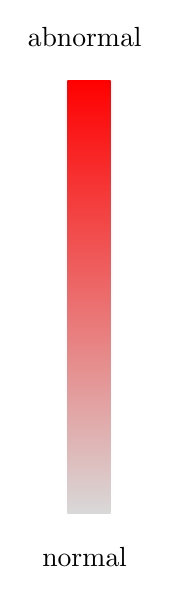
\begin{tikzpicture}[scale=1.1,auto,swap]
    \shade[top color=red,bottom color=gray!30] (0,0) rectangle (0.5,5);
    \node[inner sep=0] (corr_text) at (0.2,5.5) {abnormal};
    \node[inner sep=0] (corr_text) at (0.2,-0.5) {normal};
  \end{tikzpicture}
  \caption{}
  \label{fig:SnapEBMPCAa}
  \end{subfigure}
  
  \begin{subfigure}{1\textwidth}
  \centering
  \includegraphics[scale=0.6]{\snapLocationPCA/../patientStages.eps}
  \caption{}
  \label{fig:SnapEBMPCAb}
  \end{subfigure}

  \captionSnapEBMPCA
  
\end{figure}




\subsection{Discussion}

The EBM abnormality ordering confirms our original hypothesis, where showing that posterior regions such as occipital and superior parietal areas are the earliest to become abnormal, followed by temporal areas and inferior parietal. Moreover, in the staging histogram most controls are placed at stage zero, suggesting they have no abnormalities while PCA subjects are spread across the other stages. 

\section{AD Analysis}
\label{ebm:ad}

% \subsection{Background}
% Summarise what has been reported so far in the literature
%TODO

\subsection{Hypothesis}

In a similar way to \ref{ebm:pca}, we are interested to find out the progression of tAD using the event-based model. Previous literature has shown that the hippocampus, entorhinal cortex and other temporal areas are the first brain regions to become affected in AD \cite{braak1991neuropathological,convit1995hippocampal,xu2000usefulness}. We are interested to test this hypothesis and further find out a fine-grained picture of progression in typical AD.  

\subsection{Method}
\label{ebm:adMethod}

For doing this analysis, we used the EBM on the healthy control and tAD data from the DRC dataset. The method is exactly the same as the PCA analysis described in section \ref{ebm:pcaMethod}. 


\subsection{Results}

The results for the tAD progression are shown in Fig. \ref{fig:SnapEBMAD}. In subfigure \ref{fig:SnapEBMADa} we show the order in which cortical brain regions are affected at several stages of the EBM, according to our model. White regions are not yet affected while red regions are affected at the corresponding stage. The model assumes that all regions will eventually be affected by the disease. Moreover, in subfigure \ref{fig:SnapEBMADb} we show the histogram of EBM stages for controls and tAD subjects. 

\newcommand*{\snapLocationAD}{images/ebm/mriAllGaussUnifDirAD/snapshots} % or ../code/figures/mriAllGaussUnifDirPCA/snapshots
\newcommand*{\captionSnapEBMAD}{\caption{(a) Timing of atrophy in AD subjects according to the Event-based Model. White regions have not been affected, while red regions have been affected by the corresponding stage. (b) The histogram of EBM stages for controls and AD subjects.}\label{fig:SnapEBMAD}}


%col{x}{y}{z} respresents the color for ball z from matrix x at stage y (matrix x, stage y, ball z)
 
\definecolor{light-gray}{gray}{0.6}
\begin{figure}

  \begin{subfigure}{\textwidth}
  \centering
  %\begin{subfigure}[b]{0.15\textwidth}
    \begin{tikzpicture}[scale=1.0,auto,swap]

    % the two brain figures on top
    \node (upper_brain) at (0,1.5) { \includegraphics*[scale=\scaleBrainImg,trim=0 0 240 0]{\snapLocationAD/stage_8.eps}};
    \node (lower_brain) at (0,-1.5) { \includegraphics*[scale=\scaleBrainImg,trim=240 0 0 0]{\snapLocationAD/stage_8.eps}};
    \node[above=0cm of upper_brain] (stage) {Stage 8};
    % the balls
    
    \end{tikzpicture}
  %\end{subfigure}
  % next subfigure
  \hspace{-1.5em}
  ~
  %\begin{subfigure}[b]{0.15\textwidth}
    \begin{tikzpicture}[scale=1.0,auto,swap]

    % the two brain figures on top
    \node (upper_brain) at (0,1.5) { \includegraphics*[scale=\scaleBrainImg,trim=0 0 240 0]{\snapLocationAD/stage_16.eps}};
    \node (lower_brain) at (0,-1.5) { \includegraphics*[scale=\scaleBrainImg,trim=240 0 0 0]{\snapLocationAD/stage_16.eps}};
    \node[above=0cm of upper_brain] (stage) {Stage 16};
    % the balls
    
    \end{tikzpicture}
  %\end{subfigure}
  % next subfigure
  \hspace{-1.5em}
  ~
  %\begin{subfigure}[b]{0.15\textwidth}
    \begin{tikzpicture}[scale=1.0,auto,swap]

    % the two brain figures on top
    \node (upper_brain) at (0,1.5) { \includegraphics*[scale=\scaleBrainImg,trim=0 0 240 0]{\snapLocationAD/stage_24.eps}};
    \node (lower_brain) at (0,-1.5) { \includegraphics*[scale=\scaleBrainImg,trim=240 0 0 0]{\snapLocationAD/stage_24.eps}};
    \node[above=0cm of upper_brain] (stage) {Stage 24};
    % the balls
    
    \end{tikzpicture}
  %\end{subfigure}
  % next subfigure
  \hspace{-1.5em}
  ~
  %\begin{subfigure}[b]{0.15\textwidth}
    \begin{tikzpicture}[scale=1.0,auto,swap]

    % the two brain figures on top
    \node (upper_brain) at (0,1.5) { \includegraphics*[scale=\scaleBrainImg,trim=0 0 240 0]{\snapLocationAD/stage_32.eps}};
    \node (lower_brain) at (0,-1.5) { \includegraphics*[scale=\scaleBrainImg,trim=240 0 0 0]{\snapLocationAD/stage_32.eps}};
    \node[above=0cm of upper_brain] (stage) {Stage 32};
    % the balls
    
    \end{tikzpicture}
  %\end{subfigure}
  % next subfigure
  \hspace{-1.5em}
  ~
  %\begin{subfigure}[b]{0.15\textwidth}
    \begin{tikzpicture}[scale=1.0,auto,swap]

    % the two brain figures on top
    \node (upper_brain) at (0,1.5) { \includegraphics*[scale=\scaleBrainImg,trim=0 0 240 0]{\snapLocationAD/stage_40.eps}};
    \node (lower_brain) at (0,-1.5) { \includegraphics*[scale=\scaleBrainImg,trim=240 0 0 0]{\snapLocationAD/stage_40.eps}};
    \node[above=0cm of upper_brain] (stage) {Stage 40};
    % the balls
    
    \end{tikzpicture}
  %\end{subfigure}
  % next subfigure
  \hspace{-1.5em}
  ~
  \hspace{1em}
  % the red-to-yellow gradient on the right
  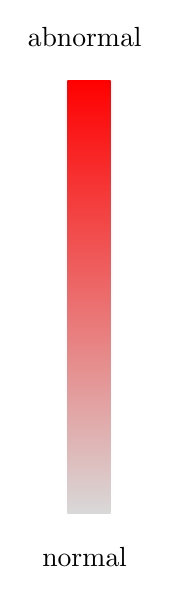
\begin{tikzpicture}[scale=1.1,auto,swap]
    \shade[top color=red,bottom color=gray!30] (0,0) rectangle (0.5,5);
    \node[inner sep=0] (corr_text) at (0.2,5.5) {abnormal};
    \node[inner sep=0] (corr_text) at (0.2,-0.5) {normal};
  \end{tikzpicture}
  \caption{}
  \label{fig:SnapEBMADa}
  \end{subfigure}
  
  \begin{subfigure}{1\textwidth}
  \centering
  \includegraphics[scale=0.6]{\snapLocationAD/../patientStages.eps}
  \caption{}
  \label{fig:SnapEBMADb}
  \end{subfigure}

  \captionSnapEBMAD
  
\end{figure}




\subsection{Discussion}
The tAD progression obtained by our data-driven model confirms previous patterns of atrophy, where the hippocampus, entorhinal, amygdala (not shown) are the earliest regions to become abnormal on in the disease time course. This is followed by other regions in this order: inferior and middle temporal regions, occipital regions, angular gyrus, precuneus and ventricles. The patient staging histogram also shows that controls are mostly at stage zero (no abnormal regions), while patients are spread across the disease stages.

\section{PCA subgroups}
\label{ebm:pca_subgroups}

\subsection{Background}

% Summarise what has been reported so far in the literature
Although PCA is considered a homogeneous disease, there have been claims in past literature that there exist three main subgroups\cite{lehmann2011basic}: parietal (dorsal) and occipitotemporal (ventral) forms of PCA have been reported by Ross et al. \cite{ross1996progressive}, while a third primary visual (striate cortex, caudal) form of PCA has been proposed by Galton et al. \cite{galton2000atypical}. In this section we are interested to analyse and compare the progression of these different subgroups. 

We split our dataset into three groups based on performance on a suite of cognitive tests. For each subject we computed the following composite tests by summing up scores from individual tests:
\begin{enumerate}
 \item Early visual processing: shape discrimination, figure-ground discrimination and simple crowding
 \item Visuoperceptual processing: object decision, fragmented letters and usual and unusual views.
 \item Visuospatial processing: number location, dot counting and a cancellation time (cut off at 90s)
 \item Episodic memory: short recognition memory test (sRMT) for words and sRMT for faces
\end{enumerate}
We then classified the subjects into three groups. The worst 1/3 of subjects on the early visual processing tests as compared to the memory tests (i.e. difference between early visual and memory tests) were assigned to the \emph{vision subgroup}. The remaining 2/3 of participants were split into two groups according to a worse performance on the visuoperceptual or visuospatial tests. More precisely, the difference between visuoperceptual and visuospatial was computed and the top half of participants was assigned to the \emph{spatial subgroup}, while the bottom half was assigned to the \emph{object subgroup}. Detailed demographics for the three PCA subgroups are shown in table \ref{tab:subgroup_demographics}.

\begin{table}
\centering
\begin{tabular}{ c |C{1.7cm} | C{1.7cm} | C{2.5cm} | C{2.5cm} | C{2.5cm}} 
\textbf{Subgroup} & \textbf{Number of Subjects} & \textbf{Gender} \hspace{1cm} M/F & \textbf{Age at baseline} \hspace{1cm} (years, mean $\pm$ std) & \textbf{Years from onset} (years, mean $\pm$ std) & \textbf{Number of scans} (mean $\pm$ std)\\
\textbf{Vision} & 23 & 6/17 & 64.4 $\pm$ 7.7 & 4.5 $\pm$ 2.8 & 2.2 $\pm$ 1.1\\ 
\textbf{Space} & 21 & 10/11 & 62.0 $\pm$ 6.8 & 4.4 $\pm$ 2.8 & 2.4 $\pm$ 1.4\\ 
\textbf{Object} & 18 & 7/11 & 62.3 $\pm$ 8.2 & 4.5 $\pm$ 2.7 & 2.7 $\pm$ 1.6\\ 
\end{tabular}
\caption[Baseline population demographics for PCA subgroups]{Baseline population demographics for PCA subgroups.}
\label{tab:subgroup_demographics}
\end{table}
 
\subsection{Hypotheses}

We formulate the following hypotheses, based on evidence from previous research\cite{ross1996progressive,galton2000atypical}:
\begin{itemize}
 \item \emph{Vision subgroup}: atrophy starts in the occipital lobe
 \item \emph{Space subgroup}: atrophy starts in the superior parietal lobe
 \item \emph{Object subgroup}: atrophy starts in the inferior temporal lobe
\end{itemize}

\subsection{Method}

We ran the EBM on data from each of the three subgroups separately, along with the shared healthy controls population. We used the same method as in the PCA analysis described in section \ref{ebm:pcaMethod}. The only difference is that we increased the range of the uniform distribution to make it span a wider interval. This was done because, due to the use of a gaussian and uniform mixture of distributions, some controls with "very good" biomarker values would be assigned to the abnormal group and subsequently later stages. Therefore, for each of the groups (\emph{vision}, \emph{space}, \emph{object}), we multiplied the initial range of the uniform distribution by a factor of 2,5 and 1 respectively.

\subsection{Results}


The positional variance matrix for the three subgroups (\emph{vision}, \emph{space}, \emph{object}) are shown in figures \ref{fig:EAR}, \ref{fig:SPA} and \ref{fig:PER} respectively. On the y-axis, we show the biomarkers representing ROI volumes ordered according to the maximum likelihood sequence $S$ from Eq. \ref{eq:ebm4}, while on the x-axis we show the position at which they become abnormal in the sequence. Each gray square at position $(i,j)$ gives the probability that biomarker $i$ is placed on position $j$ in the sequence, ranging from 0 (white cells) and to 1 (black cells).

\subsection{Discussion}

For the \emph{vision subgroup}, our hypothesis is confirmed, as the EBM suggests that the superior occipital, occipital fusiform and inferior occipital areas are the first to be affected (in no particular order). This is followed by the whole brain and parietal areas (superior parietal and precuneus). This is further followed by angular, middle occipital and middle temporal. 

In the \emph{space subgroup}, we find that the superior parietal lobe and the inferior occipital gyrus become abnormal first, again confirming our initial hypothesis. This is then followed by atrophy in the middle occipital, middle temporal, occipital fusiform and angular regions. Moreover, atrophy in the whole brain becomes detectable at this stage. 

In the \emph{object subgroup}, we find that the first two regions to become affected are the inferior occipital gyrus and the ventricles, which does not match out initial hypothesis that the inferior temporal region is affected at the very beginning. However, the inferior temporal regions is affected right after, which is still early on in the sequence. The fact that the occipital regions are also affected in this subgroup was also confirmed by previous studies \cite{ross1996progressive,kiyosawa1989alzheimer}. 


% slightly better with higher delta ... frontal went to the end but supramarginal is still at the beginning.
\begin{figure}[H]
 \centering
%  \hspace{-2.5cm}
 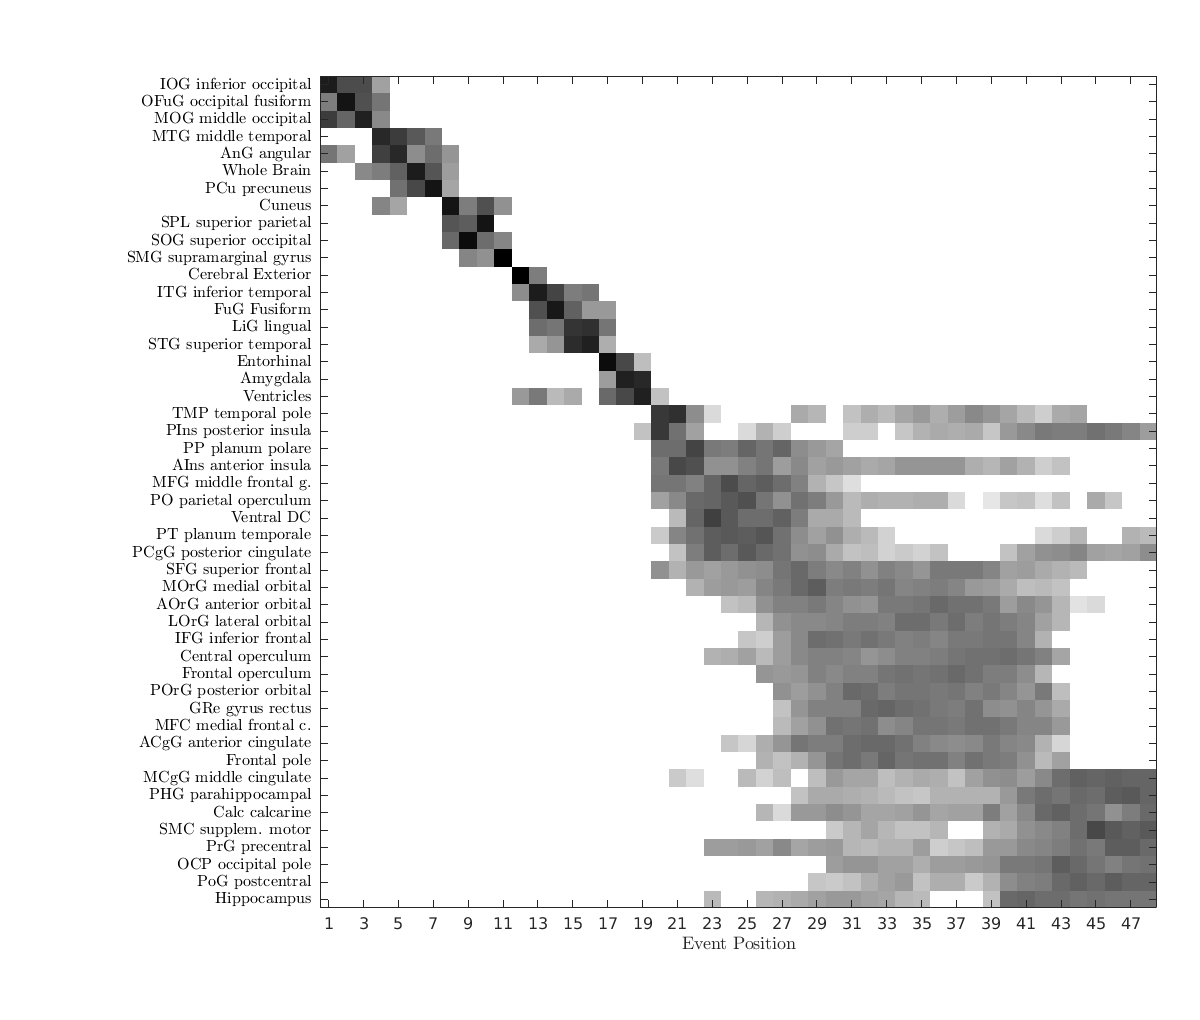
\includegraphics[scale=0.4, trim=100 50 0 0]{images/ebm/mriAllGaussUnifDirEAR/posVarianceMatrix.png}
 \caption{Positional variance matrix for the \emph{vision subgroup}. On the y-axis, we show the biomarkers representing ROI volumes ordered according to the maximum likelihood sequence, while on the x-axis we show the position at which they become abnormal in the sequence. Each gray square at position $(i,j)$ gives the probability that biomarker $i$ is placed on position $j$ in the sequence, ranging from 0 (white cells) and to 1 (black cells). Our initial hypothesis was that atrophy starts in the occipital lobe, which is confirmed by the EBM analysis.}
   \label{fig:EAR}
\end{figure}

\newcommand*{\snapLocationEAR}{images/ebm/mriAllGaussUnifDirEAR/snapshots}
\newcommand*{\captionSnapEBMEAR}{\caption{(a) Timing of atrophy for the \emph{vision} subgroup. White regions have not been affected, while red regions have been affected by the corresponding stage.}\label{fig:SnapEBMEAR}}

 
\definecolor{light-gray}{gray}{0.6}
\begin{figure}[H]
  \centering
  %\begin{subfigure}[b]{0.15\textwidth}
    \begin{tikzpicture}[scale=1.0,auto,swap]

    % the two brain figures on top
    \node (upper_brain) at (0,1.5) { \includegraphics*[scale=\scaleBrainImg,trim=0 0 240 0]{\snapLocationEAR/stage_1.eps}};
    \node (lower_brain) at (0,-1.5) { \includegraphics*[scale=\scaleBrainImg,trim=240 0 0 0]{\snapLocationEAR/stage_1.eps}};
    \node[above=0cm of upper_brain] (stage) {Stage 1};
    % the balls
    
    \end{tikzpicture}
  %\end{subfigure}
  % next subfigure
  \hspace{-1.5em}
  ~
  %\begin{subfigure}[b]{0.15\textwidth}
    \begin{tikzpicture}[scale=1.0,auto,swap]

    % the two brain figures on top
    \node (upper_brain) at (0,1.5) { \includegraphics*[scale=\scaleBrainImg,trim=0 0 240 0]{\snapLocationEAR/stage_2.eps}};
    \node (lower_brain) at (0,-1.5) { \includegraphics*[scale=\scaleBrainImg,trim=240 0 0 0]{\snapLocationEAR/stage_2.eps}};
    \node[above=0cm of upper_brain] (stage) {Stage 2};
    % the balls
    
    \end{tikzpicture}
  %\end{subfigure}
  % next subfigure
  \hspace{-1.5em}
  ~
  %\begin{subfigure}[b]{0.15\textwidth}
    \begin{tikzpicture}[scale=1.0,auto,swap]

    % the two brain figures on top
    \node (upper_brain) at (0,1.5) { \includegraphics*[scale=\scaleBrainImg,trim=0 0 240 0]{\snapLocationEAR/stage_3.eps}};
    \node (lower_brain) at (0,-1.5) { \includegraphics*[scale=\scaleBrainImg,trim=240 0 0 0]{\snapLocationEAR/stage_3.eps}};
    \node[above=0cm of upper_brain] (stage) {Stage 3};
    % the balls
    
    \end{tikzpicture}
  %\end{subfigure}
  % next subfigure
  \hspace{-1.5em}
  ~
  %\begin{subfigure}[b]{0.15\textwidth}
    \begin{tikzpicture}[scale=1.0,auto,swap]

    % the two brain figures on top
    \node (upper_brain) at (0,1.5) { \includegraphics*[scale=\scaleBrainImg,trim=0 0 240 0]{\snapLocationEAR/stage_4.eps}};
    \node (lower_brain) at (0,-1.5) { \includegraphics*[scale=\scaleBrainImg,trim=240 0 0 0]{\snapLocationEAR/stage_4.eps}};
    \node[above=0cm of upper_brain] (stage) {Stage 4};
    % the balls
    
    \end{tikzpicture}
  %\end{subfigure}
  % next subfigure
  \hspace{-1.5em}
  ~
  %\begin{subfigure}[b]{0.15\textwidth}
    \begin{tikzpicture}[scale=1.0,auto,swap]

    % the two brain figures on top
    \node (upper_brain) at (0,1.5) { \includegraphics*[scale=\scaleBrainImg,trim=0 0 240 0]{\snapLocationEAR/stage_5.eps}};
    \node (lower_brain) at (0,-1.5) { \includegraphics*[scale=\scaleBrainImg,trim=240 0 0 0]{\snapLocationEAR/stage_5.eps}};
    \node[above=0cm of upper_brain] (stage) {Stage 5};
    % the balls
    
    \end{tikzpicture}
  %\end{subfigure}
  % next subfigure
  \hspace{-1.5em}
  ~
  %\begin{subfigure}[b]{0.15\textwidth}
    \begin{tikzpicture}[scale=1.0,auto,swap]

    % the two brain figures on top
    \node (upper_brain) at (0,1.5) { \includegraphics*[scale=\scaleBrainImg,trim=0 0 240 0]{\snapLocationEAR/stage_6.eps}};
    \node (lower_brain) at (0,-1.5) { \includegraphics*[scale=\scaleBrainImg,trim=240 0 0 0]{\snapLocationEAR/stage_6.eps}};
    \node[above=0cm of upper_brain] (stage) {Stage 6};
    % the balls
    
    \end{tikzpicture}
  %\end{subfigure}
  % next subfigure
  \hspace{-1.5em}
  ~
  %\begin{subfigure}[b]{0.15\textwidth}
    \begin{tikzpicture}[scale=1.0,auto,swap]

    % the two brain figures on top
    \node (upper_brain) at (0,1.5) { \includegraphics*[scale=\scaleBrainImg,trim=0 0 240 0]{\snapLocationEAR/stage_7.eps}};
    \node (lower_brain) at (0,-1.5) { \includegraphics*[scale=\scaleBrainImg,trim=240 0 0 0]{\snapLocationEAR/stage_7.eps}};
    \node[above=0cm of upper_brain] (stage) {Stage 7};
    % the balls
    
    \end{tikzpicture}
  %\end{subfigure}
  % next subfigure
  \hspace{-1.5em}
  ~
  %\begin{subfigure}[b]{0.15\textwidth}
    \begin{tikzpicture}[scale=1.0,auto,swap]

    % the two brain figures on top
    \node (upper_brain) at (0,1.5) { \includegraphics*[scale=\scaleBrainImg,trim=0 0 240 0]{\snapLocationEAR/stage_8.eps}};
    \node (lower_brain) at (0,-1.5) { \includegraphics*[scale=\scaleBrainImg,trim=240 0 0 0]{\snapLocationEAR/stage_8.eps}};
    \node[above=0cm of upper_brain] (stage) {Stage 8};
    % the balls
    
    \end{tikzpicture}
  %\end{subfigure}
  % next subfigure
  \hspace{-1.5em}
  ~
  %\begin{subfigure}[b]{0.15\textwidth}
    \begin{tikzpicture}[scale=1.0,auto,swap]

    % the two brain figures on top
    \node (upper_brain) at (0,1.5) { \includegraphics*[scale=\scaleBrainImg,trim=0 0 240 0]{\snapLocationEAR/stage_9.eps}};
    \node (lower_brain) at (0,-1.5) { \includegraphics*[scale=\scaleBrainImg,trim=240 0 0 0]{\snapLocationEAR/stage_9.eps}};
    \node[above=0cm of upper_brain] (stage) {Stage 9};
    % the balls
    
    \end{tikzpicture}
  %\end{subfigure}
  % next subfigure
  \hspace{-1.5em}
  ~
  \hspace{1em}
  % the red-to-yellow gradient on the right
  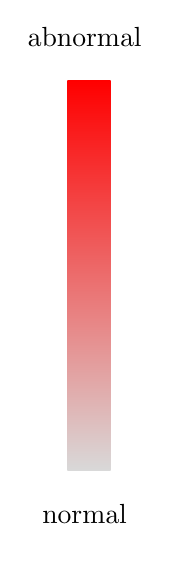
\begin{tikzpicture}[scale=1.1,auto,swap]
    \shade[top color=red,bottom color=gray!30] (0,1.5) rectangle (0.5,6);
    \node[inner sep=0] (corr_text) at (0.2,6.5) {abnormal};
    \node[inner sep=0] (corr_text) at (0.2,1) {normal};
    \node[inner sep=0] (corr_text) at (0.2,0.5) {};
  \end{tikzpicture}
  \captionSnapEBMEAR
\end{figure}





% \pagebreak

% superior parietal went earlier with around 4 positions, but still on place 4
\begin{figure}[H]
 \centering
%  \hspace{-2.5cm}
 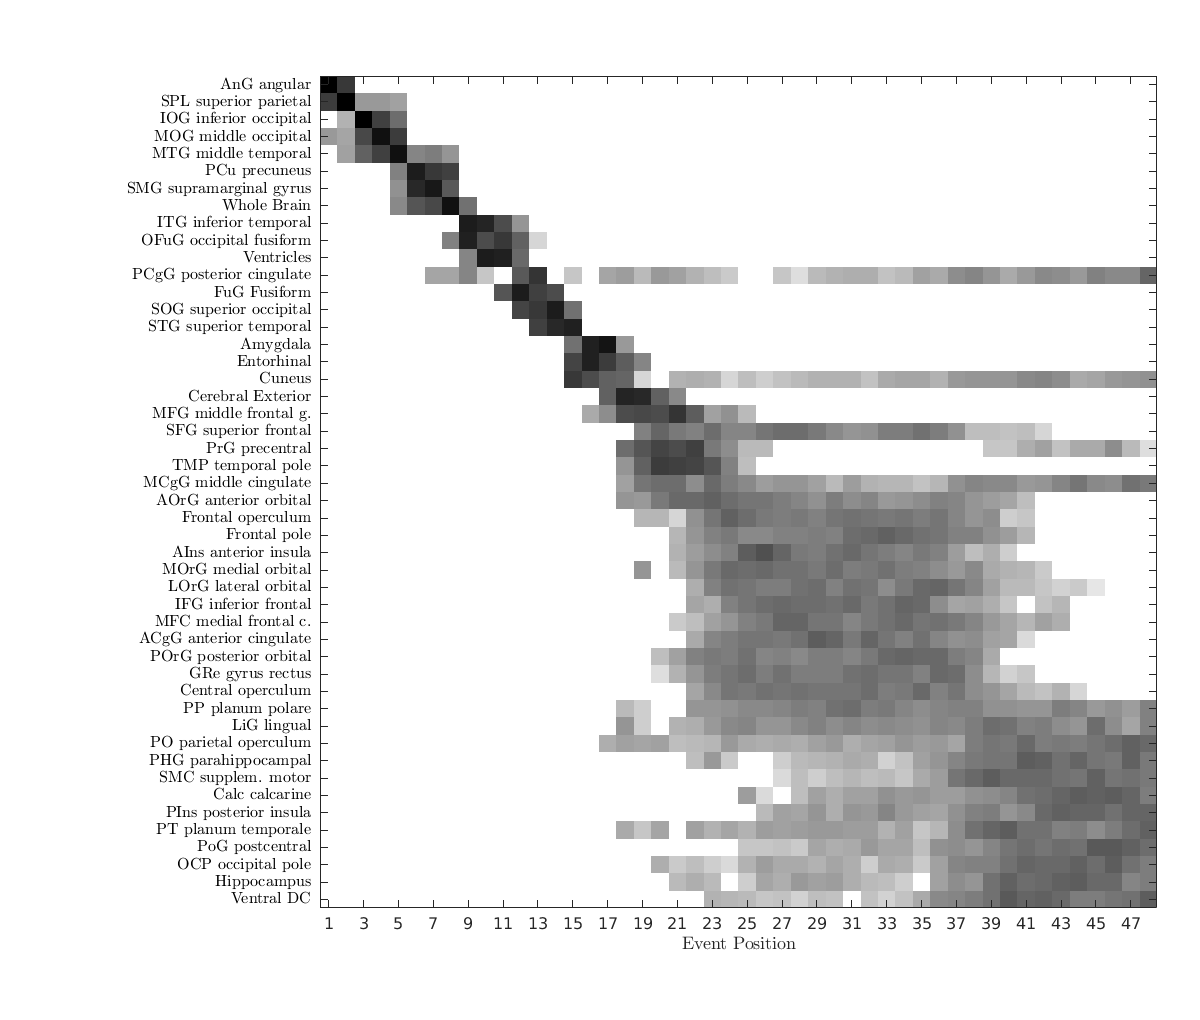
\includegraphics[scale=0.4, trim=100 50 0 0]{images/ebm/mriAllGaussUnifDirSPA/posVarianceMatrix.png}
 \caption{Positional variance matrix for the \emph{space subgroup}. On the y-axis, we show the biomarkers representing ROI volumes ordered according to the maximum likelihood sequence, while on the x-axis we show the position at which they become abnormal in the sequence. Each gray square at position $(i,j)$ gives the probability that biomarker $i$ is placed on position $j$ in the sequence, ranging from 0 (white cells) and to 1 (black cells). Our initial hypothesis was that atrophy starts in the superior parietal lobe. This is confirmed by the EBM analysis, which suggests atrophy starts in the angular and superior parietal regions.}
   \label{fig:SPA}
\end{figure}

\newcommand*{\snapLocationSPA}{images/ebm/mriAllGaussUnifDirSPA/snapshots} 
\newcommand*{\captionSnapEBMSPA}{\caption{(a) Timing of atrophy for the \emph{space} subgroup. White regions have not been affected, while red regions have been affected by the corresponding stage.}\label{fig:SnapEBMSPA}}


 
\definecolor{light-gray}{gray}{0.6}
\begin{figure}[H]
  \centering
  %\begin{subfigure}[b]{0.15\textwidth}
    \begin{tikzpicture}[scale=1.0,auto,swap]

    % the two brain figures on top
    \node (upper_brain) at (0,1.5) { \includegraphics*[scale=\scaleBrainImg,trim=0 0 240 0]{\snapLocationSPA/stage_1.eps}};
    \node (lower_brain) at (0,-1.5) { \includegraphics*[scale=\scaleBrainImg,trim=240 0 0 0]{\snapLocationSPA/stage_1.eps}};
    \node[above=0cm of upper_brain] (stage) {Stage 1};
    % the balls
    
    \end{tikzpicture}
  %\end{subfigure}
  % next subfigure
  \hspace{-1.5em}
  ~
  %\begin{subfigure}[b]{0.15\textwidth}
    \begin{tikzpicture}[scale=1.0,auto,swap]

    % the two brain figures on top
    \node (upper_brain) at (0,1.5) { \includegraphics*[scale=\scaleBrainImg,trim=0 0 240 0]{\snapLocationSPA/stage_2.eps}};
    \node (lower_brain) at (0,-1.5) { \includegraphics*[scale=\scaleBrainImg,trim=240 0 0 0]{\snapLocationSPA/stage_2.eps}};
    \node[above=0cm of upper_brain] (stage) {Stage 2};
    % the balls
    
    \end{tikzpicture}
  %\end{subfigure}
  % next subfigure
  \hspace{-1.5em}
  ~
  %\begin{subfigure}[b]{0.15\textwidth}
    \begin{tikzpicture}[scale=1.0,auto,swap]

    % the two brain figures on top
    \node (upper_brain) at (0,1.5) { \includegraphics*[scale=\scaleBrainImg,trim=0 0 240 0]{\snapLocationSPA/stage_3.eps}};
    \node (lower_brain) at (0,-1.5) { \includegraphics*[scale=\scaleBrainImg,trim=240 0 0 0]{\snapLocationSPA/stage_3.eps}};
    \node[above=0cm of upper_brain] (stage) {Stage 3};
    % the balls
    
    \end{tikzpicture}
  %\end{subfigure}
  % next subfigure
  \hspace{-1.5em}
  ~
  %\begin{subfigure}[b]{0.15\textwidth}
    \begin{tikzpicture}[scale=1.0,auto,swap]

    % the two brain figures on top
    \node (upper_brain) at (0,1.5) { \includegraphics*[scale=\scaleBrainImg,trim=0 0 240 0]{\snapLocationSPA/stage_4.eps}};
    \node (lower_brain) at (0,-1.5) { \includegraphics*[scale=\scaleBrainImg,trim=240 0 0 0]{\snapLocationSPA/stage_4.eps}};
    \node[above=0cm of upper_brain] (stage) {Stage 4};
    % the balls
    
    \end{tikzpicture}
  %\end{subfigure}
  % next subfigure
  \hspace{-1.5em}
  ~
  %\begin{subfigure}[b]{0.15\textwidth}
    \begin{tikzpicture}[scale=1.0,auto,swap]

    % the two brain figures on top
    \node (upper_brain) at (0,1.5) { \includegraphics*[scale=\scaleBrainImg,trim=0 0 240 0]{\snapLocationSPA/stage_5.eps}};
    \node (lower_brain) at (0,-1.5) { \includegraphics*[scale=\scaleBrainImg,trim=240 0 0 0]{\snapLocationSPA/stage_5.eps}};
    \node[above=0cm of upper_brain] (stage) {Stage 5};
    % the balls
    
    \end{tikzpicture}
  %\end{subfigure}
  % next subfigure
  \hspace{-1.5em}
  ~
  %\begin{subfigure}[b]{0.15\textwidth}
    \begin{tikzpicture}[scale=1.0,auto,swap]

    % the two brain figures on top
    \node (upper_brain) at (0,1.5) { \includegraphics*[scale=\scaleBrainImg,trim=0 0 240 0]{\snapLocationSPA/stage_6.eps}};
    \node (lower_brain) at (0,-1.5) { \includegraphics*[scale=\scaleBrainImg,trim=240 0 0 0]{\snapLocationSPA/stage_6.eps}};
    \node[above=0cm of upper_brain] (stage) {Stage 6};
    % the balls
    
    \end{tikzpicture}
  %\end{subfigure}
  % next subfigure
  \hspace{-1.5em}
  ~
  %\begin{subfigure}[b]{0.15\textwidth}
    \begin{tikzpicture}[scale=1.0,auto,swap]

    % the two brain figures on top
    \node (upper_brain) at (0,1.5) { \includegraphics*[scale=\scaleBrainImg,trim=0 0 240 0]{\snapLocationSPA/stage_7.eps}};
    \node (lower_brain) at (0,-1.5) { \includegraphics*[scale=\scaleBrainImg,trim=240 0 0 0]{\snapLocationSPA/stage_7.eps}};
    \node[above=0cm of upper_brain] (stage) {Stage 7};
    % the balls
    
    \end{tikzpicture}
  %\end{subfigure}
  % next subfigure
  \hspace{-1.5em}
  ~
  %\begin{subfigure}[b]{0.15\textwidth}
    \begin{tikzpicture}[scale=1.0,auto,swap]

    % the two brain figures on top
    \node (upper_brain) at (0,1.5) { \includegraphics*[scale=\scaleBrainImg,trim=0 0 240 0]{\snapLocationSPA/stage_8.eps}};
    \node (lower_brain) at (0,-1.5) { \includegraphics*[scale=\scaleBrainImg,trim=240 0 0 0]{\snapLocationSPA/stage_8.eps}};
    \node[above=0cm of upper_brain] (stage) {Stage 8};
    % the balls
    
    \end{tikzpicture}
  %\end{subfigure}
  % next subfigure
  \hspace{-1.5em}
  ~
  %\begin{subfigure}[b]{0.15\textwidth}
    \begin{tikzpicture}[scale=1.0,auto,swap]

    % the two brain figures on top
    \node (upper_brain) at (0,1.5) { \includegraphics*[scale=\scaleBrainImg,trim=0 0 240 0]{\snapLocationSPA/stage_9.eps}};
    \node (lower_brain) at (0,-1.5) { \includegraphics*[scale=\scaleBrainImg,trim=240 0 0 0]{\snapLocationSPA/stage_9.eps}};
    \node[above=0cm of upper_brain] (stage) {Stage 9};
    % the balls
    
    \end{tikzpicture}
  %\end{subfigure}
  % next subfigure
  \hspace{-1.5em}
  ~
  \hspace{1em}
  % the red-to-yellow gradient on the right
  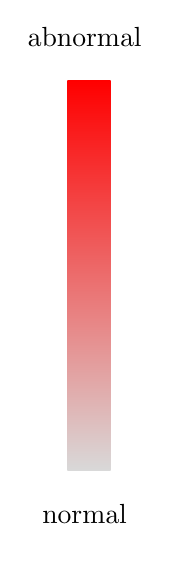
\begin{tikzpicture}[scale=1.1,auto,swap]
    \shade[top color=red,bottom color=gray!30] (0,1.5) rectangle (0.5,6);
    \node[inner sep=0] (corr_text) at (0.2,6.5) {abnormal};
    \node[inner sep=0] (corr_text) at (0.2,1) {normal};
    \node[inner sep=0] (corr_text) at (0.2,0.5) {};
  \end{tikzpicture}
  \captionSnapEBMSPA
\end{figure}





% \pagebreak

\begin{figure}[H]
 \centering
%  \hspace{-2.5cm}
 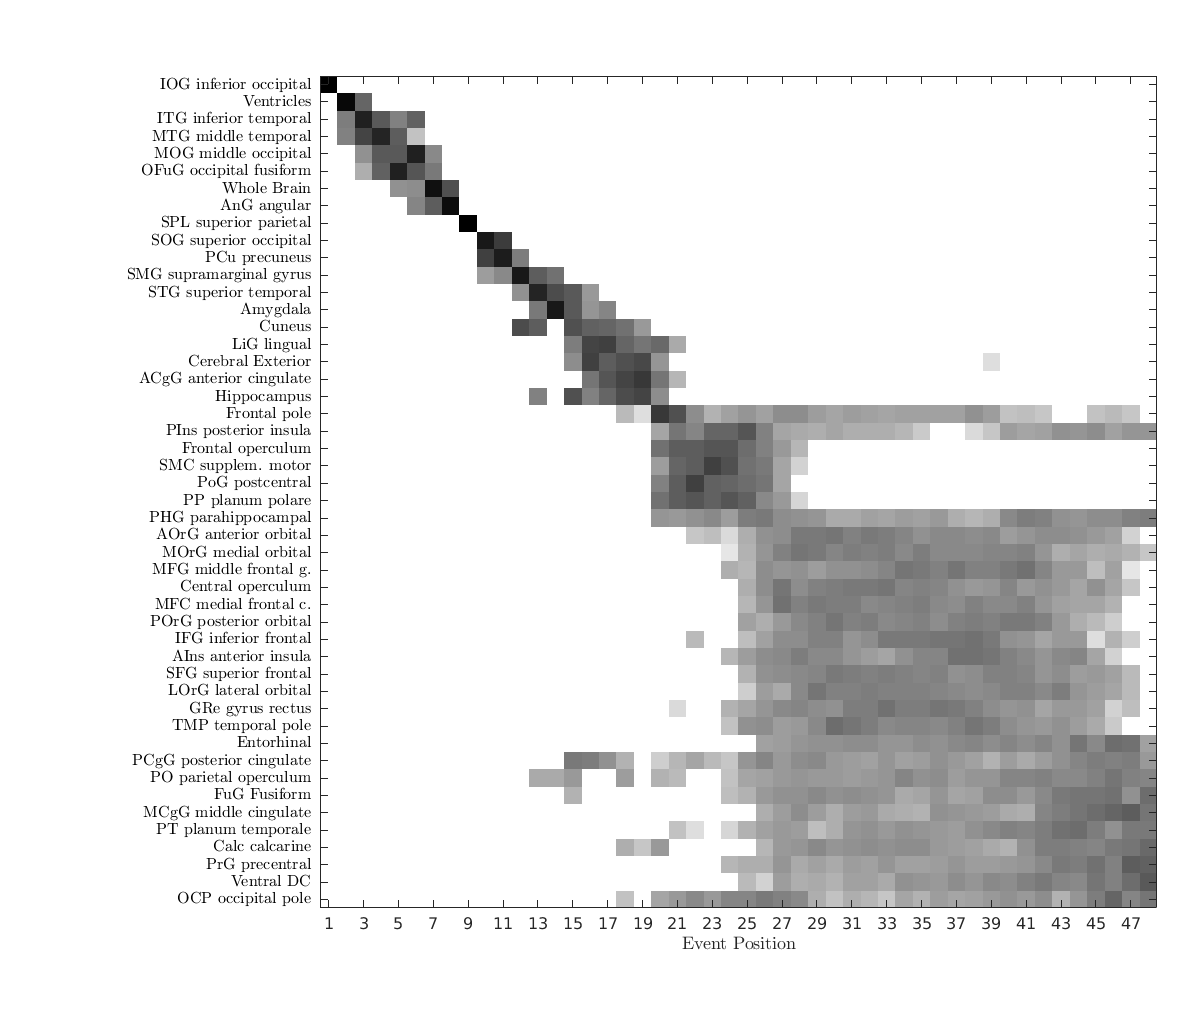
\includegraphics[scale=0.4, trim=100 50 0 0]{images/ebm/mriAllGaussUnifDirPER/posVarianceMatrix.png}
 \caption{Positional variance matrix for the \emph{object subgroup}. On the y-axis, we show the biomarkers representing ROI volumes ordered according to the maximum likelihood sequence, while on the x-axis we show the position at which they become abnormal in the sequence. Each gray square at position $(i,j)$ gives the probability that biomarker $i$ is placed on position $j$ in the sequence, ranging from 0 (white cells) and to 1 (black cells). Our initial hypothesis was that atrophy starts in the inferior temporal lobe, which is not confirmed by the EBM analysis as the inferior temporal region becomes abnormal only after the inferior occipital and ventricles.}
   \label{fig:PER}
\end{figure}

\newcommand*{\snapLocationPER}{images/ebm/mriAllGaussUnifDirPER/snapshots} % 
\newcommand*{\captionSnapEBMPER}{\caption{(a) Timing of atrophy for the \emph{object} subgroup. White regions have not been affected, while red regions have been affected by the corresponding stage.}\label{fig:SnapEBMPER}}


 
\definecolor{light-gray}{gray}{0.6}
\begin{figure}[H]
  \centering
  %\begin{subfigure}[b]{0.15\textwidth}
    \begin{tikzpicture}[scale=1.0,auto,swap]

    % the two brain figures on top
    \node (upper_brain) at (0,1.5) { \includegraphics*[scale=\scaleBrainImg,trim=0 0 240 0]{\snapLocationPER/stage_1.eps}};
    \node (lower_brain) at (0,-1.5) { \includegraphics*[scale=\scaleBrainImg,trim=240 0 0 0]{\snapLocationPER/stage_1.eps}};
    \node[above=0cm of upper_brain] (stage) {Stage 1};
    % the balls
    
    \end{tikzpicture}
  %\end{subfigure}
  % next subfigure
  \hspace{-1.5em}
  ~
  %\begin{subfigure}[b]{0.15\textwidth}
    \begin{tikzpicture}[scale=1.0,auto,swap]

    % the two brain figures on top
    \node (upper_brain) at (0,1.5) { \includegraphics*[scale=\scaleBrainImg,trim=0 0 240 0]{\snapLocationPER/stage_2.eps}};
    \node (lower_brain) at (0,-1.5) { \includegraphics*[scale=\scaleBrainImg,trim=240 0 0 0]{\snapLocationPER/stage_2.eps}};
    \node[above=0cm of upper_brain] (stage) {Stage 2};
    % the balls
    
    \end{tikzpicture}
  %\end{subfigure}
  % next subfigure
  \hspace{-1.5em}
  ~
  %\begin{subfigure}[b]{0.15\textwidth}
    \begin{tikzpicture}[scale=1.0,auto,swap]

    % the two brain figures on top
    \node (upper_brain) at (0,1.5) { \includegraphics*[scale=\scaleBrainImg,trim=0 0 240 0]{\snapLocationPER/stage_3.eps}};
    \node (lower_brain) at (0,-1.5) { \includegraphics*[scale=\scaleBrainImg,trim=240 0 0 0]{\snapLocationPER/stage_3.eps}};
    \node[above=0cm of upper_brain] (stage) {Stage 3};
    % the balls
    
    \end{tikzpicture}
  %\end{subfigure}
  % next subfigure
  \hspace{-1.5em}
  ~
  %\begin{subfigure}[b]{0.15\textwidth}
    \begin{tikzpicture}[scale=1.0,auto,swap]

    % the two brain figures on top
    \node (upper_brain) at (0,1.5) { \includegraphics*[scale=\scaleBrainImg,trim=0 0 240 0]{\snapLocationPER/stage_4.eps}};
    \node (lower_brain) at (0,-1.5) { \includegraphics*[scale=\scaleBrainImg,trim=240 0 0 0]{\snapLocationPER/stage_4.eps}};
    \node[above=0cm of upper_brain] (stage) {Stage 4};
    % the balls
    
    \end{tikzpicture}
  %\end{subfigure}
  % next subfigure
  \hspace{-1.5em}
  ~
  %\begin{subfigure}[b]{0.15\textwidth}
    \begin{tikzpicture}[scale=1.0,auto,swap]

    % the two brain figures on top
    \node (upper_brain) at (0,1.5) { \includegraphics*[scale=\scaleBrainImg,trim=0 0 240 0]{\snapLocationPER/stage_5.eps}};
    \node (lower_brain) at (0,-1.5) { \includegraphics*[scale=\scaleBrainImg,trim=240 0 0 0]{\snapLocationPER/stage_5.eps}};
    \node[above=0cm of upper_brain] (stage) {Stage 5};
    % the balls
    
    \end{tikzpicture}
  %\end{subfigure}
  % next subfigure
  \hspace{-1.5em}
  ~
  %\begin{subfigure}[b]{0.15\textwidth}
    \begin{tikzpicture}[scale=1.0,auto,swap]

    % the two brain figures on top
    \node (upper_brain) at (0,1.5) { \includegraphics*[scale=\scaleBrainImg,trim=0 0 240 0]{\snapLocationPER/stage_6.eps}};
    \node (lower_brain) at (0,-1.5) { \includegraphics*[scale=\scaleBrainImg,trim=240 0 0 0]{\snapLocationPER/stage_6.eps}};
    \node[above=0cm of upper_brain] (stage) {Stage 6};
    % the balls
    
    \end{tikzpicture}
  %\end{subfigure}
  % next subfigure
  \hspace{-1.5em}
  ~
  %\begin{subfigure}[b]{0.15\textwidth}
    \begin{tikzpicture}[scale=1.0,auto,swap]

    % the two brain figures on top
    \node (upper_brain) at (0,1.5) { \includegraphics*[scale=\scaleBrainImg,trim=0 0 240 0]{\snapLocationPER/stage_7.eps}};
    \node (lower_brain) at (0,-1.5) { \includegraphics*[scale=\scaleBrainImg,trim=240 0 0 0]{\snapLocationPER/stage_7.eps}};
    \node[above=0cm of upper_brain] (stage) {Stage 7};
    % the balls
    
    \end{tikzpicture}
  %\end{subfigure}
  % next subfigure
  \hspace{-1.5em}
  ~
  %\begin{subfigure}[b]{0.15\textwidth}
    \begin{tikzpicture}[scale=1.0,auto,swap]

    % the two brain figures on top
    \node (upper_brain) at (0,1.5) { \includegraphics*[scale=\scaleBrainImg,trim=0 0 240 0]{\snapLocationPER/stage_8.eps}};
    \node (lower_brain) at (0,-1.5) { \includegraphics*[scale=\scaleBrainImg,trim=240 0 0 0]{\snapLocationPER/stage_8.eps}};
    \node[above=0cm of upper_brain] (stage) {Stage 8};
    % the balls
    
    \end{tikzpicture}
  %\end{subfigure}
  % next subfigure
  \hspace{-1.5em}
  ~
  %\begin{subfigure}[b]{0.15\textwidth}
    \begin{tikzpicture}[scale=1.0,auto,swap]

    % the two brain figures on top
    \node (upper_brain) at (0,1.5) { \includegraphics*[scale=\scaleBrainImg,trim=0 0 240 0]{\snapLocationPER/stage_9.eps}};
    \node (lower_brain) at (0,-1.5) { \includegraphics*[scale=\scaleBrainImg,trim=240 0 0 0]{\snapLocationPER/stage_9.eps}};
    \node[above=0cm of upper_brain] (stage) {Stage 9};
    % the balls
    
    \end{tikzpicture}
  %\end{subfigure}
  % next subfigure
  \hspace{-1.5em}
  ~
  \hspace{1em}
  % the red-to-yellow gradient on the right
  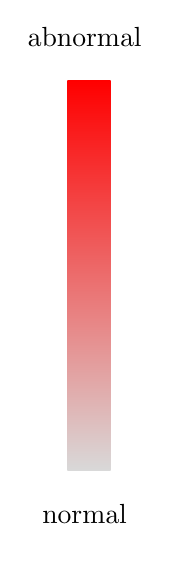
\begin{tikzpicture}[scale=1.1,auto,swap]
    \shade[top color=red,bottom color=gray!30] (0,1.5) rectangle (0.5,6);
    \node[inner sep=0] (corr_text) at (0.2,6.5) {abnormal};
    \node[inner sep=0] (corr_text) at (0.2,1) {normal};
    \node[inner sep=0] (corr_text) at (0.2,0.5) {};
  \end{tikzpicture}
  \captionSnapEBMPER
\end{figure}




\section{Conclusion}

% summary
In this chapter we showed that the EBM is a powerful tool for studying progression of typical Alzheimer disease and other subtypes. The main advantages of the model is that it does not require longitudinal data, making it especially useful for analysing rare dementias where no no large, longitudinal datasets currently exist. We have shown that the EBM results confirm patterns of atrophy previously reported in the literature, but gives a much more fine-grained picture of the temporal progression than these studies.

% limitation of the analysis (not the EBM)
The current analysis has several limitations. First of all, we assumed that the control population was well defined in order to fit the distribution of normal biomarker values directly on control data. However, the controls might show some abnormalities in CSF biomarkers, but no such data was available. Secondly, we only explored brain volumes, but other biomarkers such as cortical thickness can be further analysed using our data. 

% Future work motivated by the limitations
There are several avenues of future research. For fitting the distributions of normal and abnormal biomarker values we could use data-driven methods such as mixture model optimisation. Another option is to use the optimised EBM fitting procedures such as simultaneous sampling (section \ref{sec:simultSampling}) or Expectation-Maximisation (section \ref{sec:ebmEM}). Further analysis also needs to be done in order to answer questions related to the extent and rate of atrophy in PCA and the respective subgroups. This analysis has been done with the differential equation model in chapter \ref{chapter:diffeq}, but not at the PCA subgroup level due to the lack of sufficient longitudinal data. 



\chapter{Differential Equation Model}
\label{chapter:diffeq}

In this chapter we present a longitudinal analysis performed on the DRC data using the differential equation model (see section \ref{sec:dem}). In section \ref{sec:demClinicalQuestions} we present the clinical questions that we want to answer, in section \ref{sec:demMethod} we present the methodological details, in \ref{sec:demResults} we present the results and in \ref{sec:demDiscussion} we discuss our findings. 

% \section{Background}

% Summarise what has been reported so far in the literature
%TODO

\section{Clinical questions}
\label{sec:demClinicalQuestions}

The main questions we want to answer in this longitudinal analysis are:
\begin{enumerate}
\item In PCA, what are the differences in timing of atrophy and rates of atrophy between different brain regions? 
\item In tAD, what are the differences in timing of atrophy and rates of atrophy between different brain regions? 
\item Do people with PCA and AD lose brain volume at same speed? 
\item What are the differences in rates of atrophy across brain regions in PCA compared to AD? 
\end{enumerate}

\section{Method}
\label{sec:demMethod}

We used the differential equation model as described in section \ref{sec:dem}, where we fit a Gaussian Process (GP) to the change in biomarker scores $\Delta s / \Delta t$. The GP was fit independently for each biomarker. We used a non-parametric model such as GPs in order not to impose any parametric shape of the biomarker trajectory. Furthermore, given that the DRC dataset has a well-defined control population, we do not include the controls in the fitting of the GP as there is very little change in their biomarker values across timepoints which is not due to measurement noise. Moreover, in order to get a good fit of the GP we normalise the average biomarker values to z-scores and standardise the rates of change by dividing them with the average rate of change of all patients. The prior of the GP is kept at $Y=0$, which ensures that the trajectory has upper and lower asymptotes. 

After fitting the GP process we extracted the mean of the GP and sampled 20 trajectories from the posterior distribution of the GP in order to measure uncertainty in the model fit. The mean trajectory and trajectory samples were integrated using the numerical approach from Eq. \ref{eq:dem3}. The resulting trajectories were however not aligned on the temporal axis, since we fit the model for each biomarker independently. We therefore aligned the $t=0$ point so that $f(t=0)$ is the average biomarker value for every patient at baseline visit. More information about the alignment is give in section \ref{sec:demTrajAlignSimple}. This process was repeated independently for every mean trajectory in every biomarker. We also aligned the sampled trajectories in a similar fashion, with the only distinction that at the alignment point we added an amount of noise on the y-axis. This noise was computed as the standard deviation of the biomarker measurements for each patient at baseline visit. In order to discuss the differences in rates of atrophy across different biomarkers of diseases, we qualitatively compare the rates of atrophy at the point where the maximum rate of atrophy is attained. Moreover, a meaningful comparison of rates of atrophy across biomarkers requires them to be in a similar scale, so we converted the biomarker values representing ROI volumes to z-scores relative to controls. 

\section{Results}
\label{sec:demResults}

In Fig. \ref{fig:trajDEMPCA} we show the temporally aligned average trajectories for PCA subjects across several ROIs, while in Fig. \ref{fig:trajDEMAD} we show the trajectories for AD subjects. On the x-axis we show the number of years since baseline visit, while on the y-axis we show the z-score of the ROI volume relative to controls. The direction of the "ventricles" biomarker has been manually flipped for consistency with the other biomarkers. In Fig. \ref{trajDEMPcaAd} we show the trajectories of ROI volumes aligned for PCA and tAD along with integrated samples from the GP posterior that have been integrated and temporally aligned. The integrated posterior samples give an idea of the confidence in the average biomarker trajectory. Results from figure \ref{fig:trajDEM} can help us answer questions 1 and 2, while results from Fig. \ref{trajDEMPcaAd} can help us answer questions 3 and 4. 

\section{Discussion}
\label{sec:demDiscussion}

In the PCA progression from \ref{fig:trajDEMPCA}, in terms of timing of atrophy we find that the occipital and parietal lobes are the regions most affected early in the disease time course, before baseline visit. However, soon after baseline visit other biomarkers such as whole brain, temporal lobe and ventricles become abnormal. This matches our previous results on the same dataset using a fundamentally different model (the EBM, see section \ref{ebm:pca}), but provides more detail on the exact timing of atrophy. In terms of rates of atrophy, we see that the whole brain, ventricles and the temporal lobe are the ones showing the highest drop, which happens between baseline visit and 5 years later. While these findings confirm previous results in the literature \cite{lehmann2011cortical,whitwell2007imaging}, they provide a more detail regarding the exact timing and rate of atrophy decline over a timespan of 30 years. 

In the tAD progression from \ref{fig:trajDEMPCA}, in terms of timing of atrophy we find that the hippocampus is the first to become abnormal in the early stages, which is something that has been consistently confirmed across many other studies. Our model also predicts that in early stages the hippocampus is more sensitive than the entorhinal cortex and that the hippocampal atrophy precedes entorhinal atrophy. This has been confirmed by some previous studies \cite{laakso2000hippocampus,fonteijn2012event} but rejected by others \cite{braak1994morphological,pennanen2004hippocampus}. However, in middle and late stages we see a much more global patterns of atrophy affecting most brain areas. In terms of rate of atrophy, we find that in early stages many regions have a similar rate of decline, with only the hippocampus and ventricles showing a slightly slower rate. This is in contrast with previous findings in the literature such as \cite{scahill2002mapping} that find the hippocampus to have the highest rate of decline. We also find very similar rates especially right after the baseline visit, with slightly higher drops in volume for temporal and whole brain biomarkers.

When comparing PCA versus tAD, we find several differences in atrophy timings, rates and extent. In terms of whole brain, there is a comparable timing and rate of atrophy in both PCA and tAD in early stages, but in later stages at around baseline we find that there is more atrophy in PCA as compared to tAD. For the ROIs, we find that in PCA there is a significant amount of early and extensive atrophy in occipital and parietal areas as compared to tAD. On the other hand, in tAD there is significantly more atrophy in the hippocampus and entorhinal areas at any point in the disease, with more extensive atrophy in the hippocampus. Moreover, the hippocampus also reaches abnormal levels (-1 standard deviation) much earlier (15 to 10 years before baseline scan) in tAD compared with PCA (2 to 3 years after baseline scan). We notice that for many biomarkers sch as temporal, entorhinal and frontal there are reasonably similar rates of atrophy at many stages of the two diseases. 

\begin{figure}
\begin{subfigure}{\textwidth}
 \centering
%  \hspace{-2.5cm}
 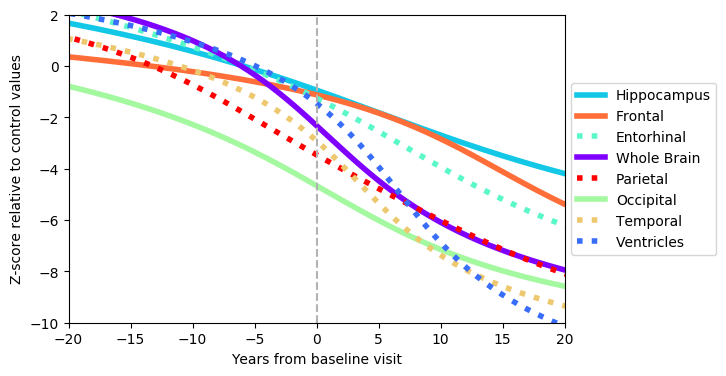
\includegraphics[scale=0.5]{images/dem/mriSmallSebPaper_DEMStdPCA_trajAlign.png}
 \caption{PCA progression}
 \label{fig:trajDEMPCA}
\end{subfigure}
\begin{subfigure}{\textwidth}
 \centering
%  \hspace{-2.5cm}
 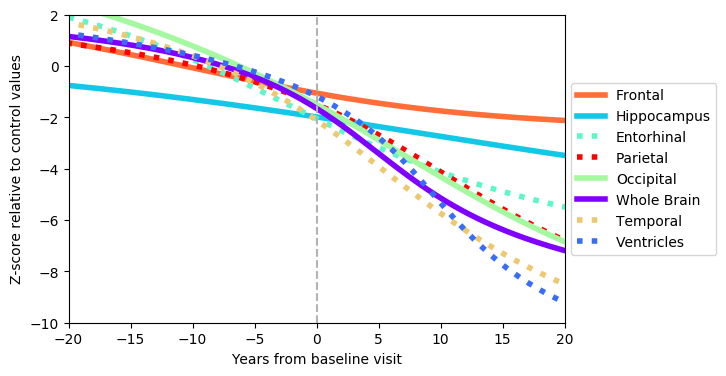
\includegraphics[scale=0.5]{images/dem/mriSmallSebPaper_DEMStdAD_trajAlign.png}
 \caption{tAD progression}
  \label{fig:trajDEMAD}
\end{subfigure}
\caption{Trajectories of different ROI volumes from the differential equation model on the (a) PCA progression and (b) tAD progression. On the x-axis we show the number of years since baseline visit, while on the y-axis we show the z-score of the ROI volume relative to controls.}
\label{fig:trajDEM}
\end{figure}

\begin{figure}
 \centering
%  \hspace{-3em}
 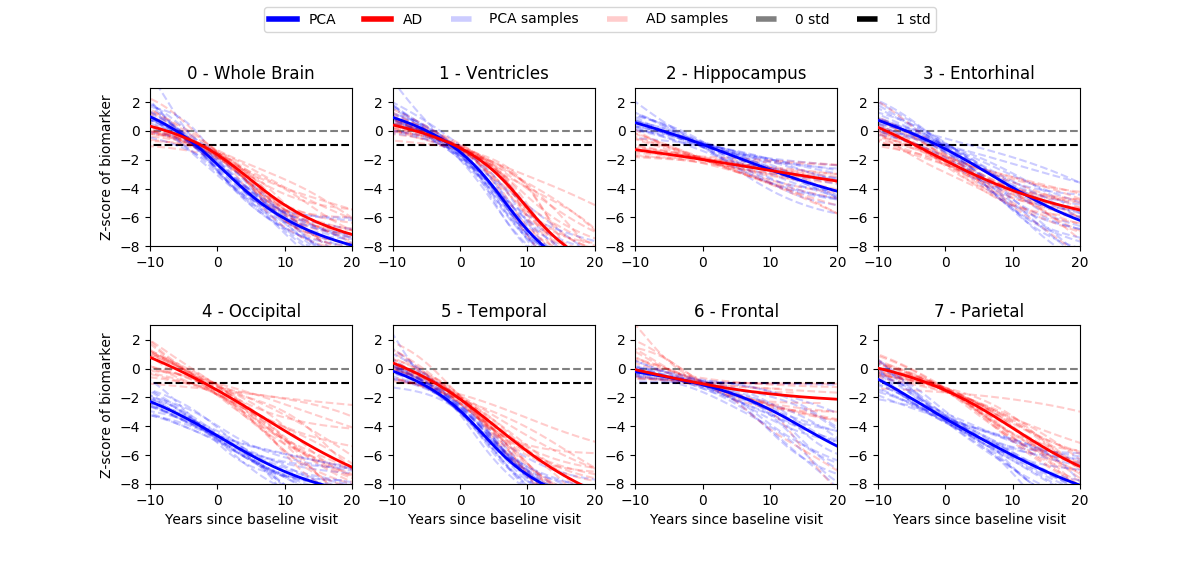
\includegraphics[scale=0.6,trim=100 0 100 0]{images/dem/mriSmallSebPaper_DEMStd_subplotsPcaAd.png}
 \caption{Mean trajectories of ROI volumes for PCA and tAD aligned on the same temporal scale along with samples from the posterior distribution showing the confidence in the mean trajectory. On the x-axis we show the number of years since baseline visit, while on the y-axis we show the z-score of the ROI volume relative to controls.}
 \label{trajDEMPcaAd}
\end{figure}

\section{Conclusion}
\label{sec:demConclusion}

% Summary
In this section we presented a longitudinal analysis of volume changes in PCA and tAD using the differential equation model. We compared the timing, rates and extent of atrophy across different regions in both PCA and tAD. Moreover, we also compared the evolution of each of these biomarkers across the two AD subtypes: tAD and PCA. While the patterns of tAD progression have been extensively studies using MRI biomarkers, there is significantly less literature on the progression of PCA. This analysis is the first to use data-driven disease progression models for studying atrophy evolution in PCA. Our analysis is also the first to directly compare MRI biomarkers in PCA vs tAD in terms of timing, rate and atrophy extent. 

% Limitations
There are several limitations with our analysis. First of all, we aligned the trajectories using the average biomarker value at patient baseline visit. This makes the assumption that the biomarker values corresponding to the stages of each patient at baseline only change linearly in that region. Secondly, the model fits each biomarker trajectory independently from the others and doesn't model biomarker correlations. Third, the confidence given by the posterior samples is not a true confidence interval, because these samples also have to be temporally aligned. This can bias the confidence interval, in making it smaller near the alignment point and larger at the ends. Moreover, the time $t=0$ is set as the time since baseline scan instead of disease onset. This becomes problematic when comparing across different diseases (PCA vs tAD) as symptoms might develop at different stages in the disease and this will influence when the subjects will come to the clinic for a baseline scan and assessment. 

% Future work drawing from the limitations
There are several possibilities for future work. The model can be extended to a multimodal framework by fitting an N-dimensional GP on the data and then integrating along all the biomarker values at the same time. This extension will remove the need to align the trajectories from different biomarker on the same temporal axis, but one still needs to set a $t=0$ starting point. Other clinical questions should also be explored, such as analysing subgroups within PCA, performing time to symptom onset analyses or asymmetry analyses. Other types of MRI biomarker measurements such as cortical thickness should also be analysed and linked to cognitive measures. 


\chapter{Voxelwise Temporal Clustering Model}
\label{chapter:voxelwise}

\section{Introduction}

% motivate the idea of avoiding a priori region specification
The main limitation of data-driven models such as the Event-Based Model (section \ref{sec:ebm}), the Differential Equation Model (section \ref{sec:dem}) or the Disease Progression Score (DPS) (section \ref{sec:dps}) is that they use a small set of biomarkers that are obtained by averaging MRI or PET measures across all voxels or vertices in a Region of Interest (ROI). This can be problematic, especially if different parts of the ROI, say the hippocampus, are affected at different speeds or timepoints in the disease process. Therefore, moving to a voxel-wise approach would allow one to estimate the fine-grained spatial distribution of atrophy, which would give new insights into the disease process and enable more precise staging. A voxel-wise disease progression model by Bilgel et al. \cite{bilgel2016multivariate} (see section \ref{sec:bilgel_voxelwise}) has been recently proposed to mitigate this problem, that uses amyloid measures in each voxel as its input data.

% highlight the limitations of bilgel et al. and explain the quantum leap
The voxel-wise model by \cite{bilgel2016multivariate} has two limitations: (1) it does not show which areas of the brain have a similar progression dynamics; (2) the biomarker trajectories are assumed to be linear, which are not suitable given that many biomarkers such as amyloid or tau plateau after a certain point. Moreover, the model uses a spatial correlation function for modelling correlation between voxels. While this is necessary, due to the nature of the imaging data, it has been shown that in different types of dementia atrophy patterns match functional networks, which are not spatially connected \cite{seeley2009neurodegenerative}. 

In this work, we present a new disease progression model with single vertex resolution that avoids assumptions on spatial correlation. We combine unsupervised learning and disease progression modelling to identify clusters of vertices on the cortical surface, with no spatial constraints, that show a similar trajectory of atrophy over a particular patient cohort. This formulation enables us to gain new insights into the spatial structure of atrophy in different diseases and also provides a novel parcellation of the brain based on temporal change. Moreover, each cluster of vertices has a corresponding sigmoidal trajectory, which avoids the limitation of linear trajectories in \cite{bilgel2016multivariate}. 

We first show using simulated data that our model is able to recover the underlying clusters, trajectory parameters and subject stages. We then apply our model to cortical thickness vertex-wise measures using ADNI and DRC datasets and highlight the new insights the model can give. Finally, we validate our model using cross-validation and by correlating the subject stages with cognitive measures.

% We first show that our algorithm gives similar answers on the two independent typical AD datasets (ADNI and local dataset). Secondly, when modelling distincts disease populations (PCA vs AD), our method finds different atrophy patterns which broadly reflect the known spatial distribution of atrophy in each condition. Finally, using cross calidation on the ADNI data we show that the model is robustly recovering the same clusters and that the stages are clinically meaningful, as they correlate with four different cognitive tests.

\section{Methods}
\label{sec:vwdpm_methods}

\subsection{Model}
\label{sec:vwdpm_model}

% progresison score, affine transformation
We seek to identify groups of image vertices that show a common trajectory during the disease course, while simultaneously placing each visit from each subject within that disease course. In a similar way to \cite{jedynak2012,donohue2014estimating,schiratti2015mixed}, we estimate a time shift and speed (or rate) of progression for each subject. We relate these time shifts and progression speeds by assigning each subject a disease stage which we will refer to as the Disease Progression Score (DPS). In contrast to \cite{jedynak2012,donohue2014estimating,schiratti2015mixed}, which model temporal trajectories for a small set of biomarker measures based on \emph{a priori} defined ROIs, we model temporal trajectories for each vertex on the cortical surface. Each trajectory is a function of the disease progression score (i.e. disease stage) of a subject. We estimate each subjects' time shift, progression speed and each trajectory from the data. The disease progression score $s_{ij}$ for subject $i$ at visit $j$ is defined as a linear transformation of age $t_{ij}$:

\begin{equation}
\label{eq:dps_vwdpm}
 s_{ij} = \alpha_i t_{ij} + \beta_i
\end{equation}
% sigmoidal functions
where $\alpha_i$ and $\beta_i$ represent the speed of progression and time shift (i.e. disease onset) of subject $i$. 

Our model assumes that the cortical thickness at each vertex on the cortical surface follows a sigmoidal trajectory $f(s)$ given the disease progression score $s$. We also assume that vertices are grouped into $K$ clusters and we model a unique trajectory for each cluster $k \in [1, \dots, K]$, which will be referred to as cluster trajectories. The sigmoidal function for cluster $k$ is parametrised as $\theta_k = [a_k,b_k,c_k,d_k]$ where 

\begin{equation}
\label{eq:dps_vwdpm2}
 f(s;\theta_k) = \frac{a_k}{1+exp(-b_k(s-c_k))} + d_k
\end{equation}

For a given subject $i$ at visit $j$, the value $V_l^{ij}$ of its cortical thickness at vertex $l$ is a random variable that has an associated discrete latent variable $Z_l \in [1, \dots, K]$ denoting the cluster it was generated from. The value of $V_l^{ij}$ given that it was generated from cluster $Z_l$ can be modelled as:

% TODO cannot use Z_l for the index of theta and for a random variable, use smth like Z_l = z_l, but watch out later on not to have conflicts.

% model for one voxel and label
\begin{equation}
\label{eq:dps_vwdpm3}
 p(V_l^{ij} | \alpha_i, \beta_i, \theta_{Z_l}, \sigma_{Z_l}, Z_l) = N(V_l^{ij} | f(\alpha_i t_{ij} + \beta_i | \theta_{Z_l}), \sigma_{Z_l})
\end{equation}
where $N(V_l^{ij} | f(\alpha_i t_{ij} + \beta_i | \theta_{Z_l}), \sigma_{Z_l})$ represents the pdf of the normal distribution that models the measurement noise along the sigmoidal trajectory of cluster $Z_l$, having variance $\sigma_{Z_l}$. Next, we assume the measurements from different subjects are independent, while the measurements from the same subject $i$ at different visits $j$ are linked using the disease progression score from equation \ref{eq:dps_vwdpm}, because we estimate only two parameters ($\alpha_i$ and $\beta_i$) using the data from all visits $j$. Moreover, we also assume a uniform prior on $Z_l$. This gives the following model:

% all subj are independent
\begin{equation}
\label{eq:dps_vwdpm4}
 p(V_l, Z_l | \alpha, \beta, \theta, \sigma) = \prod_{(i,j) \in I} N(V_l^{ij} | f(\alpha_i t_{ij} + \beta_i | \theta_{Z_l}), \sigma_{Z_l})
\end{equation}
where $I = {(i,j)}$ represents the set of all the subjects $i$ and their corresponding visits $j$. Furthermore, $V_l = [V_l^{ij} | (i,j) \in I]$ is the 1D array of all the values for vertex $l$ across every subject and corresponding visit. Vectors $\alpha = [\alpha_1, \dots, \alpha_S]$ and $\beta = [\beta_1, \dots, \beta_S]$, where $S$ is the number of subjects, denote the stacked parameters for the subject shifts. Vectors $\theta = [\theta_1, \dots, \theta_K]$ and $\sigma = [\sigma_1, \dots, \sigma_K]$, with $K$ being the number of clusters, represent the stacked parameters for the sigmoidal trajectories and measurement noise specific to each cluster.

We further assume all vertex measurements to be spatially independent, giving the complete data likelihood:

% all vertices are independent
\begin{equation}
\label{eq:dps_vwdpm5}
 p(V, Z | \alpha, \beta, \theta, \sigma) = \prod_l^L \prod_{(i,j) \in I} N(V_l^{ij} | f(\alpha_i t_{ij} + \beta_i | \theta_{Z_l}), \sigma_{Z_l})
\end{equation}
where $V = [V_1, \dots, V_L]$, $Z = [Z_1, \dots, Z_L]$, $L$ being the total number of vertices on the cortical surface. We recall that we don't want to enforce spatial correlation between vertices as we are interested to see if vertices from distinct areas of the brain are grouped together in the same cluster. Our assumption is also justified by the fact that we smoothed the cortical thickness images in the preprocessing steps. We get the final model log likelihood for incomplete data by marginalising over the latent variables $Z$:
\begin{equation}
\label{eq:dps_vwdpm6}
 p(V|\alpha, \beta, \theta, \sigma) = \prod_{l=1}^L \sum_{k=1}^K p(Z_l = k) \prod_{(i,j) \in I} N(V_l^{ij} | f(\alpha_i t_{ij} + \beta_i | \theta_k), \sigma_k)
\end{equation}
Therefore, the parameters that need to be estimated are $\Theta = [\alpha, \beta, \theta, \sigma]$ where $\alpha$ and $\beta$ are the subject specific shifting parameters while $\theta$ and $\sigma$ are the cluster specific trajectory and noise parameters. 

\subsection{Fitting the Model using EM}
\label{sec:vwdpm_fitting_model}

Due to the summing over the latent variables $Z$, it is not possible to find a closed form solution to the maximum likelihood. Therefore, we fit our model using Expectation-Maximisation, which is suitable given the large number of data points and parameters that need to be estimated. 

% We therefore seek to maximize:
% \begin{equation}
% \label{eq:EMgen}
% \argmax_{\Theta} E_{Z|V,\Theta^{old}} [log\ p(V,Z|\Theta)] + log\ p(\Theta) 
% \end{equation}
% where $\Theta^{old} = (\alpha^{old}, \beta^{old}, \theta^{old}, \sigma^{old})$ and $log\ p(\Theta)$ is a prior on the parameters.

\subsubsection{E-step}

In the Expectation step we seek to estimate which cluster has generated each of the $L$ vertices, given the current estimates of the cluster parameters $\theta_k^{old}, \sigma_k^{old}$ as well as the subject specific shift parameters $\alpha_i^{old}, \beta_i^{old}$. More formally, we seek to find $p(Z|V,\Theta^{old}) = \prod_l^L p(Z_l|V_l,\Theta^{old})$, given our independence assumption between vertices. Let us denote by $z_{lk} = p(Z_l = k | V_l,\Theta^{old})$. We then have:

\begin{equation}
 z_{lk} =  \frac{\prod_{(i,j) \in I} N(V_l^{ij} | f(\alpha_i^{old} t_{ij} + \beta_i^{old} | \theta_k^{old}), \sigma_k^{old})}{\sum_{m=1}^K \prod_{i,j \in I} N(V_l^{ij} | f(\alpha_i^{old} t_{ij} + \beta_i^{old} | \theta_m^{old}), \sigma_m^{old})}
\end{equation}
Ignoring the normalisation factor, we take the log and expand the pdfs of the normal distributions. This results in the following update equation for the E-step:

\begin{equation}
 log\ z_{lk} \propto  -\frac{1}{2} log\ (2 \pi \left(\sigma_k^{old}\right)^2) |I| - \frac{1}{2\left(\sigma_k^{old}\right)^2} \sum_{(i,j) \in I} (V_l^{ij} - f(\alpha_i^{old} t_{ij} + \beta_i^{old} | \theta_k^{old}))^2 
\end{equation}
The original probabilities can be easily recovered by exponentiating them and then normalising with respect to their sum.

\subsubsection{M-step}

In the Maximisation step we try to find $\Theta = (\alpha, \beta, \theta, \sigma)$ that maximise $E_{Z|V,\Theta^{old}} [log\ p(V,Z|\Theta)]$. Since there is no closed-form solution, we perform successive refinements of $\theta_k$ for each cluster $k$ and $\alpha_i, \beta_i$ for each subject $i$ until convergence. 

In order to get the update rule for the trajectory parameters $\theta_k$ corresponding to cluster $k$ we need to maximise the expected log likelihood with respect to $\theta_k$. We get the following simplified optimisation problem:

\begin{equation}
 \label{eq:theta}
 \theta_k = \argmin_{\theta_k} \left[\sum_{l=1}^L z_{lk} \sum_{(i,j) \in I} (V_l^{ij} - f(\alpha_i t_{ij} + \beta_i | \theta_k))^2 \right] - log\ p(\theta_k) 
\end{equation}
A similar equation is also obtained for $\sigma_k$. After estimating $\theta$ and $\sigma$ for every cluster, we use the new values to estimate the subject specific parameters $\alpha$ and $\beta$. Let $S$ be the number of subjects and $\alpha_i$, $\beta_i$ be the rate and shift for subject $i \in S$. We again maximise the expected log likelihood with respect to $\alpha_i$, $\beta_i$ independently, and after further simplifications we obtain the following problem:

\begin{equation}
\label{eq:alpha}
 \alpha_i, \beta_i = \argmin_{\alpha_i, \beta_i}  \left[ \sum_{l=1}^L \sum_{k=1}^K z_{lk} \frac{1}{2\sigma_k^2} \sum_{j \in I_i} (V_l^{ij} - f(\alpha_i t_{ij} + \beta_i | \theta_k))^2\right] - log\ p(\alpha_i, \beta_i)
\end{equation}

In summary, at every single M-step, we iterate between solving for $\theta$, $\sigma$ and solving for $\alpha$, $\beta$ using numerical optimisation until convergence. Due to the use of numerical optimisation, we are not guaranteed to find the global maxima for the expected log likelihood, but it has been shown that EM still works if we only find an increase in the log-likelihood \cite{bishop2006pattern}. This approach that involves a partial M-step is called Generalised EM.

\subsection{Initialisation and Implementation}
\label{sec:vwdpm_initialisation}
% initialisation
The optimisation algorithm is given in figure \ref{fig:algo_vwdpm}. Before starting the fitting process, we need to initialise $\alpha$, $\beta$ and the clustering probabilities $z_{lk}$. We set $\alpha_i$ and $\beta_i$ to be 1 and 0 respectively for each subject. We initialise $z_{lk}$ using k-means clustering using vectors $V_l$ having $|I|$ number of samples and $L$ features. Furthermore, as already explained in \cite{jedynak2012}, the scale of the DPS is arbitrary so we standardise the scores at each EM iteration such that the DPS of controls have a mean $\mu_N$ of zero and a standard deviation $\sigma_N$ of 1. This also requires a rescaling of the cluster parameters $\theta_k$.

In our implementation, we run the main EM loop until convergence of the clustering probabilities $z_{lk}$. At each M-step we also perform successive refinements of parameters $\theta$, $\alpha$ and $\beta$ using equations \ref{eq:theta}, \ref{eq:alpha} until convergence. For the numerical optimisation we used the Broyden-Fletcher-Goldfarb-Shanno (BFGS) algorithm that makes use of the first derivative of the objective function. In all datasets analysed, the method converges after maximum 25 EM iterations.\\

\begin{figure}
\begin{algorithm}[H]
%  \KwData{this text}
%  \KwResult{how to write algorithm with \LaTeX2e }
 Initialise $\alpha$, $\beta$, $z_{lk}$ \\
 \tcp*[l]{Outer loop}
%  $ a=1$\\ 
 \While{$z_{lk}$ not converged}{ 
  %M-step\\
   \tcp*[l]{M-step}
  \While{$\theta$, $\sigma$, $\alpha$, $\beta$ not converged}{
   \tcp*[l]{Optimise trajectories}
    \For{$k=1$ to $K$}{
      ${\theta_k = \argmin_{\theta_k} \sum_{l=1}^L z_{lk} \sum_{(i,j) \in I} (V_l^{ij} - f(\alpha_i t_{ij} + \beta_i | \theta_k))^2  - log\ p(\theta_k)}$\\
      ${\sigma_k^2 = \frac{1}{|I|} \sum_{l=1}^L z_{lk} \sum_{(i,j) \in I} (V_l^{ij} - f(\alpha_i t_{ij} + \beta_i | \theta_k))^2 - log\ p(\sigma_k)}$
    }
     \tcp*[l]{Optimise subject shifts}
    \For{$i=1$ to $S$}{
      ${\alpha_i, \beta_i = \argmin_{\alpha_i, \beta_i}  \left[ \sum_{l=1}^L \sum_{k=1}^K z_{lk} \frac{1}{2\sigma_k^2} \sum_{j \in I_i} (V_l^{ij} - f(\alpha_i t_{ij} + \beta_i | \theta_k))^2\right] - log\ p(\alpha_i, \beta_i)}$
    }
     \tcp*[l]{Re-scale subject shifts}
    \For{$i=1$ to $S$}{
      $\alpha_i = \frac{\alpha_i}{\sigma_N}, \beta_i = \frac{\beta_i - \mu_N}{\sigma_N}$
    }
     \tcp*[l]{Make trajectory parameters identifiable}
    \For{$k=1$ to $K$}{
      $\theta_k = \mbox{make\_identifiable}(\theta_k)$\\
      $\theta_k = \mbox{rescale}(\theta_k)$
    }
  }
  %E-step\\
   \tcp*[l]{E-step}
  \For{$l = 1$ to $L$}{
    \For{$k = 1$ to $K$}{
      ${ z_{lk} \propto  -\frac{1}{2} log\ (2 \pi \sigma_k^2) |I| - \frac{1}{2\sigma_k^2} \sum_{(i,j) \in I} (V_l^{ij} - f(\alpha_i t_{ij} + \beta_i | \theta_k))^2  }$
    }
  }
 }
\end{algorithm}
\caption{The model fitting algorithm.}
\label{fig:algo_vwdpm}
\end{figure}

\section{Simulation results}
\label{sec:vwdpm_simulations}

% method
We first tested the model in a toy scenario using synthetic data to see how well the cluster probabilities, trajectories and subject shifts are recovered. We generated our data as follows:
\begin{enumerate}
 \item sampled age and shift parameters from 300 subjects with 4 timepoints (each timepoint 1 year apart), with $t_{i1} \sim U(40,80)$, $\alpha_i \sim N(1, 0.05)$, $\beta_i \sim N(0, 10)$
 \item generated three sigmoids with different center points and slopes (Fig. \ref{fig:synThetaRes}, red lines). 
 \item generated a random cluster assignment for $L = 1,000$ vertices, i.e. every vertex $l$ was assigned to a cluster $a[l] \in \{1,2,3\}$
 \item sampled a set of $L$ perturbed trajectories $\theta_l$ from each of the original trajectories, one for each vertex (Fig. \ref{fig:synThetaRes}, gray lines)
 \item sampled subject data for every vertex $l$ from its corresponding perturbed trajectory $\theta_l$ with $\sigma_l = 0.5$
\end{enumerate}
To fit the data we used a uniform prior on the parameters $\theta$ and $\sigma$ and an informative prior on $\alpha$ and $\beta$, with $p(\alpha_i) \sim \Gamma(49,70)$ and $\beta_i \sim N(0,1)$. We also normalised age to have a mean of 0 and standard deviation of 1 and rescaled the DPS and cluster trajectories accordingly. After convergence, we calculated the agreement between the final clustering probabilities and the true clustering assignments as $A = \frac{1}{L}\sum_{l=1}^L p(Z_l = a[l])$. However, the recovered clusters can be found in a permuted order, so we used the permutation that yielded the highest agreement $A$. The method also requires us to set the number of clusters \emph{a priori}, so in order to find the optimal number of clusters we used model selection with the Bayesian Information Criterion (BIC). 

% Results
The BIC analysis correctly predicted 3 clusters for this synthetic experiment. Using three clusters, we also obtained a clustering agreement of $A = 1.0$. Figure \ref{fig:synThetaRes} shows the original trajectories and the recovered trajectories using our model, plotted against the disease progression score on the x-axis and the vertex value on the y-axis. Moreover, in Fig. \ref{fig:synShiftRes} we plotted the recovered DPS of each subject along with the true DPS. 

% Conclusion
The results show that the model accurately estimated which clusters generated each vertex. Moreover, the recovered trajectories are close to the true trajectories, with some errors for the trajectories corresponding to clusters 1 and 2. The recovered DPS also shows good agreement with the true DPS, with the exception of a few subjects with DPS greater than 2.5. This is explained by the fact that there is not enough signal in that DPS range in terms of trajectory dynamics (i.e. trajectories are mostly flat). The simulation confirms that our model is able to recover the hidden clusters, trajectory parameters and the subject specific parameters. However, more realistic simulations with varying noise levels and numbers of clusters are required to understand the limitations of the model and find out when it fails to recover the true parameters. 


\begin{figure}
\begin{subfigure}[b]{0.75\textwidth}
  \hspace{-2em}
  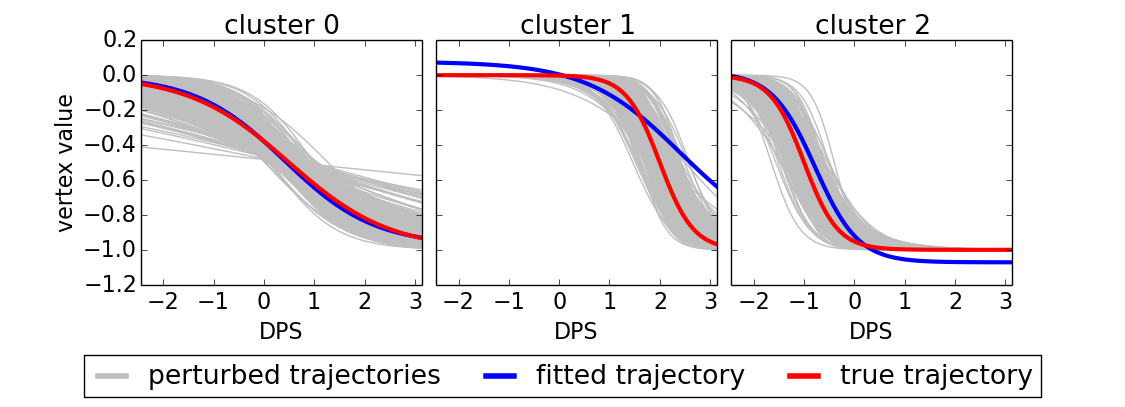
\includegraphics[width=1.15\textwidth]{images/vwdpm//synThetaRes_gensigInitk-meansCl3Pr1Ra0_VWDPMStd.png}
  \caption{}
  \label{fig:synThetaRes}
\end{subfigure}
\hspace{-1em}
\begin{subfigure}[b]{0.24\textwidth}
\centering
  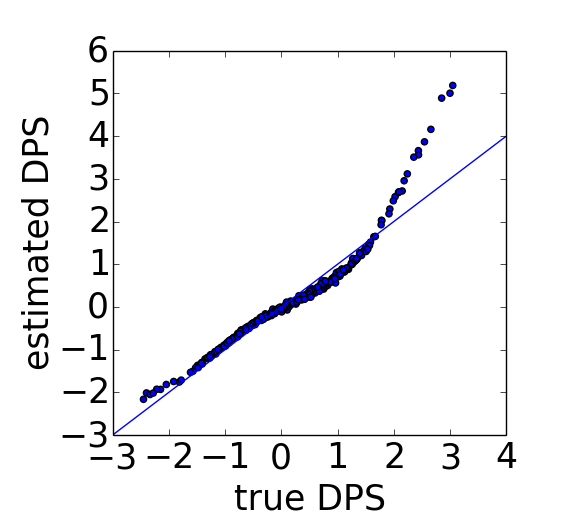
\includegraphics[width=1.2\textwidth]{images/vwdpm/synShiftsRes_gensigInitk-meansCl3Pr1Ra0_VWDPMStd.png}
    \vspace{0.7em}
  \caption{}
  \label{fig:synShiftRes}
\end{subfigure}
\caption{(a) Reconstructed temporal trajectories (blue) from the synthetic data along with the true trajectories (red). The data was generated from the perturbed trajectories, which in turn were generated from the true trajectories. (b) Estimated subject-specific disease progression scores compared to the true scores.}
\end{figure}

\section{Experimental results}
\label{sec:vwdpm_results}

\subsection{Data acquisition and preprocessing}

We analysed cortical thickness measures from two datasets: ADNI and DRC dataset. For ADNI, we downloaded from http://adni.loni.usc.edu/ all T1 MRI images that have undergone gradwarping, intensity correction and scaling for gradient drift. We included subjects that had at least 4 scans, in order to ensure we get a robust estimate of the subject specific parameters. This resulted in 328 subjects with an average number of 4.95 scans each. The DRC dataset consisted of T1 MRI scans from 31 healthy controls, 32 PCA and 23 typical typical AD subjects with at least 3 scans each and an average of 5.26 scans per subject.

% freesurfer pipeline
On both datasets, in order to extract reliable thickness measures we ran the Freesurfer longitudinal pipeline \cite{reuter2012within}, which first registers the MRI images to an unbiased within-subject template space using inverse-consistent registration. The longitudinally registered images were then registered to the Freesurfer template and smoothed at various full-width/half-max (FWHM) values. We used the FWHM zero level and for each vertex we averaged the thickness levels from both hemispheres. Finally, we standardised the data from each vertex with respect to the values of that vertex in the control population.  Each of the final images had a resolution of 163,842 vertices on the cortical surface. 


\subsection{Results with ADNI and DRC datasets}
\label{sec:vwdpm_results_sub}

% Motivation: 
% 1. see how the patterns of atrophy look in the two diseases tAD and PCA look like. 
% 2. see if similar results are obtained on two independent datasets
% 3. see if different atrophy patterns are obtained in tAD vs PCA, and if they match previous studies.
Using ADNI and DRC datasets, we were interested to find out the spatial distribution of cortical atrophy, as well as the rate and timing of this atrophy process. In particular, we would like to find out: (1) if we get similar results using our model on two independent tAD datasets: ADNI and DRC datasets and (2) if we get different patterns of atrophy on distinct diseases (tAD and PCA) that match previous studies. 

% Results
BIC analysis predicted that the optimal number of clusters is two for the ADNI cohort and three for both tAD and PCA subjects from the DRC cohort. In order to make the results easily comparable across the different datasets, we ran all experiments using 3 clusters. Fig. \ref{fig:adniClust} shows the results of our model using all ADNI subjects, where we coloured points on the cortical surface according to the cluster they most likely belong to. We assigned a colour to each cluster according to the slope of its corresponding trajectory, ranging from red (high slope suggesting a fast rate of atrophy) to blue (low slope suggesting a slow rate of atrophy). In Fig. \ref{fig:adniTraj} we also show the resulting cluster trajectories with samples from the posterior distribution of each $\theta_k$. We repeated the same analysis on the DRC cohort, separately for the tAD subjects (Fig. \ref{fig:drcClustAD} and \ref{fig:drcTrajAD}) and PCA subjects (Fig. \ref{fig:drcClustPCA} and \ref{fig:drcTrajPCA}). 

% Conclusions - first talk about tAD then about PCA
We notice that in tAD subjects using both ADNI and the DRC dataset (Fig. \ref{fig:clustTrajAll}), there is widespread atrophy in most temporal, parietal and frontal areas (red cluster), with the notable exception of the motor cortex and the occipital lobe. These patterns of atrophy are similar across the two different datasets. Moreover, the spatial distribution of cortical thinning found with our technique resembles results from previous longitudinal studies \cite{dickerson2009cortical,thompson2001cortical}. However, in contrast to those approaches, our model gives insight into the timing, rate and extent of atrophy.

In the PCA subjects (Fig. \ref{fig:drcClustPCA}), we find that the atrophy is more focused on the posterior part of the brain, mostly the posterior parietal and occipital, with more limited spread in the superior temporal and inferior frontal. This is in contrast with the tAD patterns in the other datasets, that lacks the focus on posterior parietal and occipital regions. This posterior pattern of atrophy also matches previous findings in the literature \cite{crutch2012posterior}. For all datasets, we find that the cluster trajectories differ less in timing and more in the slope and minima/maxima values at which they plateau (Fig. \ref{fig:adniTraj}, \ref{fig:drcTrajAD}, \ref{fig:drcTrajPCA}). Our model therefore predicts that regions on the cortical surface are all affected roughly at the same time, but the rate and extent to which they are affected is different.   

\newcommand{\scalingFactor}{1}

\newcommand{\gradLimLeft}{-1.6}
\newcommand{\gradLimRight}{1.6}

% \newcommand{\scalingFactorLeftFig}{1.2}
\newcommand{\scalingFactorBrains}{1}
\newcommand{\scalingFactorTraj}{1.1}

% FWHM0 avg thickness map MCI & AD
\begin{figure}[h]
  \centering

  % do the legend colorbar
  \begin{subfigure}[b]{\textwidth}
   \centering
  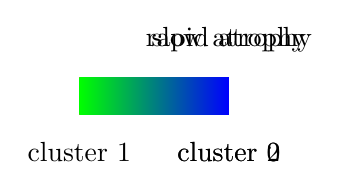
\begin{tikzpicture}[scale=1.9]
    \shade[left color=red,right color=green] (\gradLimLeft,2.5) rectangle (0,2.75);
    \shade[left color=green,right color=blue] (0,2.5) rectangle (\gradLimRight,2.75);
    \node[inner sep=0] (corr_text) at (\gradLimLeft,2.25) {cluster 0};
    \node[inner sep=0] (corr_text) at (0,2.25) {cluster 1};
    \node[inner sep=0] (corr_text) at (\gradLimRight,2.25) {cluster 2};
    \node[inner sep=0] (corr_text) at (\gradLimLeft,3) {rapid atrophy};
    \node[inner sep=0] (corr_text) at (\gradLimRight,3) {slow atrophy};
  \end{tikzpicture}
%     \caption{}
%       \label{fig:adniClust}
  \vspace{1em}
  \end{subfigure}
  
  %%%%%%%%%%%%%%%%%%% BRAINS %%%%%%%%%%%%%%5%%%%%%
  
  \begin{subfigure}[b]{0.3\textwidth}
   \centering
  \begin{tikzpicture}[scale=\scalingFactor, every node/.style={scale=\scalingFactor}]
    \node[inner sep=0] (image) at (0,0) {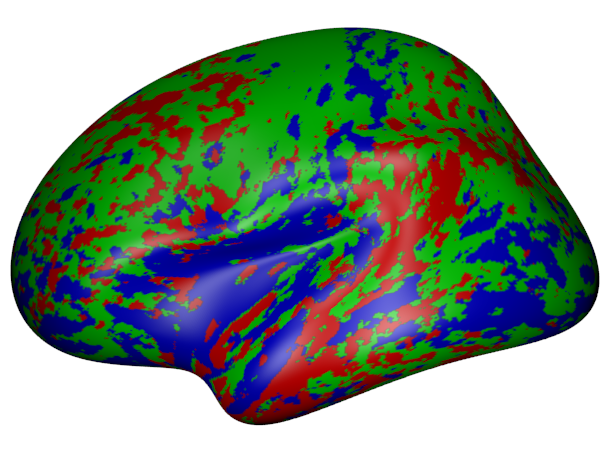
\includegraphics[width=\scalingFactorBrains\textwidth]{images/vwdpm/blend14_adniThavgFWHM0InithistCl3Pr0Ra1_VWDPMStd.png}}; 
    \node[inner sep=0] (label) at (0,3.5) {tAD - ADNI};
  \end{tikzpicture}
    \caption{}
      \label{fig:adniClust}
  \end{subfigure}
   \begin{subfigure}[b]{0.3\textwidth}
  \centering
  \begin{tikzpicture}[scale=\scalingFactor]
    \node[inner sep=0] (corr_text) at (0,0) {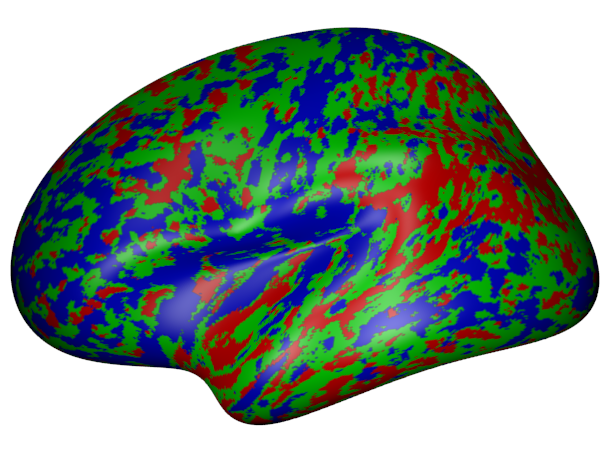
\includegraphics[width=\scalingFactorBrains\textwidth]{images/vwdpm/drcThavgFWHM0InithistCl3Pr0Ra1_VWDPMStdAD_blend24.png}};
    \node[inner sep=0] (label) at (0,3.5) {tAD - DRC dataset};
  \end{tikzpicture}
    \caption{}
      \label{fig:drcClustAD}
  \end{subfigure}
   \begin{subfigure}[b]{0.3\textwidth}
  \centering
  \begin{tikzpicture}[scale=\scalingFactor, every node/.style={scale=\scalingFactor}]
    \node[inner sep=0] (corr_text) at (0,0) {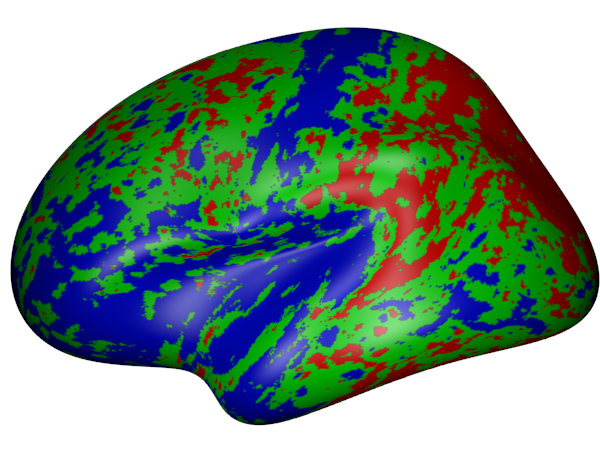
\includegraphics[width=\scalingFactorBrains\textwidth]{images/vwdpm/drcThavgFWHM0InithistCl3Pr0Ra1_VWDPMStdPCA_blend24.png}};
    \node[inner sep=0] (label) at (0,3.5) {PCA - DRC dataset};
  \end{tikzpicture}
    \caption{}
      \label{fig:drcClustPCA}
  \end{subfigure}
  
  %%%%%%%%%%%%%%%%%%%%%% trajectories %%%%%%%%%%%%%%%%%%%%%%%
  
    \begin{subfigure}[b]{0.3\textwidth}
    \centering
%     \vspace{-2em}
    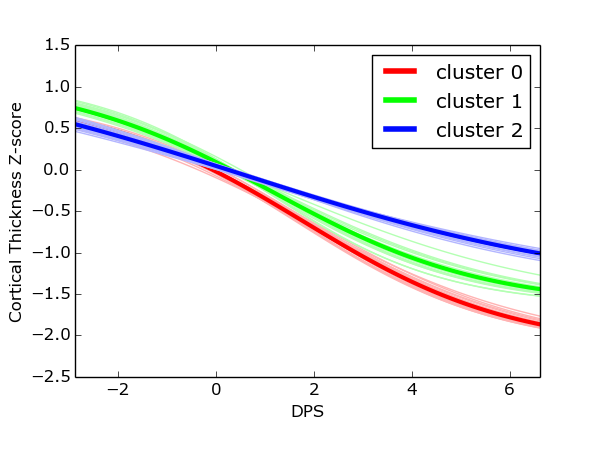
\includegraphics[width=\scalingFactorTraj\textwidth]{images/vwdpm/trajSamplesOneFig_adniThavgFWHM0InithistCl3Pr0Ra1_VWDPMStd.png}
    \caption{}
      \label{fig:adniTraj}
  \end{subfigure}
      \begin{subfigure}[b]{0.3\textwidth}
    \centering
%     \vspace{-2em}
    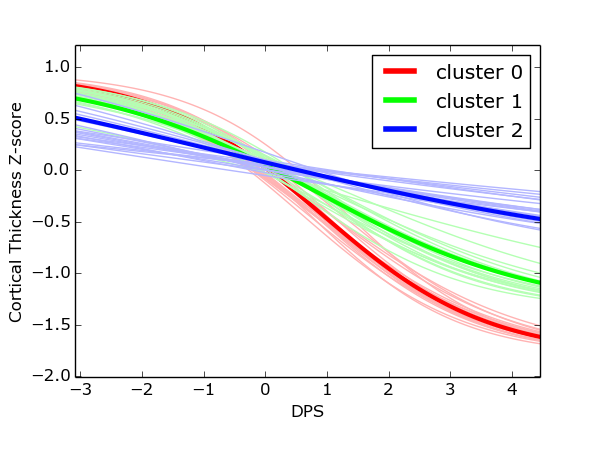
\includegraphics[width=\scalingFactorTraj\textwidth]{images/vwdpm/trajSamplesOneFig_drcThavgFWHM0InithistCl3Pr0Ra1_VWDPMStdAD.png}
    \caption{}
      \label{fig:drcTrajAD}
  \end{subfigure}
    \begin{subfigure}[b]{0.3\textwidth}
    \centering
%     \vspace{-2em}
    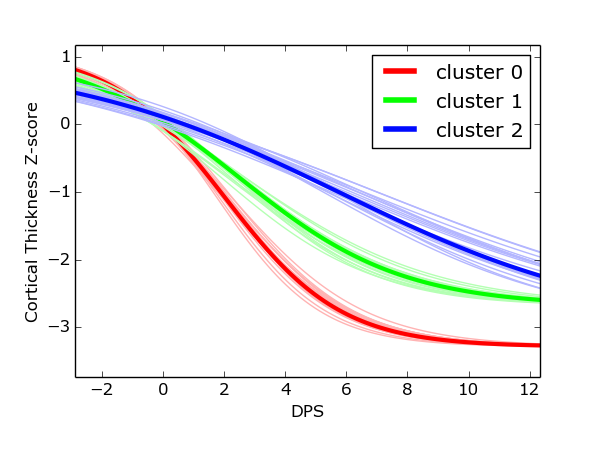
\includegraphics[width=\scalingFactorTraj\textwidth]{images/vwdpm/trajSamplesOneFig_drcThavgFWHM0InithistCl3Pr0Ra1_VWDPMStdPCA.png}
    \caption{}
      \label{fig:drcTrajPCA}
  \end{subfigure}
  
  \caption{(a) Clustering results on the ADNI data using our model, where each cluster is coloured according to the slope of its corresponding trajectory, from red (high slope suggesting very affected areas) to blue (low slope suggesting less affected areas). (d) The corresponding trajectories and samples from the posterior distribution of the trajectory  parameters for the three clusters in ADNI. The same analysis is shown also for (b, e) tAD subjects from the DRC cohort and (c, f) PCA subjects from the DRC cohort.}
  \label{fig:clustTrajAll}

\end{figure}

\subsection{Model Validation}
\label{sec:vwdpm_validation}

% motivation, i.e. what we wanted to test
We tested robustness of the model by performing 10-fold cross validation (CV) on ADNI. Our motivation was to test the following: (1) if similar spatial clustering is estimated at each fold, as quantified by Dice score overlap (2) if the stages of the test subjects were consistent (i.e. were increasing for follow-up visits) and (3) if the stages of test subjects are clinically meaningful, by correlating them with cognitive tests such as Clinical Dementia Rating Scale - Sum of Boxes (CDRSOB), Alzheimer's Disease Assessment Scale - Cognitive (ADAS-COG), Mini-Mental State Examination (MMSE) and Rey Auditory and Verbal Learning Test (RAVLT).

% results 
Fig \ref{fig:ADNICVbrains} shows the clusters that were estimated at each fold from the training data only. Moreover, in Fig. \ref{fig:stagingConsist} we plot the estimated DPS (i.e. disease stage) of each subject from the test set against their age.

% conclusion
The results in Fig. \ref{fig:ADNICVbrains} prove that the model is robust in cross-validation, as the estimated clusters are all very similar across folds. The average Dice scores we obtained across all pairs of folds were 0.89, 0.89 and 0.90 for clusters 0, 1 and 2 respectively. Furthermore, 84\% of the subjects analysed show increased stages across their follow-up visits, proving that the estimated stages are mostly consistent. Finally, the stages of test subject correlate with clinical measures such as CDRSOB ($\rho = 0.41$, $p < 1e-66$), ADAS-COG ($\rho = 0.40$, $p < 1e-62$), MMSE ($\rho = 0.39$, $p < 1e-58$) and RAVLT ($\rho = 0.35$, $p < 1e-46$), demonstrating that the stages have clinical validity.

\newcommand{\outFoldADNICVbrains}{images/vwdpm/crossvalid/adniThavgFWHM0Initk-meansCl3Pr0Ra1_VWDPMMean}

\begin{figure}[h]
    \centering
    
    \begin{subfigure}[b]{0.19\textwidth}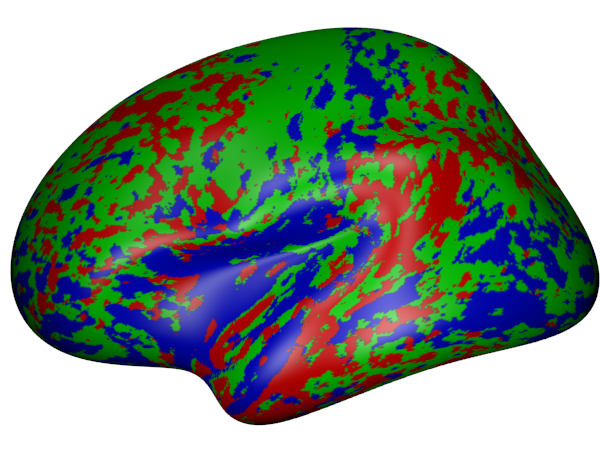
\includegraphics[width=\textwidth]{\outFoldADNICVbrains/blend0.png}\end{subfigure}
    \begin{subfigure}[b]{0.19\textwidth}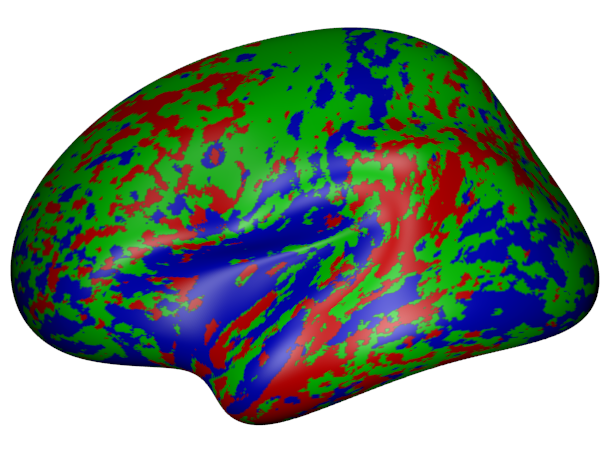
\includegraphics[width=\textwidth]{\outFoldADNICVbrains/blend1.png}\end{subfigure}
    \begin{subfigure}[b]{0.19\textwidth}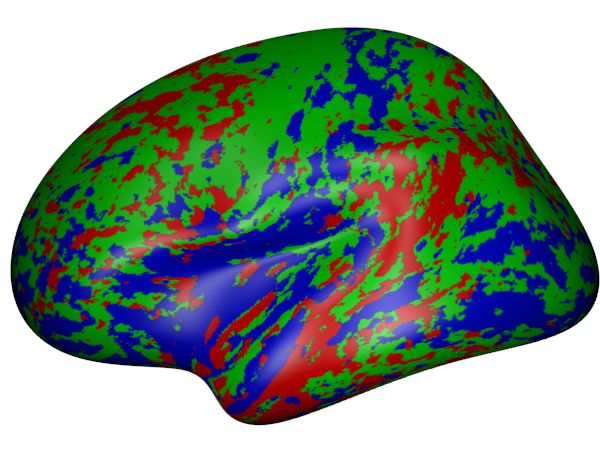
\includegraphics[width=\textwidth]{\outFoldADNICVbrains/blend2.png}\end{subfigure}
    \begin{subfigure}[b]{0.19\textwidth}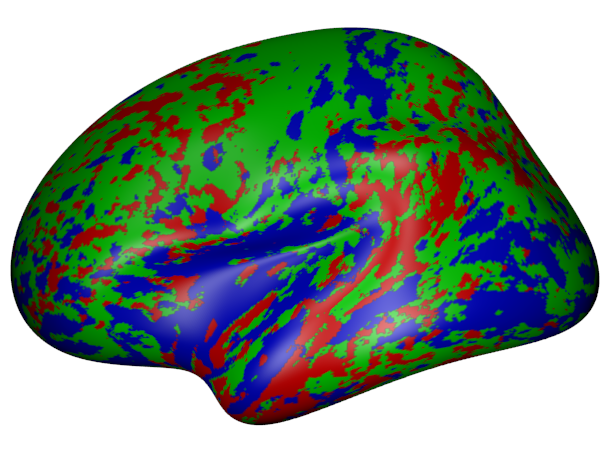
\includegraphics[width=\textwidth]{\outFoldADNICVbrains/blend3.png}\end{subfigure}
    \begin{subfigure}[b]{0.19\textwidth}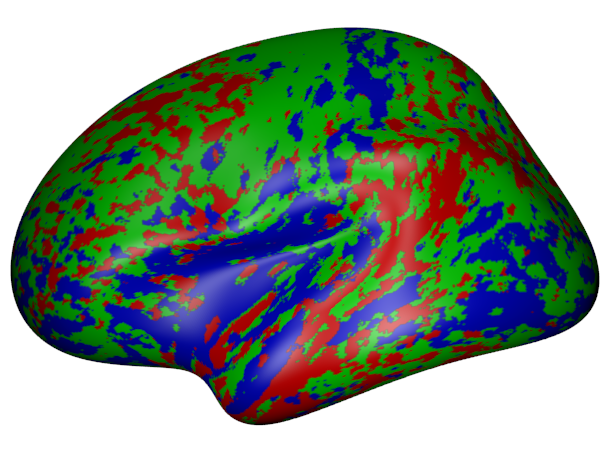
\includegraphics[width=\textwidth]{\outFoldADNICVbrains/blend4.png}\end{subfigure}
    \begin{subfigure}[b]{0.19\textwidth}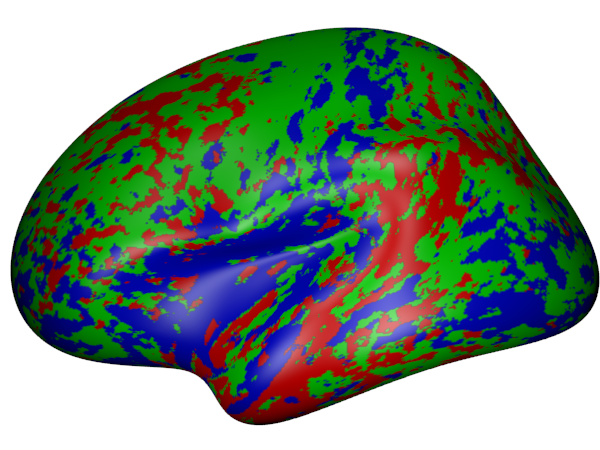
\includegraphics[width=\textwidth]{\outFoldADNICVbrains/blend5.png}\end{subfigure}
    \begin{subfigure}[b]{0.19\textwidth}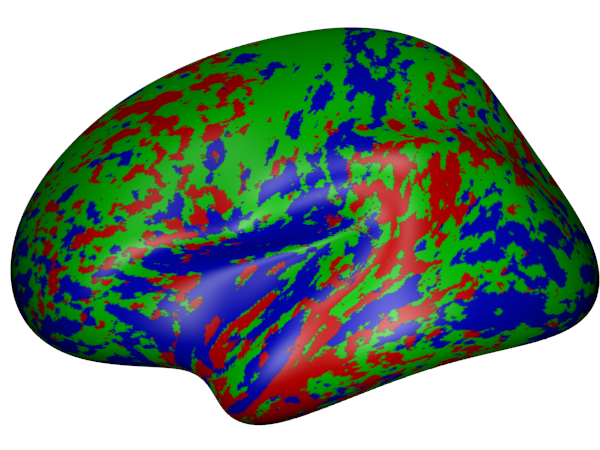
\includegraphics[width=\textwidth]{\outFoldADNICVbrains/blend6.png}\end{subfigure}
    \begin{subfigure}[b]{0.19\textwidth}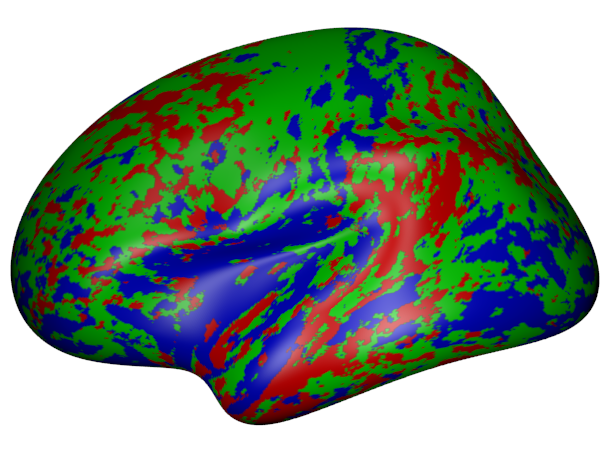
\includegraphics[width=\textwidth]{\outFoldADNICVbrains/blend7.png}\end{subfigure}
    \begin{subfigure}[b]{0.19\textwidth}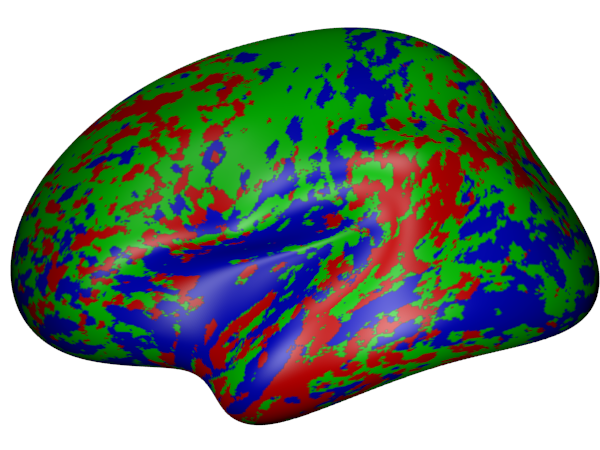
\includegraphics[width=\textwidth]{\outFoldADNICVbrains/blend8.png}\end{subfigure}
    \begin{subfigure}[b]{0.19\textwidth}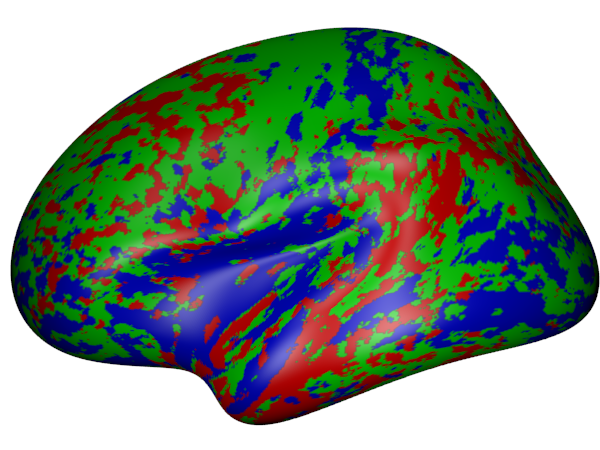
\includegraphics[width=\textwidth]{\outFoldADNICVbrains/blend9.png}\end{subfigure}
    
    \caption{Clusters estimated for each of the 10 cross-validation folds in ADNI. As before, each cluster is coloured according to the slope of its corresponding trajectory, from red (high rate of atrophy) to blue (low rate of atrophy).}
    \label{fig:ADNICVbrains}
\end{figure}


\begin{figure}[h]
    \centering
    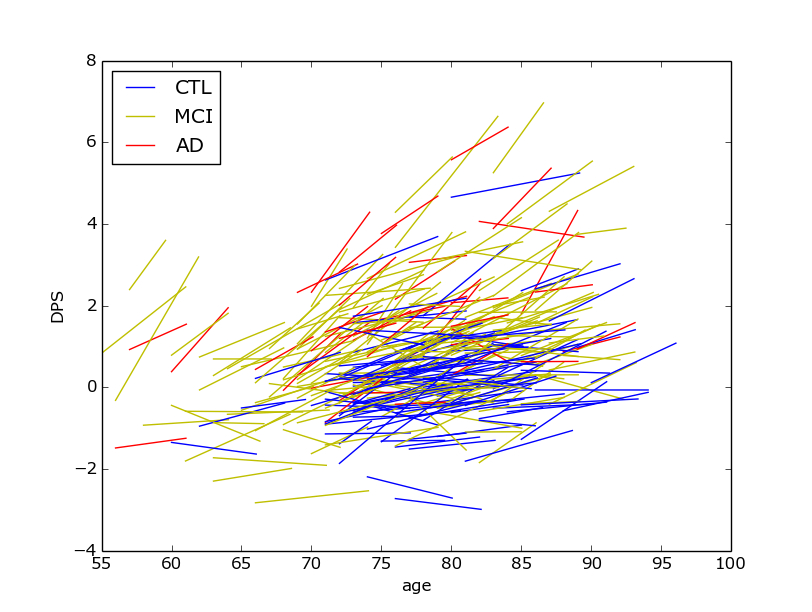
\includegraphics[width=0.5\textwidth]{images/vwdpm/crossvalid/stagingConsist_adniThavgFWHM0Initk-meansCl3Pr0Ra1_VWDPMMean.png}
    \caption{The disease progression score for each subject from the ADNI dataset estimated during 10-fold cross validation. Each line represents an individual $i$ with different visits $j$. Later visits generally have a higher corresponding stage.}
    \label{fig:stagingConsist}
\end{figure}

\section{Discussion}
\label{sec:vwdpm_discussion}

% summary -> other types of data -> not regress against age -> disease progression space -> model worked ok -> stages better than with static ROIs
We presented a model of disease progression that clusters vertex-wise measures of cortical thickness based on similar temporal dynamics. The model highlights, for the first time, groups of cortical vertices that exhibit a similar temporal trajectory over the population. This provides a new way to parcellate the brain that is specific to the temporal trajectory of a particular disease. The model also finds the optimal temporal shift and progression speed for every subject. We have applied it to cortical thickness vertex-wise data from ADNI and DRC cohorts. Our model found similar patterns of atrophy dynamics in the tAD subjects using two independent datasets. Moreover, it also found different patterns of atrophy dynamics on two distinct diseases: typical AD and PCA. 

% Limitations of the model
% a priori # of clust -> but can do BIC maximisation -> traj assumed sigmoidal -> but can use non-parametric curves -> Bias due to z-score normalisation - > susceptible to registration errors
The model has some limitations. First of all, we have assumed that cluster trajectories follow sigmoidal shapes, which might not be the case for many types of biomarkers such as cortical thickness. Another limitation of the model is that it assumes all subjects follow the same disease progression pattern, which might not be the case in heterogeneous datasets such as ADNI or the DRC cohort. Furthermore, the data we analysed has been standardised with respect to controls, which can introduce biases due to the fact that controls might already show some abnormalities in cortical thickness.

% future work on technical improvements, motivated by the limitations mentioned before
There are several potential avenues of future research. While we have only used the model for studying cortical thickness, one can also apply it to other types of data such as amyloid images or Jacobian compression maps. On the methodological side, the assumption of sigmoidal trajectories can be avoided using non-parametric curves such as Gaussian Processes or self-modelling regression techniques \cite{donohue2014estimating}. One could also model different progression dynamics for distinct groups in the population by clustering subjects together like the approach of \cite{young2015multiple}. The analysis could also be improved by using only amyloid negative controls for data standardisation.

% potential impact, clinical applications, work required to get there
Our approach can be used for accurately predicting and staging neurodegenerative disease progression. This is promising for patient prognosis, as well as in clinical-trials for assessing efficacy of a putative treatment for slowing down the degeneration process.

\chapter{Project Plan}
\label{chapter:plan}

In this section we present our future work plan until the end of the PhD. In section \ref{sec:plan_vox} we suggest further modelling that can be done using the voxelwise temporal clustering model presented in chapter \ref{chapter:voxelwise}. In section \ref{sec:plan_perf_eval} we present further analysis that should be done on performance evaluation of disease progression models \ref{sec:plan_perf_eval}. In section \ref{sec:plan_pca_paper_seb} we present further applications for our disease progression models, more precisely on the PCA vs tAD comparison. Finally, in Fig. \ref{fig:plan_gantt} we present a Gantt chart showing the proposed work plan.

\section{Voxelwise Temporal Clustering Model}
\label{sec:plan_vox}

We plan to extend the work done on the voxelwise temporal clustering in several ways and do further analysis. These are summarised in the list below:
\begin{enumerate}
 \item Must do:
 \begin{enumerate}
  \item Run model on amyloid PET imaging from ADNI. This would complement the work currently done using cortical thickness and demonstrate the different types of data which can be analysed by the model. 
  \item Perform more validation on ADNI and DRC datasets. This can include: correlation of stages with cognitive measures, more staging consistency metrics and other goodness of fit measures.
  \item Test a similar model that fits trajectories according to the mean value of vertex measurements in every cluster. We believe that this model gives very similar results but it can run much faster, as the sum over every vertex in equation \ref{eq:dps_vwdpm6} will disappear. 
 \end{enumerate}
 \item Should do:
 \begin{enumerate}
  \item Extensive testing on synthetic data. This can include experiments for many different types of trajectories and number of clusters. For each experiment we plan to plot error-bars showing the error on subject staging and recovered trajectory parameters.
 \end{enumerate}
 \item Might do:
 \begin{enumerate}
  \item Extend model to non-parametric curves such as Gaussian Processes (if time permits). This would involve changing the fundamentals of the model and can be difficult to fine-tune the parameters for the model on each dataset, otherwise the model can easily overfit. 
  \item Extend the model to analyse multimodal data. In order to construct an accurate temporal axis of the disease progression, it can additionally use cognitive tests, CSF biomarkers or combine different voxelwise imaging modalities (cortical thickness + amyloid images). Combining multiple biomarkers is important, as they become abnormal at different stages of the disease. 
  \item Explore other types of voxel dependence, such as spatial correlation functions. 
  \item Extend the model to account fit subgroups of subjects with different clusters of voxels. This will account for disease heterogeneity.
 \end{enumerate}
\end{enumerate}


\section{Performance Evaluation}
\label{sec:plan_perf_eval}

We plan to extend the work on performance evaluation in order to turn this into a comprehensive evaluation of many different metrics (section \ref{sec:plan_metrics}) and disease progression models (section \ref{sec:plan_models}). Based on this work, we also consider getting involved in a prediction challenge using the ADNI dataset. This challenge will involve training some models on current ADNI data and using a subsequent release of ADNI data as the testing set. 

\subsection{Metrics}
\label{sec:plan_metrics}

We plan to further evaluate the following performance metrics or scenarios:
\begin{enumerate}
 \item Must do:
 \begin{enumerate}
 \item Correlation of stages with cognitive measures
 \item Goodness of fit: AIC, BIC
 \item Synthetic data - error in estimating the true parameters
 \end{enumerate}
 \item Should do:
 \begin{enumerate}
 \item Resampling methods: cross-validation, bootstrapping (measure std of estimated parameters)
 \item Robustness to added noise levels in real data
 \end{enumerate}
 \item Might do:
 \begin{enumerate}
  \item Experiment design metrics: these will test which biomarkers are the most informative. This can help make the clinical studies more economical by removing scans or cognitive tests that do not bring in new information.
 \end{enumerate}
\end{enumerate}

\subsection{Models}
\label{sec:plan_models}

We plan to incorporate other fundamentally different models such as:
\begin{enumerate}
 \item Must do:
 \begin{enumerate}
 \item Disease Progression Score (DPS) (Jedynak et al. \cite{jedynak2012computational})
 \item Self-Modelling Regression (SEMOR) (Donohue et al. \cite{donohue2014estimating})
 \end{enumerate}
 \item Might do:
 \begin{enumerate}
 \item Riemannian manifold model (Schiratti et al. \cite{schiratti2015learning})
 \end{enumerate}
Testing other models such as these will help us understand if the assumptions they make are reasonable for the ADNI biomarkers. Moreover, based on the results we will also be able to point out improvements in these models. 
 
 
\end{enumerate}


\subsection{Dataset}
\label{sec:plan_dataset}

Our plan is to do the performance analysis only on the ADNI dataset. We will carefully choose a set of biomarkers derived from MRI (ROI volumes, cortical thickness, atrophy rates), CSF (amyloid-beta, tau), PET (FDG, PIB) and cognitive tests. We need to be careful so that the choice of these biomarkers will not favour certain models. 

\section{PCA vs tAD Analysis}
\label{sec:plan_pca_paper_seb}

We plan to continue the application of our disease progression models to PCA and tAD analysis on the DRC dataset. We suggest to perform the following analysis\footnote{ideas proposed by Dr. Sebastian Crutch}:

\begin{enumerate}
 \item Must do:
\begin{enumerate}
 \item Study rates of atrophy for different PCA subtypes. This analysis will be similar to the one in section \ref{ebm:pca_subgroups}, but will study atrophy rates instead of timing. This can be done with a simple linear mixed effects model or, if there is enough data, with the differential equation model. We would like to test the following hypotheses:
 \begin{enumerate}
  \item Vision subgroup: greater occipital lobe atrophy compared to other subgroups?
  \item Space subgroup: greater superior parietal atrophy compared to other subgroups?
  \item Object subgroup: greater inferior temporal atrophy compared to other subgroups?
 \end{enumerate}
 \item Study the continuum of the three subgroups: build EBM with each subgroup separately, and then try to assign subjects to different models. Plot the normalised likelihoods of belonging to each model on a triangle. 
\end{enumerate}
 \item Should do:
 \begin{enumerate}
 \item Predict progression of cognitive tests from imaging biomarkers at baseline. This task would comprise generating cross-sectional occipital-hippocampal volume discrepancy values at baseline and then test whether different subgroups on this occipital-hippocampal continuum predict different longitudinal patterns of cognitive impairment. More precisely, we hypothesise that patients that have a lower occipital volume at baseline (PCA-like) will have early visual loss with memory spared until later. On the other hand, patients who have a lower hippocampal volume at baseline (tAD-like) will have earlier multi-domain cognitive impairment. 
 \end{enumerate}
 \item Might do:
 \begin{enumerate}
  \item Repeat the same analysis as in 1 (a) but for cortical thickness measures. 
  \item Study the relationship between posterior and anterior grey matter loss. 
  \begin{enumerate}
   \item Based on anatomical subgroups, test if greater inferior posterior atrophy predict greater inferior anterior atrophy and vice versa.
   \item Test if dorsolateral prefrontal lobe atrophy and cortical thinning differ significantly between the three clinical subgroups as follows: (Highest atrophy) Space $>$ Object $>$ Vision (Lowest atrophy). 
   \item Test if inferior prefrontal atrophy and cortical thinning differ significantly between the three subgroups as follows: (Highest atrophy) Object $>$ Space $>$ Vision (Lowest atrophy). 
  \end{enumerate}
  \item Asymmetry analyses: 
  \begin{enumerate}
   \item Measure timing of atrophy: Run the EBM on PCA and tAD using separate biomarkers for left and right hemisphere regions.
   \item Measure rate and extent of atrophy: Run the DEM as above. In addition to that, also plot each left vs right ROI trajectories and measure if there is any statistically significant different in timing, rate and amount of atrophy between regions in the left and right hemisphere. 
  \end{enumerate}
 \end{enumerate}
\end{enumerate}


\tikzset{every picture/.append style={scale=1.6666}}

% Gantt chart
\begin{figure}
\begin{ganttchart}[vgrid, hgrid,y unit chart=0.5cm]{1}{24}
\gantttitle{2017}{12}
\gantttitle{2018}{12}\\
\gantttitlelist{1,...,24}{1}\\
%First Group
\ganttgroup{Voxelwise model}{2}{8} \\
\ganttbar{1a. Amyloid imaging}{2}{3} \\
\ganttbar{1c. "Mean" Model}{3}{3}\\
\ganttbar{2a. Synth. data}{3}{4}\\
\ganttbar{1b. Validation}{4}{5} \\
\ganttbar{Write paper}{4}{7}\\
%\ganttlink{elem0}{elem1}
\ganttlink{elem1}{elem2}
\ganttlink{elem2}{elem3}
\ganttlink{elem3}{elem4}
% \ganttlink{elem4}{elem5}
%\ganttmilestone{Milestone 1}{11}
%Second Group
\ganttgroup{Performance eval.}{8}{22} \\
\ganttbar{Select biomarkers}{8}{8} \\
\ganttbar{1a. Corr. stages}{8}{9} \\
\ganttbar{1b. AIC/BIC}{9}{9} \\
\ganttbar{1c. Synth. data}{9}{11}\\
\ganttbar{2b. Robust. to noise}{11}{13}\\
\ganttbar{2a. Cross-validation}{13}{15}\\
\ganttbar{1a. DPS model}{15}{15}\\
\ganttbar{1b. SEMOR model}{15}{17}\\
\ganttbar{Write paper}{17}{20}\\

\ganttlink{elem7}{elem8}
\ganttlink{elem12}{elem13}
%\ganttmilestone{Milestone 1}{11}
%Third Group
\ganttgroup{PCA vs tAD}{2}{22} \\
\ganttbar{PCA paper write-up}{2}{4}\\
\ganttbar{1a. Atrophy rates}{8}{9}\\
\ganttbar{1b. Subgr. continuum}{11}{12}\\
\ganttbar{2a. Cog. $\rightarrow$ Imaging}{13}{14}\\

\ganttlink{elem17}{elem18}
\ganttlink{elem18}{elem19}
\ganttlink{elem19}{elem20}

\ganttgroup{PhD Thesis}{21}{22} \\

% \ganttlink{elem5}{elem21}
% \ganttlink{elem15}{elem21}

% \ganttbar{Task 1}{26}{28} \\
% \ganttbar{Task 2}{28}{32} \\
% \ganttbar{Task 3}{32}{35}
% %\ganttlink{elem8}{elem9}
% \ganttlink{elem9}{elem10}
% \ganttlink{elem10}{elem11}
%\ganttmilestone{Milestone 1}{11}
\end{ganttchart}
\caption{Gantt chart showing the work schedule for the PhD duration.}
\label{fig:plan_gantt}
\end{figure}


% 
% A fairly complicated example from section 2.9 of the package
% documentation. This reproduces an example from Wikipedia:
% http://en.wikipedia.org/wiki/Gantt_chart
% 
% \definecolor{barblue}{RGB}{153,204,254}
% \definecolor{groupblue}{RGB}{51,102,254}
% \definecolor{linkred}{RGB}{165,0,33}
% \renewcommand\sfdefault{phv}
% \renewcommand\mddefault{mc}
% \renewcommand\bfdefault{bc}
% \setganttlinklabel{s-s}{START-TO-START}
% \setganttlinklabel{f-s}{FINISH-TO-START}
% \setganttlinklabel{f-f}{FINISH-TO-FINISH}
% \sffamily
% \begin{ganttchart}[
%     canvas/.append style={fill=none, draw=black!5, line width=.75pt},
%     hgrid style/.style={draw=black!5, line width=.75pt},
%     vgrid={*1{draw=black!5, line width=.75pt}},
%     today=7,
%     today rule/.style={
%       draw=black!64,
%       dash pattern=on 3.5pt off 4.5pt,
%       line width=1.5pt
%     },
%     today label font=\small\bfseries,
%     title/.style={draw=none, fill=none},
%     title label font=\bfseries\footnotesize,
%     title label node/.append style={below=7pt},
%     include title in canvas=false,
%     bar label font=\mdseries\small\color{black!70},
%     bar label node/.append style={left=2cm},
%     bar/.append style={draw=none, fill=black!63},
%     bar incomplete/.append style={fill=barblue},
%     bar progress label font=\mdseries\footnotesize\color{black!70},
%     group incomplete/.append style={fill=groupblue},
%     group left shift=0,
%     group right shift=0,
%     group height=.5,
%     group peaks tip position=0,
%     group label node/.append style={left=.6cm},
%     group progress label font=\bfseries\small,
%     link/.style={-latex, line width=1.5pt, linkred},
%     link label font=\scriptsize\bfseries,
%     link label node/.append style={below left=-2pt and 0pt}
%   ]{1}{13}
%   \gantttitle[
%     title label node/.append style={below left=7pt and -3pt}
%   ]{WEEKS:\quad1}{1}
%   \gantttitlelist{2,...,13}{1} \\
%   \ganttgroup[progress=57]{WBS 1 Summary}{1}{10} \\
%   \ganttbar[
%     progress=75,
%     name=WBS1A
%   ]{\textbf{WBS 1.1} Activity A}{1}{8} \\
%   \ganttbar[
%     progress=67,
%     name=WBS1B
%   ]{\textbf{WBS 1.2} Activity B}{1}{3} \\
%   \ganttbar[
%     progress=50,
%     name=WBS1C
%   ]{\textbf{WBS 1.3} Activity C}{4}{10} \\
%   \ganttbar[
%     progress=0,
%     name=WBS1D
%   ]{\textbf{WBS 1.4} Activity D}{4}{10} \\[grid]
%   \ganttgroup[progress=0]{WBS 2 Summary Element 2}{4}{10} \\
%   \ganttbar[progress=0]{\textbf{WBS 2.1} Activity E}{4}{5} \\
%   \ganttbar[progress=0]{\textbf{WBS 2.2} Activity F}{6}{8} \\
%   \ganttbar[progress=0]{\textbf{WBS 2.3} Activity G}{9}{10}
%   \ganttlink[link type=s-s]{WBS1A}{WBS1B}
%   \ganttlink[link type=f-s]{WBS1B}{WBS1C}
%   \ganttlink[
%     link type=f-f,
%     link label node/.append style=left
%   ]{WBS1C}{WBS1D}
% \end{ganttchart}
% 
% %
% % A simpler example from the package documentation:
% %
% \begin{ganttchart}{1}{12}
%   \gantttitle{2011}{12} \\
%   \gantttitlelist{1,...,12}{1} \\
%   \ganttgroup{Group 1}{1}{7} \\
%   \ganttbar{Task 1}{1}{2} \\
%   \ganttlinkedbar{Task 2}{3}{7} \ganttnewline
%   \ganttmilestone{Milestone}{7} \ganttnewline
%   \ganttbar{Final Task}{8}{12}
%   \ganttlink{elem2}{elem3}
%   \ganttlink{elem3}{elem4}
% \end{ganttchart}




\nocite{*} % Show all Bib-entries
\bibliographystyle{unsrt}
\bibliography{citations}



\appendix

% these do NOT count as part of the suggested page count
% This is probably a good place to explain the models in some detail for example
\chapter{}

\section{ADNI extra figures}
\label{sec:adni_extra_appendix}

% \tikzset{every picture/.append style={scale=0.6}}

\newcommand*{\midLateralLoc}{../drawImages/input/images}
% scale parameter for the font size in the circles
\newcommand*{\scaleLabelImg}{0.7}
\begin{figure}[h]
  \centering
  \includegraphics*[scale=\scaleLabelImg]{\midLateralLoc/Mid-Lateral_surface3.eps}
  \caption{Labels of the different areas analysed in the EBM progression snapshots from chapter \ref{chapter:ebm}. }
  \label{fig:ebmSnapLabels}
\end{figure}

\vspace{10cm}

\section{Performance evaluation - Synthetic results}

\newcommand{\ctlPrecCaption}{ \caption{increasing precision of the control group diagnosis, i.e. the controls start from being spread along the disease course to being only at the very early stages. }}

\newcommand{\simFigScale}{0.45}


\begin{figure}[H]
%\centering
 \hspace{-2cm}
 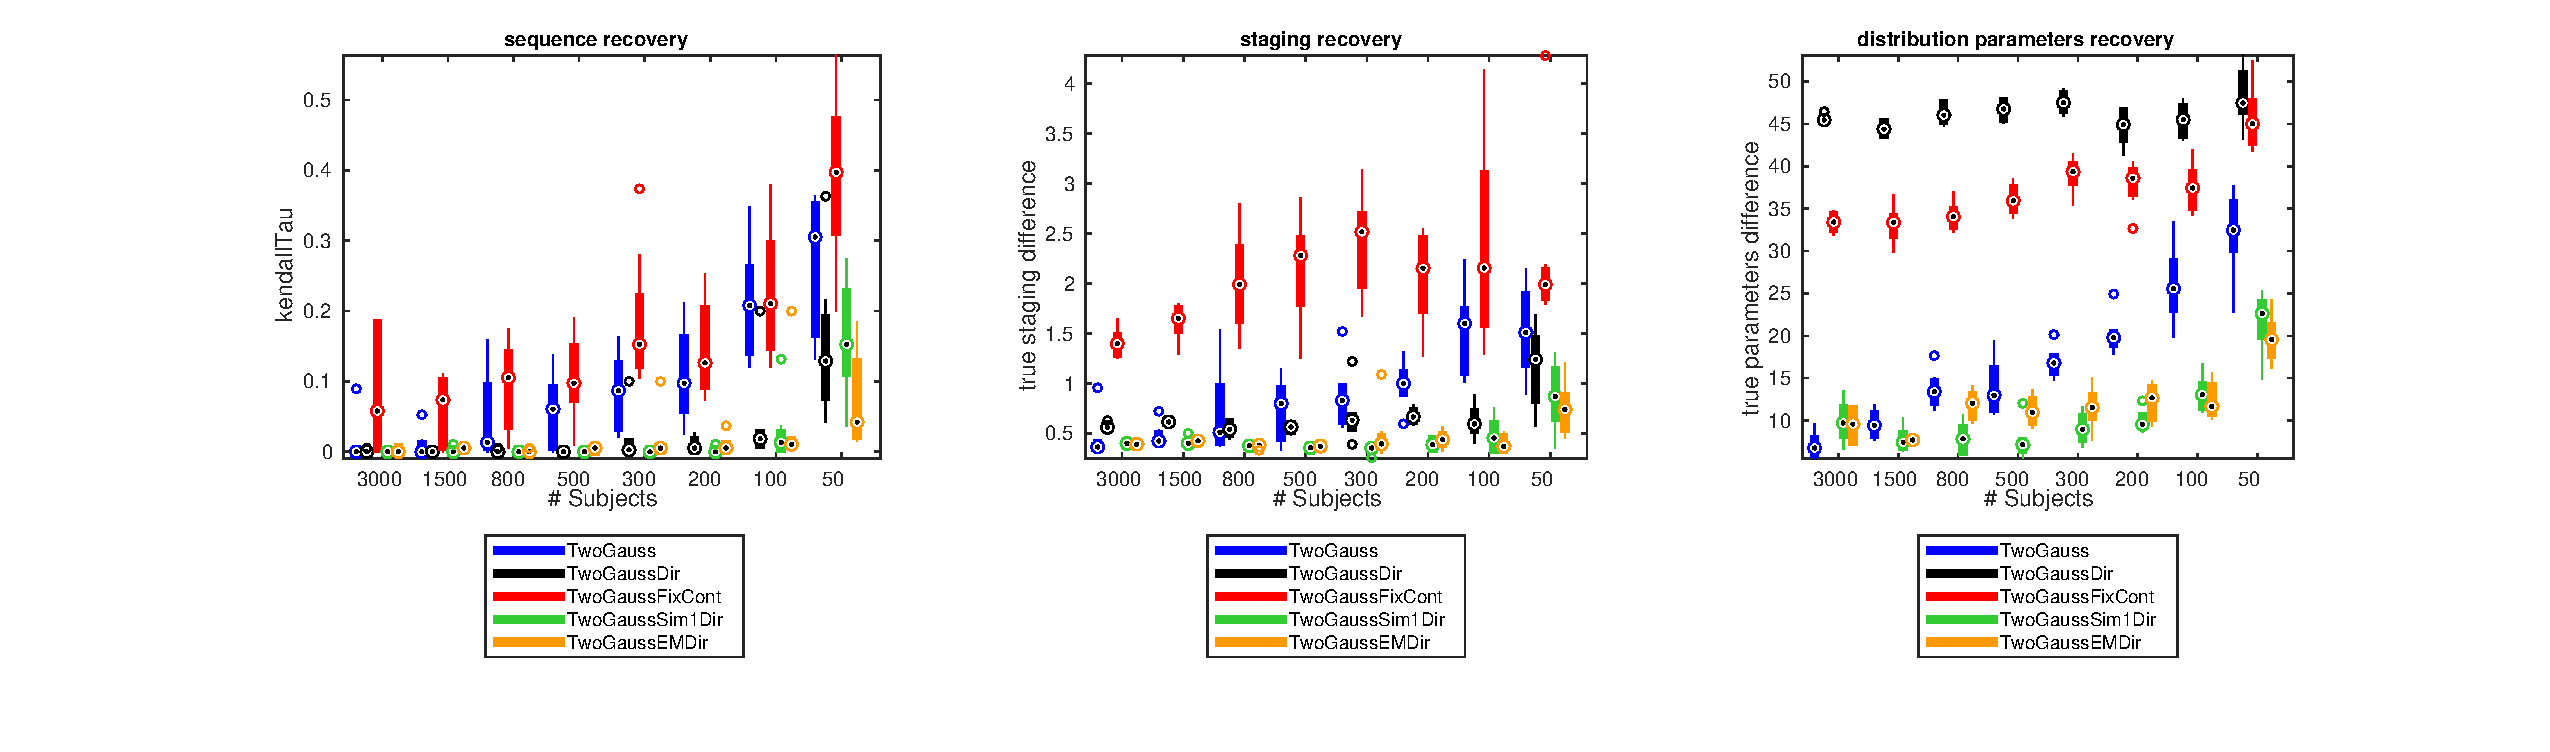
\includegraphics[scale=\simFigScale]{images/ebm/synthetic/metricsTwoGauss_incrSubj.eps}
\caption{Simulation results comparing different EBM model fitting methods. In blue we have the standard EBM method which first fits the distribution parameters and then the sequence, while in black and red we have the EBM Expectation-Maximisation method with two different starting points. Each of these three methods have been fit on eight synthetic datasets where we used a decreasing number of subjects, from 3000 down to 50. The left figure shows the Kendall-tau distance between the sequence recovered by the model and the true sequence. The middle figure shows the L1 norm of the difference between predicted subject stages and true stages. The right figure shows the L1 norm of the difference between the recovered distribution parameters and the true parameters.}
 \label{fig:incrSubjTG}
\end{figure}

\begin{table}[H]
\centering
\begin{tabular}{c | p{13cm}}
 TwoGauss & fit distribution parameters by optimising a mixture model, like Fontejin et al. \cite{fonteijn2012event}, Young et al. \cite{young2014data}\\
 TwoGaussDir & fitting each distribution directly on the control and patient data, optimise sequence independenly\\
 TwoGaussFixCont & fit the control distribution directly on control data, then fit patient distribution using mixture model optimisation.\\
 TwoGaussSim1 & simultaneous sampling of parameters and sequence, initialise the method from the solution found by TwoGauss\\
 TwoGaussSim1Dir & same as TwoGaussSim1, initialise the method from the solution found by TwoGaussDir\\
 
\end{tabular}
\caption{Legend description for Fig. \ref{fig:incrSubjTG}}
\end{table}

\begin{figure}[H]
%\centering
 \hspace{-2cm}
 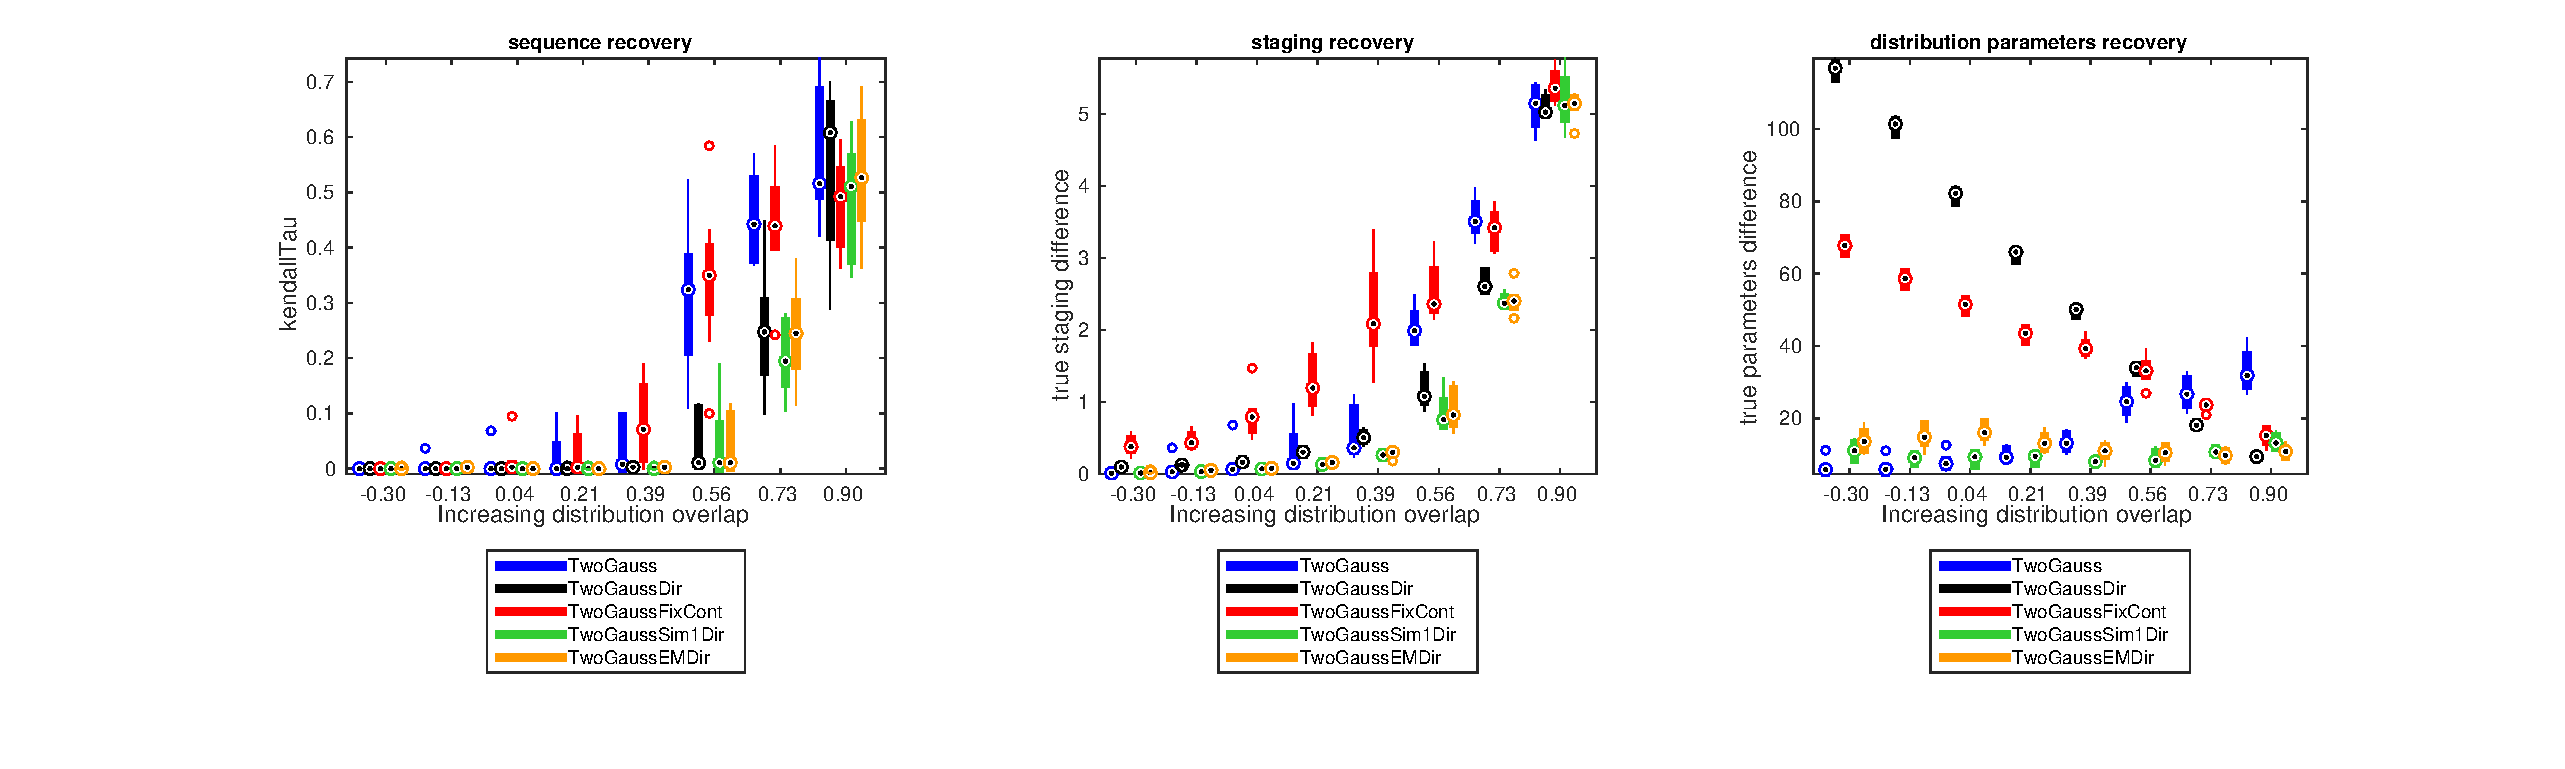
\includegraphics[scale=\simFigScale]{images/ebm/synthetic/metricsTwoGauss_incrDistOverlap.eps}
 \caption{Simulation results comparing different EBM model fitting methods. Same setup as in Fig. \ref{fig:incrSubjTG}, but this time we keep the number of subjects constant and instead increase the overlap of distributions $p(x|E)$ and $p(x| \neg E)$. The distribution overlap ranges from -0.3 (low overlap) to 0.9 (high overlap). } 
  \label{fig:incrDstTG}
\end{figure}

\begin{figure}[H]
%\centering
 \hspace{-2cm}
 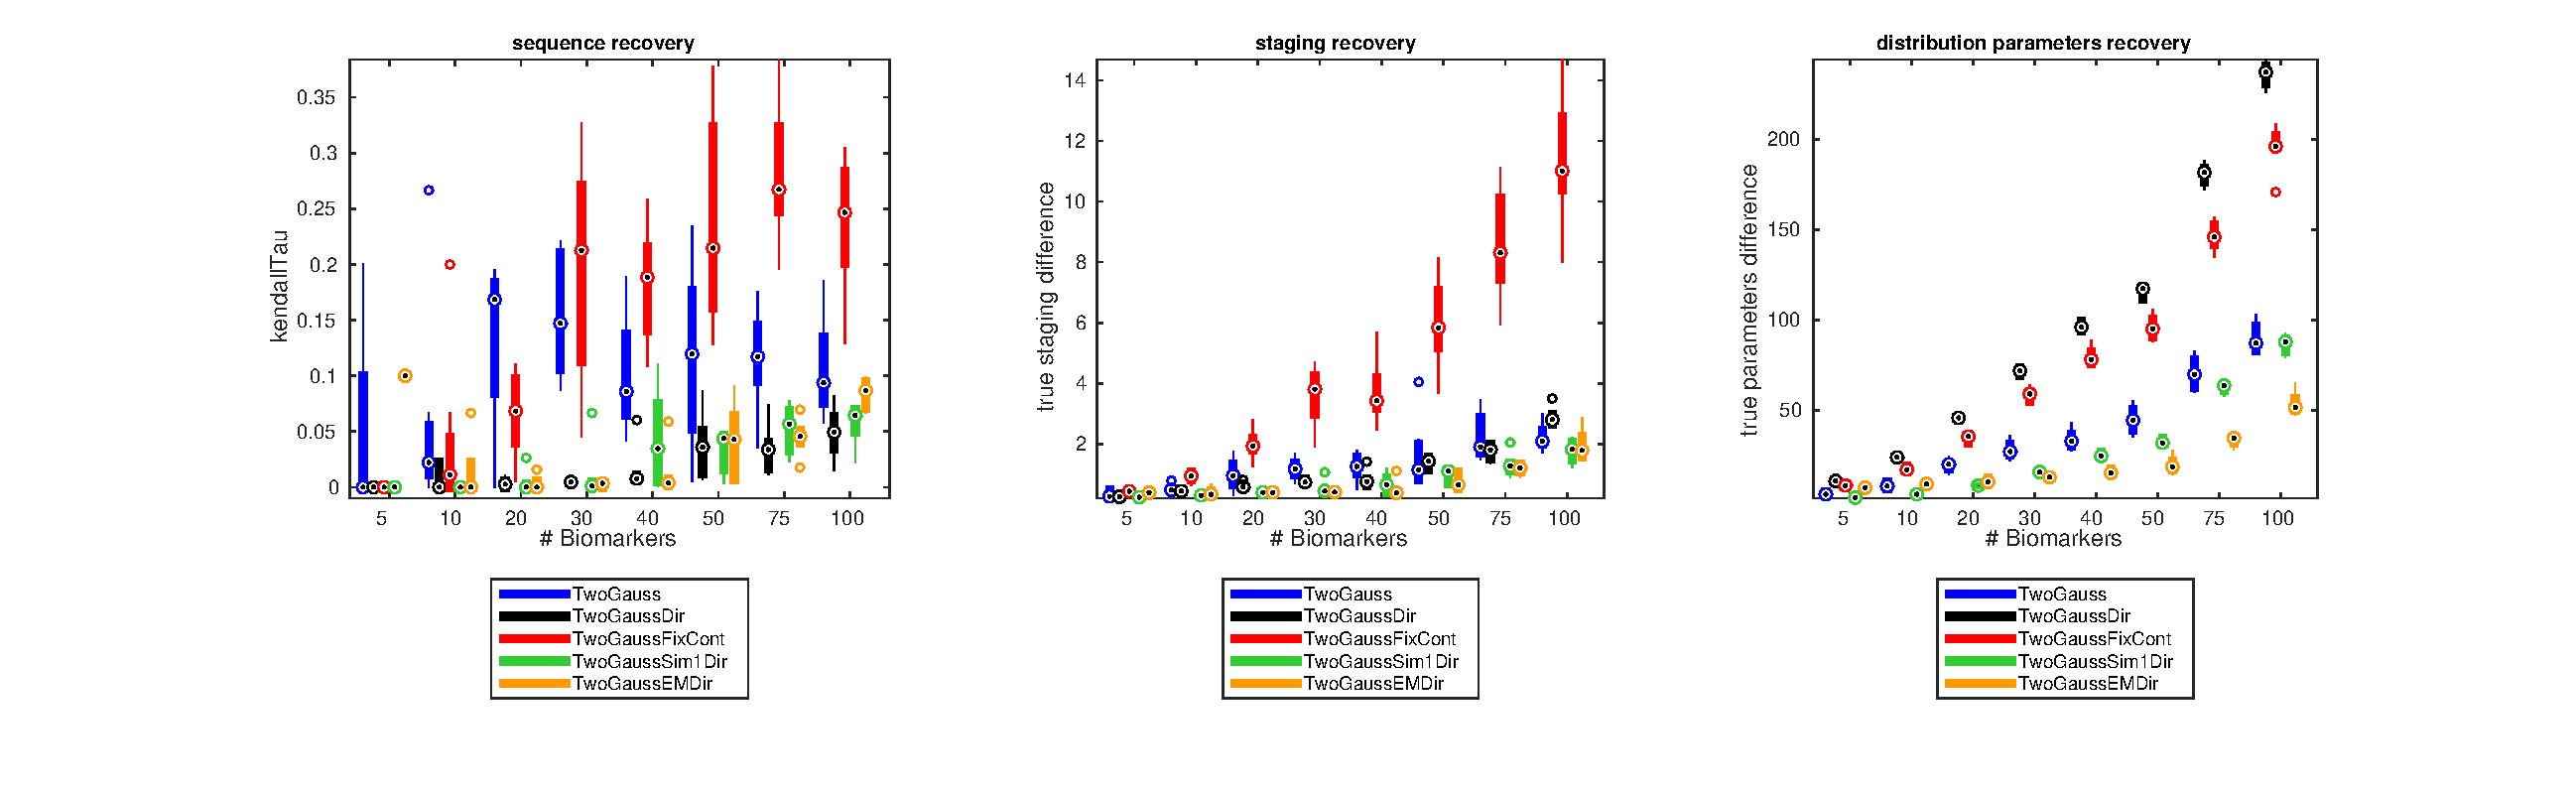
\includegraphics[scale=\simFigScale]{images/ebm/synthetic/metricsTwoGauss_incrBiomk.eps}
\caption{Simulation results comparing different EBM model fitting methods. Same setup as in Fig. \ref{fig:incrSubjTG}, but this time we keep the number of biomarkers used, from 0 to 100.}
  \label{fig:incBiomkTG}
\end{figure}

\begin{figure}[H]
%\centering
 \hspace{-2cm}
 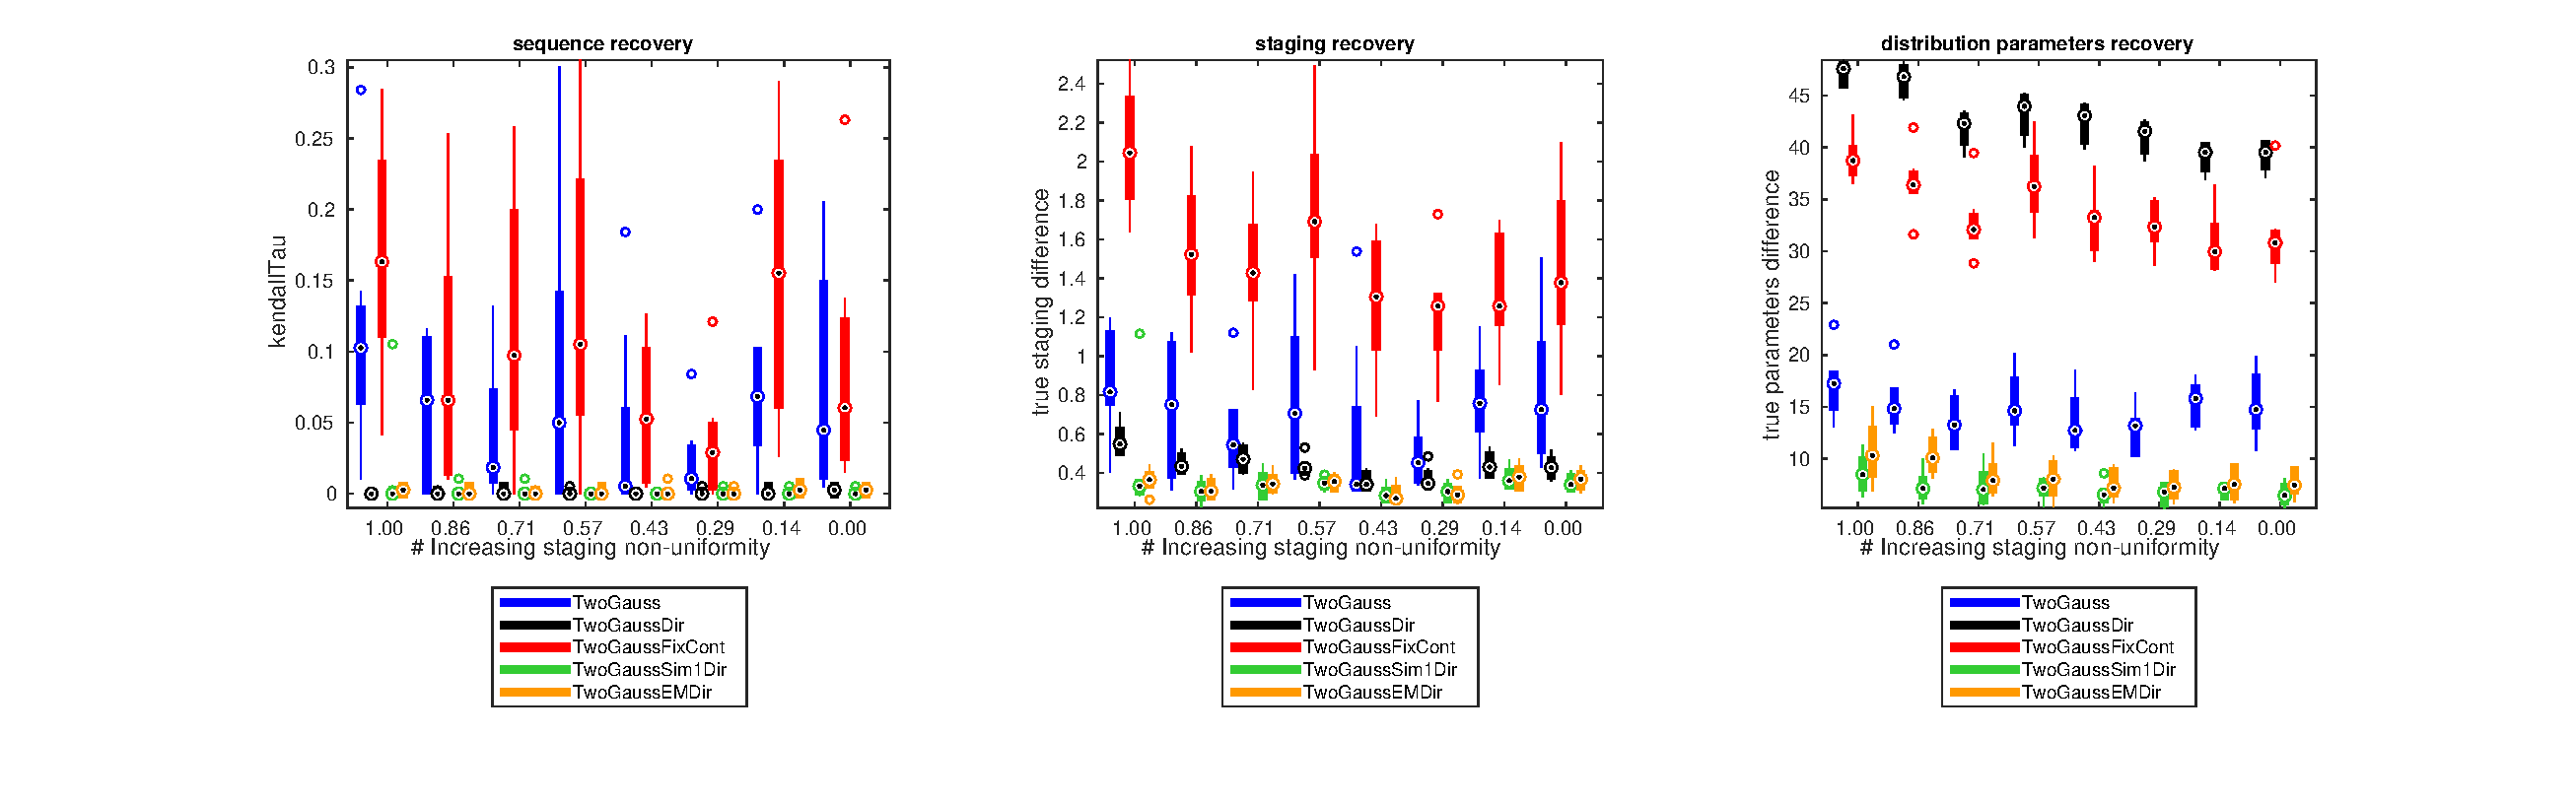
\includegraphics[scale=\simFigScale]{images/ebm/synthetic/metricsTwoGauss_incrStagingUnif.eps}
 \caption{Simulation results comparing different EBM model fitting methods. Same setup as in Fig. \ref{fig:incrSubjTG}, but this time we vary the uniformity of the subject stages, ranging from 1 (uniform probability across the disease timecourse) to 0 (subjects are placed more at beginning or end stages). The pdfs of the stage distributions for each experiment are shown in Fig. \ref{fig:StagingCurvesTG}. }
  \label{fig:incrStagTG}
\end{figure}

\begin{figure}[H]
 \centering
 \hspace{-2cm}
 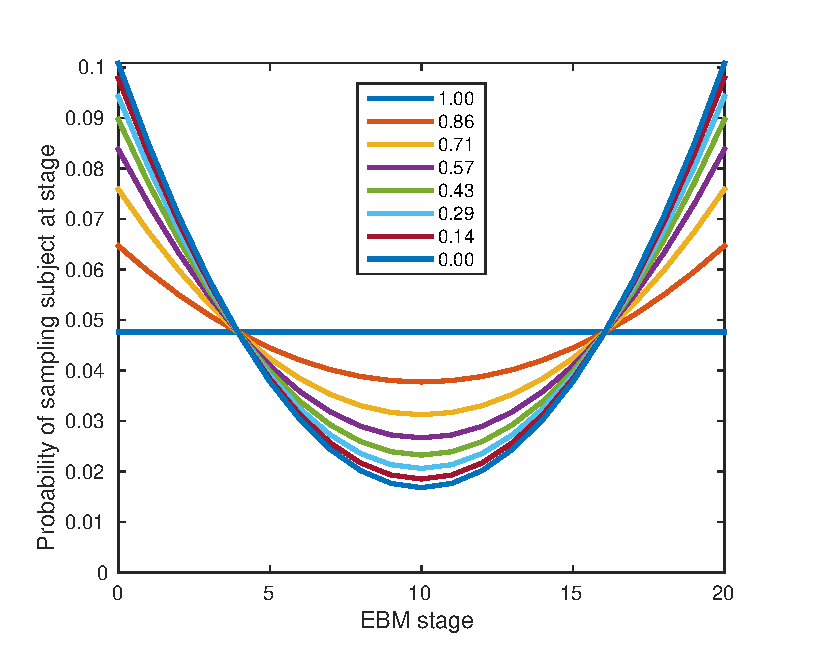
\includegraphics[scale=\simFigScale]{images/ebm/synthetic/stagingUnifCurves.eps}
 \caption{Pdf of the staging probability functions used to generate the synthetic datasets in Fig. \ref{fig:incrStagTG}. The shapes of the pdf distributions are quadratic curves for which we vary the second-order factor.}
 \label{fig:StagingCurvesTG}
\end{figure}

\begin{figure}[H]
%\centering
 \hspace{-2cm}
 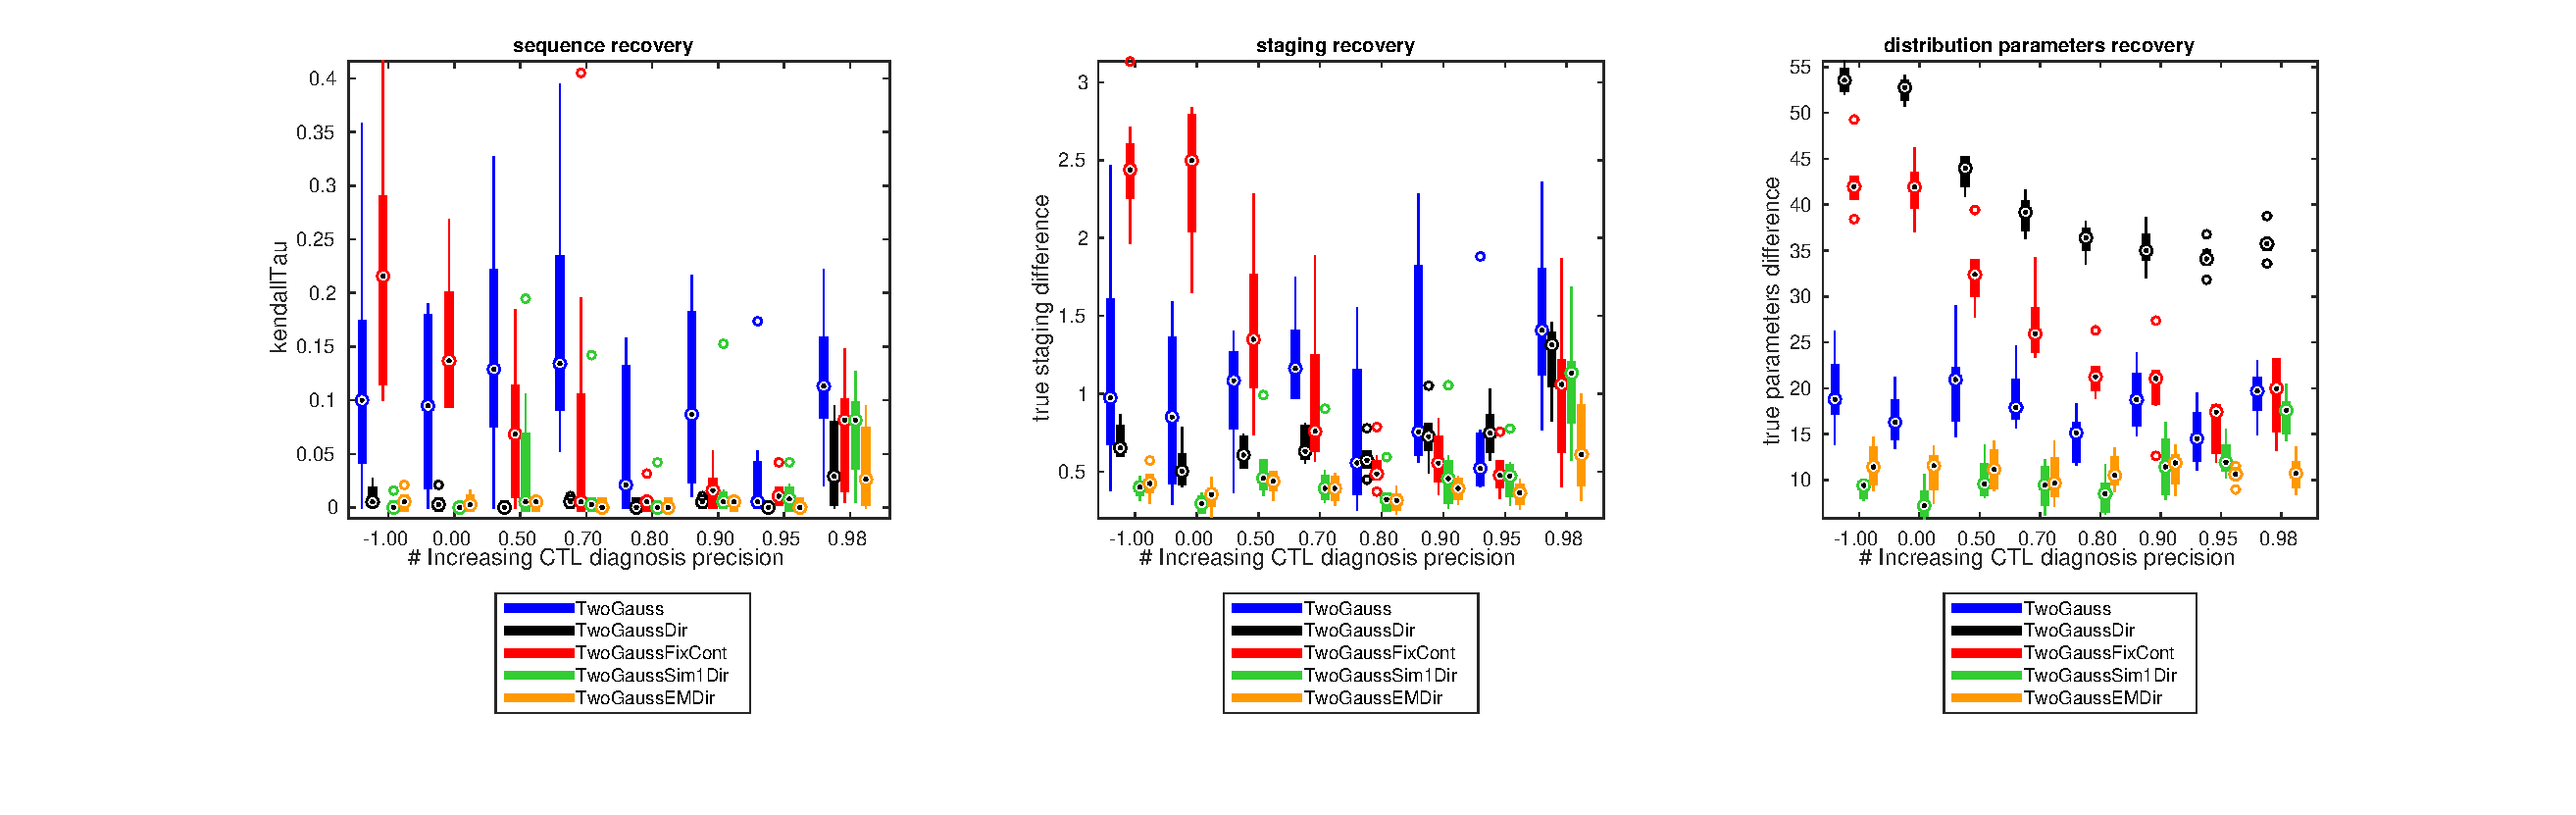
\includegraphics[scale=\simFigScale]{images/ebm/synthetic/metricsTwoGauss_incrCtlPrec.eps}
 \caption{Simulation results comparing different EBM model fitting methods. Same setup as in Fig. \ref{fig:incrSubjTG}, but this time we vary the precision of the control distribution, ranging from -1 (well-defined control population) to 1 (not so well defined control population). The pdfs of the stage distribution for control subjects in each experiment are shown in Fig. \ref{fig:ctlPrecCurvesTG}. }
  \label{fig:incrCtlPrecTG}
\end{figure}

\begin{figure}[H]
 \centering
 \hspace{-2cm}
 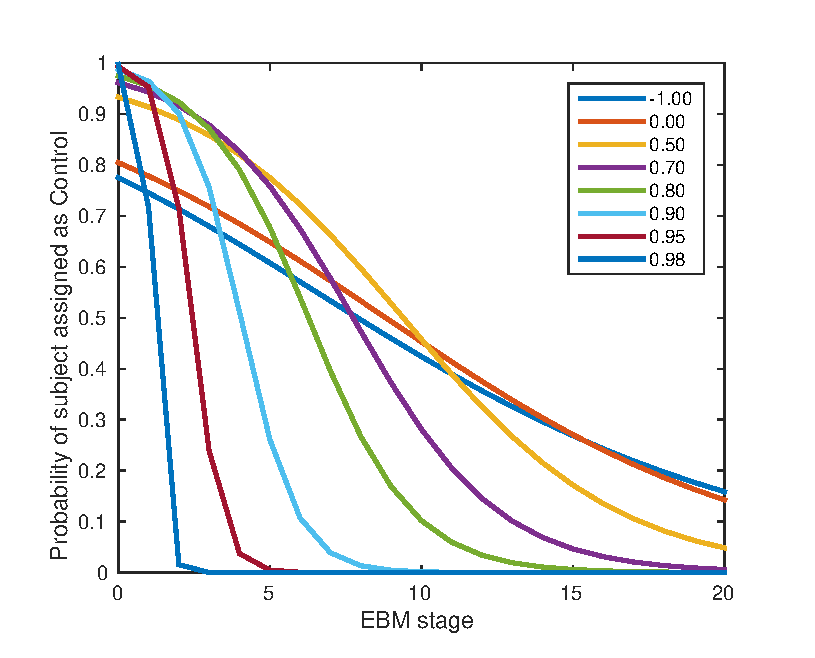
\includegraphics[scale=\simFigScale]{images/ebm/synthetic/ctlPrecCurves.eps}
 \caption{Probability density functions for the sampling distribution of the stages of controls. This ranges from -1 (well-defined control population) to 1 (not so well defined control population)}
 \label{fig:ctlPrecCurvesTG}
\end{figure}


\end{document}
